\documentclass[twoside]{article} 

\usepackage{macros}

\begin{document}

\twocolumn[

\aistatstitle{UCB with clustering and improved exploration}

\aistatsauthor{ }

\aistatsaddress{ } ]

\begin{abstract}

In this paper, we present a novel algorithm for the stochastic multi-armed bandit problem. Our proposed method, referred to as ClusUCB, partitions the arms into clusters and then follows the UCB-Improved strategy with aggressive exploration factors to eliminate sub-optimal arms as well as clusters. 
Through a theoretical analysis, we establish that ClusUCB achieves a better gap-dependent regret upper bound than UCB-Improved\cite{auer2010ucb} and MOSS\cite{audibert2009minimax} algorithms. Further, numerical experiments on test-cases with small gaps between optimal and sub-optimal mean rewards show that ClusUCB results in lower cumulative regret than several popular UCB variants as well as MOSS and Thompson sampling.
 %bandit algorithms such as UCB1\cite{auer2002finite}, UCB-Improved, MOSS, UCB-V\cite{audibert2009exploration}, Thompson Sampling\cite{agrawal2011analysis},Median Elimination\cite{even2006action}, KL-UCB\cite{garivier2011kl} and DMED\cite{honda2010asymptotically}.

%Old Abstract 27.8.2016

%In this paper, we present a novel algorithm which achieves a better upper bound on regret for the stochastic multi-armed bandit problem then some of the existing algorithms. Our proposed method clusters arms based on their average estimated payoff. This results in a more efficient elimination of arms within clusters as well as the deletion of weak clusters. We prove the regret upper bound  as 
%$\sum_{i\in B_{m}}\bigg (\max{\bigg\lbrace \bigg(\dfrac{32}{(\Delta_{i})^{3}}\bigg) ,\bigg(\dfrac{25\Delta_{i}}{(\Delta^{2})(0.16T\Delta^{2})^{2|B_{m}|^{2}\Delta/5}}\bigg)\bigg\rbrace} + \bigg(\Delta_{i}+\dfrac{32\log{(T\dfrac{\Delta_{i}^{4}}{16})}}{\Delta_{i}}\bigg)\bigg)$, $\Delta$ is the minimal gap between the means of the reward distributions of the optimal arm and a sub-optimal arm, $A$ is the set of arms, $T$ is the horizon and $\psi(m)$ is a parameter of the problem. This bound improves upon the existing algorithm of UCB-Revisited, MOSS, KL-UCB and UCB1 under certain cases. We corroborate our findings both theoretically and empirically and show that by sufficient tuning of parameter, we can achieve a lower regret than all the algorithms mentioned. In particular, in the test-cases where the arm set is dominated by small $\Delta$ and large $K$ we achieve a significantly lower cumulative regret than these algorithms.

%Old Abstract

%In this paper we achieve a lower regret bound by a novel method of using clustering of arms based on their average estimated payoff. By clustering of arms we divide the larger problem into smaller sub-problems and individually solve the sub-problems to arrive at a global solution. We prove that by this method we achieve a regret bound of the order of $O\bigg(K\log(KT\Delta^{2})\bigg)$ where $\Delta$ is the minimal gap between the means of the reward distributions of the optimal arm and a sub-optimal arm , $K$ is the number of arms and $T$ is the horizon. This improves upon UCB-Revisited having regret bound $O\bigg(K\dfrac{\log(T\Delta^{2})}{\Delta}\bigg)$ . This bound also improves upon UCB1 which has a regret of $O\bigg(\dfrac{K\log T}{\Delta}\bigg)$ and MOSS which has a minimax distribution free upper bound on the regret in the order of $O(\sqrt{TK})$ and a distribution dependent upper bound of $O\bigg(\dfrac{K\log(T\Delta^{2}/K)}{\Delta}\bigg)$. We corroborate our findings empirically and showed that by 
%sufficient tuning of some parameters we can achieve a lower regret than all the existing algorithms mentioned.
%\dots
%\keywords{Multi-Armed Bandit, UCB, Exploration-Exploitation, Clustering}
\end{abstract}

\section{Introduction}
\label{sec:intro}
In this paper, we consider the stochastic multi-armed bandit problem, a classical problem in sequential decision making. In this setting,  a learning algorithm is provided with a set arms with reward distributions unknown to the algorithm. The learning proceeds in an iterative fashion, where in each round, the algorithm chooses an arm and receives a stochastic reward that is drawn from a stationary distribution specific to the arm selected.  
Given the goal of maximizing the cumulative reward, the learning algorithm faces the exploration-exploitation dilemma, i.e., in each round should the algorithm select the arm which has the highest observed mean reward so far 
(\textit{exploitation}), or should the algorithm choose a new arm to gain more knowledge of the true mean reward of the arms and thereby avert a sub-optimal greedy decision (\textit{exploration}). 

Formally, let $r_i$, $i=1,\ldots,K$ denote the mean rewards of the $K$ arms and $r^* = \max_i r_i$ the optimal mean reward. The objective in the stochastic bandit problem is to minimize the cumulative regret, which is defined as follows:
\begin{align*}
R_{T}=r^{*}T - \sum_{i\in A} r_{i}N_{i},
\end{align*}
where $T$ is the number of rounds, $N_{i}=\sum_{m=1}^n I(I_m=i)$ is the number of times the algorithm chose arm $i$ up to round $T$.
The expected regret of an algorithm after $T$ rounds can be written as
%\newline
%\newline
\begin{align*}
\E[R_{T}]= \sum_{i=1}^K \E[N_i] \Delta_i,
\end{align*}
where $\Delta_{i}=r^{*}-r_{i}$ denotes the gap between the means of the optimal arm and of the $i$-th arm. 


%The problem, gets more difficult when the $\Delta_{i}$'s are smaller and arm set is larger. Also let $\Delta=min_{i\in A}\Delta_{i}$, that is it is the minimum possible gap over all arms in $A$.
                                                                                                                                          

%NEW RELATED WORK AND CONTRIBUTION

An early work involving a bandit setup is \cite{thompson1933likelihood}, where the author deals the problem of choosing between two treatments to administer on patients who come in sequentially. Following the seminal work of Robbins \cite{robbins1952some}, bandit algorithms have been extensively studied in a variety of applications. 
From a theoretical standpoint, an asymptotic lower bound for the regret was established in \cite{lai1985asymptotically}. In particular, it was shown there that for any consistent allocation strategy, we have
$$\liminf_{T \to \infty}\frac{\E[R_{T}]}{\log T}\geq\sum_{\{i:r_{i}<r^{*}\}}\dfrac{(r^{*}-r_{i})}{D(p_{i}||p^{*})},$$
where $D(p_{i}||p^{*})$ is the Kullback-Leibler divergence between the reward densities $p_{i}$ and $p^{*}$, corresponding to arms with mean $r_{i}$ and $r^{*}$, respectively.

	There have been several algorithm with strong regret guarantees. The foremost among them is UCB1 \cite{auer2002finite}, which has a regret upper bound of $O\bigg(\dfrac{K\log T}{\Delta}\bigg)$, where $\Delta = \min_{i:\Delta_i>0} \Delta_i$. This result is asymptotically order-optimal for the class of distributions considered. However, the worst case regret of UCB1  can be as bad as $\Omega \bigg(\sqrt{TK\log T}\bigg)$ - see \cite{audibert2009minimax}.  In the latter reference, the authors propose the MOSS algorithm and establish that the worst case regret of MOSS is $O\bigg(\sqrt{TK}\bigg)$ which improves upon UCB1 by a factor of order $\sqrt{\log T}$ and a gap-dependent regret of $\sum_{i:\Delta_{i}>0}\dfrac{K\log(2+T\Delta_{i}^{2}/K)}{\Delta_{i}}$. However, in certain regimes, the gap-dependent regret bound of MOSS can be worse than UCB1\todos{What regime is this? Can you give a reference here?}. The UCB-Improved algorithm, proposed in \cite{auer2010ucb}, is a round-based algorithm variant of UCB1 that 
has a gap-dependent regret bound of $O\bigg(\dfrac{K\log T\Delta^{2}}{\Delta}\bigg)$ and a worst case regret of $O\bigg(\sqrt{TK\log K}\bigg)$. An algorithm is \textit{round-based} if it pulls all the arms equal number of times in each round and then proceeds to eliminate one or more arms that it identifies to be sub-optimal. 
	
	%But this algorithm performs worse empirically as stated in \cite{lattimore2015optimally}. \textit{In this work we try to address one of the open questions as raised in \cite{bubeck2012regret} that is to find an algorithm with regret always better than MOSS and UCB-Improved.}
	%
	%In this context of Multi-Armed Stochastic Bandit, we will also like to mention some of the variance based algorithm such as UCB-Normal(\cite{auer2002finite}) , UCB-Tuned(\cite{auer2002finite}) and UCB-Variance(\cite{audibert2009exploration}) which shows that variance-aware algorithms tend to perform better than the algorithms that don't(UCB1, UCB-Improved, MOSS). It can be shown that  when the variance of some sub-optimal arm is lower, a variance-aware algorithm detects it quickly thereby reducing  regret. \textit{We test our algorithm against such variance-aware techniques and do an empirical analysis.} 
	%
	%A discussion on some recent algorithms employing divergence based techniques must also be done. Firstly, the algorithm proposed in \cite{honda2010asymptotically} the authors come up with the algorithm Deterministic Minimum Empirical Divergence also called DMED$+$(as referred by \cite{garivier2011kl}) which is first order optimal(they only give asymptotic guarantees). This algorithm keeps a track of arms whose empirical mean are close to the optimal arm and takes help of large deviation ideas to find the optimal arm. Secondly, the more recent algorithm called KL-UCB(\cite{garivier2011kl}) using KL-Divergence comes up with an upper bound on regret as $\sum_{i:\Delta_{i}>0}\bigg(\dfrac{\Delta_{i}(1+\alpha)\log T}{D(r_{i},r^{*})}+C_{1}\log\log T+\dfrac{C_{2}(\alpha)}{T^{\beta(\alpha)}}\bigg)$ which is strictly better than UCB1 as we know from Pinsker's inequality $D(r_{i},r^{*}) > 2\Delta_{i}^{2}$. KL-UCB beats UCB1, MOSS and UCB-Tuned in various scenarios. \textit{We empirically test against this algorithm 
% and show that in certain regimes our algorithm performs better than KL-UCB and DMED.}
	%
	%We also make a distinction between round-based algorithms like UCB-Improved, Successive Reject(\cite{audibert2010best}), Successive Elimination(\cite{even2006action}) and Median-Elimination(\cite{even2006action}) whereby the algorithm pulls all the arms equal number of times in each round/phase, then proceeds to eliminate some number of arms it identifies to be sub-optimal with high probability and this continues till you are left with one arm. \textit{Our algorithm is also a round based algorithm}. Finally, we must point out that our setup is strictly limited to stochastic scenario as opposed to adversarial setup as studied in the paper \cite{auer2002nonstochastic} where an adversary sets the reward for the arms for every timestep.
	
\paragraph{Our Work}
As mentioned in a recent work \cite{liu2016modification}, UCB-Improved has two shortcomings: 	
\begin{inparaenum}[\bfseries (i)]
\item a significant number of pulls are spend in early exploration, since UCB-Improved pulls all the arms $n_{m}=\bigg\lceil \dfrac{ 2\log(T\tilde{\Delta}^{2}_{m})}{\tilde{\Delta}^{2}_{m}} \bigg\rceil$ during the $m$-th round. The quantity $\tilde{\Delta}_{m}$ is initialized to $1$ and halved after every round.
\item In UCB-Improved, arms are eliminated conservatively, i.e, only after $\tilde{\Delta}_{m}<\dfrac{\Delta_{i}}{2}$, the sub-optimal arm $i$ is discarded. This is disadvantageous when $K$ is large and the gaps are identical ($r_{1}=r_{2}=..=r_{K-1}<r^{*}$) and small.
\end{inparaenum}
% 	To counter early exploration in \cite{liu2016modification} as well as in our algorithm we propose an exploration regulatory factor to control exploration. \textit{Our algorithm is also not an anytime algorithm}(neither is MOSS, UCB-Improved) and in this context we point out that knowledge of the horizon actually facilitates learning as it can exploit more information(as stated in \cite{lattimore2015optimally}). We also employ a couple of more strategies to bring down our regret as summarized below:-

We propose a variant of UCB algorithm (henceforth referred to as ClusUCB) that incorporates clustering and an improved exploration scheme. ClusUCB is a round-based algorithm that
starts with a partition of the arms into small clusters, each having uniform set of arms. 
The clustering is done at the start with a pre-specified the number of clusters. 
Each round of ClusUCB involves both (individual) arm elimination as well as cluster elimiation. While the conditions governing the arm and cluster eliminations are inspired by UCB-Improved, though the exploration factors governing these conditions are relatively more aggressive than that in UCB-Improved. 

From a theoretical analysis that involves carefully setting the exploration factors for arm and cluster elimination conditions, we observe that the gap-dependent regret of ClusUCB is better than that of UCB-Improved, while the worst-case regret is of the same order. While ClusUCB improves the regret bounds of UCB-Improved, it does not achieve the gap-independent bound of $O(\sqrt{KT})$ of MOSS. However, the gap-dependent bound of ClusUCB is better than MOSS.

On a setup with $r_{1}=r_{2}=..=r_{K-1}<r^{*}$ and $\Delta_{i}$'s are small and $K$ is large, we empirically demonstrate that ClusUCB outperforms UCB-Improved\cite{auer2010ucb}, MOSS\cite{audibert2009minimax} as well as other popular stochastic bandit algorithms such as DMED\cite{honda2010asymptotically}, UCB-V\cite{audibert2009exploration} and KL-UCB\cite{garivier2011kl}.

% 	Summarizing our contributions below:-
% \begin{enumerate}
% \item We propose a cluster based round-wise algorithm with two arm elimination conditions in each round.
% \item We achieved a lower regret upper bound(Theorem1,table in Appendix F) than UCB-Improved(\cite{auer2010ucb}), UCB1(\cite{auer2002finite}) and  MOSS (\cite{audibert2009minimax} which we verify both theoretically and empirically.
% \item Our algorithm also empirically compares well with DMED, UCB-Varinace and KL-UCB.
% \item In the critical case when $r_{1}=r_{2}=..=r_{K-1}<r^{*}$ and $\Delta_{i}$'s are small and $K$ is large which is encountered frequently in web-advertising domain (as stated in \cite{garivier2011kl}) this approach has a significant advantage over other methods.
% \item The only parameter that needs to be pre-specified to the algorithm is the number of clusters to be formed but unlike KL-UCB our algorithm parameter $p$ is not distribution-specific and also our algorithm does not involve calculation of a complex, time consuming function like the divergence function of KL-UCB.
% %though the authors specified in \cite{garivier2011kl} that for optimal result only one should use the divergence function specific to the type of distribution.
% %\item We also provide a short discussion on what other applications our algorithm can be employed successfully.
% \end{enumerate}
	
The rest of the paper is organized as follows: In Section \ref{sec:clusucb}, we present the ClusUCB algorithm. In Section \ref{sec:results}, we present the associated regret bounds and sketch the proofs in Section \ref{sec:proofsketch}. In Section \ref{sec:expts}, we present the numerical experiments and provide concluding remarks in Section \ref{sec:conclusions}. 


\section{Clustered UCB}
\label{sec:clusucb}
\paragraph{Notation.}
\label{sec:prelims}
We denote the set of arms by $A$, with the individual arms labeled $i, i=1,\ldots,K$.
We denote an arbitrary round of ClusUCB by $m$. We denote an arbitrary cluster by $s_{k}$, the subset of arms within the cluster $s_k$ by  $A_{s_{k}}$ and the set of clusters by $S$ with $|S|=p\leq K$. 
Here $p$ is a pre-specified limit for the number of clusters.
For simplicity, we assume that the optimal arm is unique and denote it by ${*}$, with $s^{*}$ denoting the corresponding cluster.
 %and the subset of arms in $s^{*}$ is denoted by $A_{s^{*}}$. 
The best arm in a cluster $s_{k}$ is denoted by $a_{max_{s_{k}}}$.  
We denote the sample mean of the rewards seen so far for arm $i$ by $\hat{r_i}$ and for the best arm within a cluster $s_k$ by $\hat{r}_{a_{\max_{s_{k}}}}$. 
%The exploration regulatory factor is denoted by $\psi$. The arm and cluster elimination parameters are denoted by $\rho_{a}$ and $\rho_{s}$ respectively. 
%$\Delta_{i}^{'}=r_{a_{\max_{s_{k}}}} - r_{i}$, such that $a_{i}\in s_{k}$.
% The variable $B_{m}$ denotes the arm set containing the arms that are not eliminated till round $m$.
%  The exploration regulatory factor is denoted by $\psi_{m}$. %\todos{\textit{``$\hat{r}_{min_{s_{i}}}\in s_{i}$ as the arm with minimum estimated payoff''}. $\hat{r}_{min_{s_{i}}}\in s_{i}$ is the minimum estimated payoff and not the arm corresponding to min est payoff. Similar writing pops up at several other places, for e.g., in the statements of the propositions. (Subho) Changed the line as saying the minimum/maximum estimated payoff}
%The parameter $\psi(m)$ is a monotonically decreasing function over the rounds, that is $\psi(m+1)\leq \psi(m)$. 
%Also, we define $w\geq 2$, a weight factor.
We assume that all arms' rewards are bounded in $[0,1]$.


%worst arm within a cluster $s_i$ by $\hat{r}_{min_{s_{k}}}\in s_{k}$

\subsubsection*{The algorithm}

Algorithm~\ref{alg:clusucb} presents the pseudocode of ClusUCB.

%%%%%%%%%%%%%%%% alg-custom-block %%%%%%%%%%%%
\algblock{ArmElim}{EndArmElim}
\algnewcommand\algorithmicArmElim{\textbf{\em Arm Elimination}}
 \algnewcommand\algorithmicendArmElim{}
\algrenewtext{ArmElim}[1]{\algorithmicArmElim\ #1}
\algrenewtext{EndArmElim}{\algorithmicendArmElim}

\algblock{ClusElim}{EndClusElim}
\algnewcommand\algorithmicClusElim{\textbf{\em Cluster Elimination}}
 \algnewcommand\algorithmicendClusElim{}
\algrenewtext{ClusElim}[1]{\algorithmicClusElim\ #1}
\algrenewtext{EndClusElim}{\algorithmicendClusElim}

\algtext*{EndArmElim}
\algtext*{EndClusElim}

\begin{algorithm}[t]
\caption{ClusUCB}
\label{alg:clusucb}
\begin{algorithmic}
\State {\bf Input:} A partition of $A$ into clusters from Algorithm \ref{alg:rua}, exploration parameters $\rho_a$, $\rho_s$, time horizon $T$.
\State {\bf Initialization:} Set $B_{0}:=A$, $\psi=\log T$, $\epsilon_{0}:=1$ and $w_{0}:=1$.
%\State For rounds $m=1,2,.. \lceil\frac{1}{2}\log T\rceil$
\For{$m=0,1,..\big \lfloor \dfrac{1}{2}\log_{2} \dfrac{T}{e}\big\rfloor$}	
\State Pull each arm in $s_{k}$ $n_{m}=\bigg\lceil\dfrac{2\log{(\psi T\epsilon_{m}^{2})}}{\epsilon_{m}}\bigg\rceil$ number of times, $\forall s_{k}\in S$ 
%\State \hspace*{2em} Calculate $w_{s_{i}}=\bigg\lceil\dfrac{1}{\ell\hat{\Delta}_{s_{i}}}\bigg\rceil$,if $\hat{\Delta}_{s_{i}}\neq 0, \forall s_{i}\in S$
%\newline\hspace*{8em}$=1$, otherwise, and $\hat{\Delta}_{s_{i}}=\max_{i\in s_{i}}{\lbrace\hat{r}_{i}\rbrace}-\min_{j\in s_{i}}{\lbrace\hat{r}_{j}\rbrace}, i\neq j$
\ArmElim
\State For each cluster $s_k \in S$, delete arm $a_{i}\in s_{k}$ if
$$\hat{r}_{i} + \sqrt{\dfrac{\rho_{a}\log{(\psi T\epsilon_{m}^{2})}}{2 n_{m}}}  < \max_{a_{j}\in s_{k}}\bigg\lbrace\hat{r}_{j} -\sqrt{\dfrac{\rho_{a}\log{(T\epsilon_{m}^{2})}}{2 n_{m}}} \bigg\rbrace.$$
% where $\rho_{a}=\dfrac{1}{w_{m}}$ and remove all such arms from $B_{m}$.
\EndArmElim
\ClusElim
\State Delete cluster $s_{k}\in S$ if 
\begin{align*}
 \max_{a_{i}\in s_{k}}\bigg\lbrace\hat{r}_{i} + \sqrt{\dfrac{\rho_{s}\log{(\psi T\epsilon_{m}^{2})}}{2 n_{m}}}\bigg\rbrace  \\
 < \max_{a_{j}\in B_{m}} \bigg\lbrace\hat{r}_{j} - \sqrt{\dfrac{\rho_{s} \log{(T\epsilon_{m}^{2})}}{2 n_{m}}}\bigg\rbrace.
\end{align*}
%  and remove all such arms in the cluster $s_{k}$ from $B_{m}$ to obtain $B_{m+1}$.
\EndClusElim
\State Set $\epsilon_{m+1}:=\dfrac{\epsilon_{m}}{2},w_{m+1}:=2w_{m}$
%\State \hspace*{2em} $\ell_{m+1}:=\min\lbrace 2\ell_{m}, K\rbrace$
%\State \hspace*{2em} $w_{m+1}:=2w_{m}$
\State Stop if $|B_{m}|=1$ and pull $\max_{a_{i}\in B_{m}}\hat{r}_{i}$ till $T$ is reached.
\EndFor
\end{algorithmic}
\end{algorithm}

ClusUCB begins with a initial clustering of arms that is performed by random uniform allocation - see Algorithm \ref{alg:rua}. The set of clusters $S$ thus obtained satisfies $|S|=p$, with individual clusters having a size that is bounded above by $\ell=\bigg\lceil \dfrac{K}{p} \bigg\rceil$.
%For creating these clusters we rely on the parameter $\epsilon_{m}$, which is initialized at $1$ and halved after every round. 
%$\hat{\Delta}_{m}$(in which all $\hat{r}_{i}$ lies) divided by $\ell$. 
%If the range before any round is found to be $0$ then we conduct a small exploration with the alternate definition of $\epsilon_{m}=\dfrac{1}{D_{m}}$. 
%Thus, we see that as the rounds progresses, $\epsilon_{m}$ gets smaller and smaller resulting in tighter and tighter clusters with high purity level. Single link clustering tends to create large clusters with many elements in a single cluster. To avoid this behavior, mainly because we are conducting exploration inside a cluster based on its size, we bound the maximum cluster size possible in any round by $\ell=\min\lbrace 2^{m}, K \rbrace$. Hence as $\epsilon_{m}$ tends to $\Delta$ the upper limit on the cluster size gets fixed. 

Each round of ClusUCB involves both individual arm as well as cluster elimination conditions that are inspired by UCB-Improved. Notice that, unlike UCB-Improved, there is no longer a single point of reference based on which we are eliminating arms. Instead now we have as many reference points to eliminate arms as number of clusters formed. 
Further, the exploration factors $\rho_{a}\in (0,1]$ and $\rho_{s}\in (0,1]$ governing the arm and cluster elimination conditions, respectively, are relatively more aggressive than that in UCB-Improved. The number $n_m$ of times each arm is pulled per round in ClusUCB is lower than that of UCB-Improved, which used $n_{m}=\bigg\lceil \dfrac{2log(T\epsilon_{m}^{2})}{\epsilon_{m}^{2}} \bigg\rceil$ and Median-Elimination, which used $n_m=\dfrac{4}{\epsilon^{2}}\log\big(\dfrac{3}{\delta}\big)$, where $\epsilon,\delta$ are confidence parameters.

We can be this aggressive because we have divided the larger problem into smaller sub-problems, doing local exploration and eliminating sub-optimal arms within each clusters with high probability. In particular, when $K$ is large and the gaps $\Delta_i$ are small, it is efficient to remove sub-optimal arms quickly rather getting tied down in hopeless exploration. 
The theoretical analysis confirms this intuition, as choosing $\rho_a=\rho_s = \max\lbrace \frac{1}{2},\frac{1}{2^m}\rbrace$ and $\psi_m=K^2T$, ClusUCB is able to achive a better gap-dependent regret upper bound as compared to UCB-Improved and MOSS. 
%Also our total regret depends on how many arms has survived till $m$-th round and so we don't need to keep track on the number of clusters formed.

%Through cluster elimination condition we ensure that the stopping condition is reached faster. This is a much aggressive elimination condition and in the proofs we give a further analysis on why this works. The parameter $\rho\in (0,1]$ in the confidence interval actually makes the cluster elimination a faster elimination condition than the elimination condition in UCB-Improved.
	
%This is a parameter which we use to tune our exploration and we define its structure later in the proofs. There is also the weight($w_{s_{i}}$) parameter which   is calculated online and helps in eliminating arms with a higher probability which we employ to reduce the cumulative regret and this parameter is decide online specific to the cluster $s_{i}\in S$.

\begin{algorithm}[t]
\caption{Clustering by random uniform allocation}
\label{alg:rua}
\begin{algorithmic}
\State Set $\ell=\bigg\lceil \dfrac{K}{p} \bigg\rceil$
\State Permute arms in $A$ randomly to create $A_{random}$.
\State Create clusters $s_{i}=\lbrace a_{i}\rbrace, \forall i\in A_{random}$
\For{ $i=1$ to $K$}
\For{$j=i+1$ to $K$}
\State Merge $s_{i},s_{j}$ into $s_{i}$ if $\exists a_{i}\in s_{i} $ and $\exists a_{j}\in s_{j},$ such that $|s_{i}|+|s_{j}|\leq \ell$
\EndFor
\EndFor
\State Rename all partitions that have been formed as $s_{1}$ to $s_{p}$, where $|S|=p$ after merging
\end{algorithmic}
\end{algorithm}





%\newpage
\section{Main results}
\label{sec:results}
	
	Here, we state the main theorem of the paper which shows the regret upper bound of ClusUCB.
	
\begin{theorem}
Considering both the arm elimination and cluster elimination condition, the total regret till $T$ is upper bounded by $R_{T}\leq \sum_{i\in A:\Delta\geq b} \bigg\lbrace 3\Delta_{i}+ \bigg(\dfrac{44}{\Delta_{i}^{3}}\bigg) + \bigg(\dfrac{2^{1+4\rho}\rho^{2\rho}T^{1-\rho}}{\Delta_{i}^{4\rho-1}}\bigg) + \bigg(\dfrac{32\log{(T\dfrac{\Delta_{i}^{4}}{16})}}{\Delta_{i}}\bigg) + \bigg(\dfrac{512\rho\log{(T\dfrac{\Delta_{i}^{4}}{16\rho^{2}})}}{\Delta_{i}}\bigg)\bigg\rbrace + \sum_{i\in A:0\leq\Delta_{i}\leq b}\bigg\lbrace \bigg(\dfrac{12}{b^{3}} \bigg) + \bigg(\dfrac{T^{1-\rho}2^{2\rho+\frac{3}{2}}}{\Delta_{i}^{3}} \bigg)+\bigg(\dfrac{T^{1-\rho}2^{2\rho+\frac{3}{2}}}{b^{4\rho -1}} \bigg) \bigg\rbrace + max_{i:\Delta\leq b}\Delta_{i}T $, where $\rho\in (0,1]$ and $T$ is the horizon.
\end{theorem}

\begin{proof}
	See Appendix.
\end{proof}

\begin{remark}
	Thus, we see the most significant term in the regret is $\dfrac{512\rho\log{(T\dfrac{\Delta_{i}^{4}}{12})}}{\Delta_{i}}$, which is significantly lower than UCB1, UCB2, EXP3, UCB($\delta$), MOSS, UCB-Revisited and Median Elimination under certain cases when the $\Delta \rightarrow 0$ and $K$ is large. Also ClusUCB is more efficient than UCB1, MOSS, EXP3, UCB($\delta$), KL-UCB as $K$ scales up because being a round-based algorithm, it is removing sub-optimal arms in each round as opposed to the former algorithms which are calculating the confidence bounds over all arms in each timestep and then choosing the max of them. %Also evident from the proof is that if the horizon $T$ is small or very large we can tune the parameter $\psi(m)$ carefully to have a lesser regret. For readers convenience a table is given in Appendix G on the various regret bounds of several algorithms. 
\end{remark}	


%\todos{(Subho)To follow the same way as UCB-Revisited proof, did away with the event $\xi_{1},\xi_{2},\xi_{3}$}

%In this section we will prove the bounds based on the events $\xi_{1}$,$\xi_{2}$ and $\xi_{3}$. In $\xi_{1}$, we will assume two important assumptions $i)\hat{r}^{*}<\hat{r}_{i},\forall i\in s_{i}$ and $ii)\exists a_{i}\in s_{i}$ such that $\sqrt{\dfrac{\epsilon_{m}}{w_{s_{i}}}}<\dfrac{\Delta_{i}}{5}$. For $\xi_{2}$, we will assume that $a^{*}\in s^{*}$ and $|s^{*}|=1$, $a_{i}\in s_{i} \forall a_{i}\setminus a^{*}\in B_{m}$ and $\exists a_{max_{s_{i}}}$ such that $\sqrt{\epsilon_{m}}<\dfrac{2\Delta_{s}}{5}$, where $\Delta_{s}=r^{*}-r_{max_{s_{i}}}$ and $\hat{r}_{max_{s_{i}}}>\hat{r}_{i}, \forall i\in s_{i}$. $\xi_{3}$ be the event when the optimal arm $a^{*}$ gets eliminated by a sub-optimal arm. At the start of any round $m$, we fix $\epsilon_{m}$.

\begin{remark}
A sketch of the proof is given here. In the first step, we try to calculate the number of pulls $n_{m}$ required to make the optimal arm  safe with a high probability so that it goes up atleast $\dfrac{\hat{\Delta}_{s_{i}}}{2}$ where $\hat{\Delta}_{s_{i}}=max_{i\in s_{i}}\hat{r}_{i}-min_{j\in s_{i}}\hat{r}_{j},i\neq j$. This is shown in Proposition 1. Second step, we try to bound the probability of arm elimination of any sub-optimal arm without cluster elimination. This is shown in Proposition 2. Third step, we try to bound the probability of cluster elimination(without any arm elimination) with all arms within it and the favourable event leading to it. This is shown in Proposition 3. Finally, in the proof of Theorem 1 we combine all these to get the regret bound.  
\end{remark}
	
\begin{proposition}
The probability that the optimal arm $a^{*}\in s_{i}$ will lie above $\hat{r}_{min_{s_{i}}}+ \dfrac{\hat{\Delta}_{s_{i}}}{2}$ after $\bigg\lceil\dfrac{2\log (\psi(m)T\epsilon_{m}^{2})}{\epsilon_{m}}\bigg\rceil$ pulls in the $m$-th round is given by $\bigg\lbrace 1- \dfrac{1}{(\psi(m)T\epsilon_{m}^{2})^{\ell_{m}^{2}\epsilon_{m}}} \bigg\rbrace$ where $\hat{r}_{min_{s_{i}}}$ is the minimum payoff in $s_{i}$, $\hat{\Delta}_{s_{i}}=max_{i\in s_{i}}\hat{r}_{i}-min_{j\in s_{i}}\hat{r}_{j}, i\neq j$, $\epsilon_{m}$ is halved after every round and $T$ is the horizon. 
\end{proposition}

%$\epsilon_{m}=\max{\bigg\lbrace\dfrac{\hat{\Delta}_{m}}{\ell_{m}} \dfrac{2}{\sqrt{\psi{(m)T}}}\bigg\rbrace}$

	The proof of Proposition 1 is given in \textbf{Appendix A}.(Supplementary material)

%\begin{remark}
%	Thus, we see that as the agent falls through rounds, with increasing values of $\ell_{m}$ the probability of optimal arm $a^{*}$ lying above $\dfrac{\hat{\Delta}_{s_{i}}}{2}$ increases as $\ell_{m}^{2}\epsilon_{m}\geq 4$ (as, $\epsilon_{m}$ is halved after every round and $\ell_{m}$ is doubled) increases with increasing $\ell_{m}$. But, $\ell_{m}$ is bounded by $D_{m}$ and say after the $m_{D}$ round the probability of optimal arm staying above the specified range gets bounded by $\bigg\lbrace 1- \dfrac{1}{(\psi(m)T\epsilon_{m}^{2})^{D_{m}^{2}\epsilon_{m}}} \bigg\rbrace$. But we know from the definition of $D_{m}$ that $ D_{m}=\bigg\lceil(\dfrac{1}{\epsilon_{m}})^{1/2}\bigg\rceil$ or $D^{2}\epsilon_{m}\approx 1$. Hence, the probability that   $a^{*}$ after $n_{m}$ pulls in round $m_{D}$ going above $\dfrac{\hat{\Delta}_{s_{i}}}{2}$ is $\bigg\lbrace 1- \dfrac{1}{(\psi(m)T\epsilon_{m}^{2}) }\bigg\rbrace$.

%	We must also point out that $\epsilon_{m}$ can become arbitrarily small, so the value $\log{(\psi{(m)}T\epsilon_{m}^{2})}$ can become negative. To guard against that scenario we have setup a tolerance level such as $\epsilon_{m}>\dfrac{2}{\sqrt{\psi{(m)}T}}$ and below this value $\epsilon_{m}$ should not be allowed to fall. 
%	We also see that $\ell_{m}$ is doubled after every round, independent of the rise in $D_{m}$ and as $\epsilon_{m}\rightarrow \Delta $, $\ell_{m}$ gets upper bounded by $D_{m}$ and will rise no more and hence $D_{m}$ also gets fixed as $D_{m}^{2}\epsilon_{m}\approx 1$ for any round $m$. We make the $D_{m}$ increase with the rounds as it controls our rate of exploration and in the later rounds we need more exploration as arms close to the optimal arm will survive till the later rounds and the algorithm needs to discriminate amongst them.  Also, if $\epsilon_{m}$ is very large, then $D_{m}$ becomes very small and consequently there is very small exploration. Hence, $D_{m}$ is the maximum of $\lbrace \dfrac{1}{\sqrt{\epsilon_{m}}}, K \rbrace$, which ensures the algorithm does sufficient exploration. 
%\end{remark}


%\todos{(Subho) Merged proposition 2 and 3 into one to follow the UCB-Revisited case (a)}

\begin{proposition}
Considering only the arm elimination condition, the total regret till $T$ is upper bounded by $R_{T}\leq \sum_{i\in A:\Delta_{i}\geq b}\bigg \lbrace \bigg(\dfrac{44}{(\Delta_{i})^{3}}\bigg) + \bigg(\Delta_{i}+\dfrac{32\log{(T\dfrac{\Delta_{i}^{4}}{16})}}{\Delta_{i}}\bigg)\bigg\rbrace + \sum_{i\in A:0\leq\Delta_{i}\leq b}\dfrac{12}{b^{3}} + max_{i:\Delta\leq b}\Delta_{i}T$, where $T$ is the horizon.
\end{proposition}

	The proof of Proposition 2 is given in \textbf{Appendix B}.(Supplementary material).

\begin{remark}
	
	Thus, we see that the confidence interval term $c_{m}=\sqrt{\dfrac{\log (T\epsilon_{m}^{2})}{2 n_{m}}}$ makes the algorithm eliminate an arm $a_{i}$ as soon as $\sqrt{\epsilon_{m}}<\dfrac{\Delta_{i}}{2}$. The above result is in contrast with UCB-Revisited which only deletes an arm if $\tilde{\Delta}_{m}<\dfrac{\Delta_{i}}{2}$, where $\tilde{\Delta}_{m}$ is initialized at $1$ and is halved after every round. We also see from our result that a much less stricter elimination condition is adopted inside a cluster. We are eliminating inside a cluster because we are exploring locally and we are guaranteed with  $\bigg\lbrace 1- \dfrac{2}{(T\epsilon_{m}^{2})^{\ell_{m}^{2}\epsilon_{m}}} \bigg\rbrace$ probability that in the $m$-th round optimal arm $a^{*}$ will atleast lie above $\hat{r}_{min_{s_{i}}}+ \hat{\Delta}_{s_{i}}$. 
%Also, the weight $w_{s_{i}}$ as shown in the proofs actually help us in faster elimination of arms by the condition $ii$ in $\xi_{1}$ explained at the start of the proof. The higher the weight faster is arm elimination but it also increases error probability which might actually lead to a higher cumulative regret. The weight $w_{s_{i}}$ depends on the cluster size and the larger the cluster size, the higher will be the weight increasing the probability of arm elimination as we want smaller and smaller number of elements in clusters so that we can discriminate effectively amongst the clusters.
%\end{remark}
%
%
%\begin{proposition}
%With a probability of $\bigg\lbrace 1-\bigg(\dfrac{2}{\psi(m)T\epsilon_{m}^{2})}\bigg)\bigg\rbrace$ a sub-optimal arm can be deleted within a cluster $s_{i}$ in round $m$ by the arm elimination condition, where $\epsilon_{m}=\max{\bigg\lbrace\dfrac{\hat{\Delta}_{s,m}}{\ell_{m}}, \dfrac{1}{\sqrt{\psi{(m)T}}}\bigg\rbrace}$, if $\hat{\Delta}_{s,m}\neq 0$ and $T$ is the horizon.
%\end{proposition}
%
%	The proof of Proposition 3 is given in \textbf{Appendix C}.(Supplementary material)	
%
%\begin{remark}
%	Thus, we see that the probability of a sub-optimal arm $a_{i}$ is eliminated in $\xi_{1}$ is  $\bigg(1-\dfrac{2}{\psi(m)T\epsilon_{m}^{2})}\bigg)$ which increases as the algorithm falls through the round as $\epsilon_{m}$ keeps on decreasing.
%	
%	Due to the initial uncertainty we can sufficiently tune $\psi(m)$ to increase our pulls in the initial rounds in a bounded fashion. But this function can be set arbitrarily high resulting in a skewed regret upper bound and so we need to define a structure and bound this function as well. We define $\psi(m)=\dfrac{c}{m}$ where $c>0, m\geq 1$ as defined previously. Notice also that $\psi(m)$ is a monotonically decreasing function and for any round $m$, $|\psi(m+1)|\leq |\psi(m)|$. 
%%In experiment 2 and 3 where $\psi(m)=K^{5/m}$ is defined since the variance is very high in those cases. 
%%Since $|\psi(m)|\geq 0,\forall m$, this also leads to increase in the probability of arm deletion as compared to UCB-Revisited.
%When the time horizon $T$ is very large or very small, as the pulls $n_{m}$ depends on $T$, we can tune $\psi(m)$ by changing $c$ so that the exploration remains balanced. Since we are exploring locally and the pulls are increasing after every round so we decrease $\psi(m)$ in the later rounds which not only tapers down the growth of $n_{m}$ but also decreases arm elimination probability, as in the later rounds, only arms closer to the optimal arm survive and we need careful elimination.
\end{remark}
	
	
	

\begin{proposition}
Considering only the cluster elimination condition, the total regret till $T$ is upper bounded by $R_{T}\leq \sum_{i\in A:\Delta_{i}\geq b}\bigg(\dfrac{2^{1+4\rho}\rho^{2\rho}T^{1-\rho}}{\Delta_{i}^{4\rho-1}}\bigg) + \bigg(\Delta_{i}+\dfrac{512\rho\log{(T\dfrac{\Delta_{i}^{4}}{16\rho^{2}})}}{\Delta_{i}}\bigg)  +  \bigg(\dfrac{T^{1-\rho}2^{2\rho+\frac{3}{2}}}{\Delta_{i}^{4\rho -1}} \bigg) \bigg \rbrace+\sum_{i\in A:0\leq\Delta_{i}\leq b}\bigg(\dfrac{T^{1-\rho}2^{2\rho+\frac{3}{2}}}{b^{4\rho -1}} \bigg) + max_{i:\Delta\leq b}\Delta_{i}T$, where $\rho\in (0,1)$ and $T$ is the horizon.
\end{proposition}

	The proof of Proposition 3 is given in \textbf{Appendix C}.(Supplementary material)

%\todos{(Subho) Have to re-write the remark once this proposition is proved}

%\begin{remark}
%	Thus, from proposition $3$ we see that the cluster deletion condition is more aggressive than arm elimination condition. This is because, for cluster elimination the condition depends on the number of arms surviving till $m$-th round that is $|B_{m}|$ which itself depends on the pulls $n_{m}$ and cluster size limit $D_{m}$. We also point out that at any round $m$ there will be $|S_{m}|$ arm elimination conditions because each cluster has its own arm elimination condition weighted by $w_{s_{i}}$, resulting in the probability of $\max{\bigg\lbrace \bigg(\dfrac{2}{\psi(m)T\epsilon_{m}^{2})}\bigg) ,\bigg(\dfrac{4}{(\psi(m)T\epsilon_{m}^{2})^{1+|B_{m}|^{2}\epsilon_{m}}}\bigg)\bigg\rbrace}$ of being eliminated, an increase over UCB-Revisited and Median Elimination. This is because each arm can either be eliminated by the the arm elimination condition within a cluster or by the cluster elimination condition whereby all the arms within a cluster are eliminated. Also, we 
%see that lower bounding $\epsilon_{m}=\dfrac{2}{\sqrt{\psi(m)T}}$, lower bounds the probability of arm elimination atleast $0.5$ in $\xi_{1}$ and in $\xi_{2}$ the probability of cluster elimination and stopping very close to $1$.
%\end{remark}

%\begin{theorem}
%The upper bound on the total regret over horizon $T$ after round $m$ is given by $R_{T}\leq \sum_{i\in B_{m}}\bigg (\max{\bigg\lbrace \bigg(\dfrac{27}{\psi(m)(\Delta_{i})^{\frac{3}{5}}}\bigg) ,\bigg(\dfrac{25\Delta_{i}}{(\psi(m)\Delta^{2})(0.16\psi(m)T\Delta^{2})^{2|B_{m}|^{2}\Delta/5}}\bigg)\bigg\rbrace} + \bigg(\Delta_{i}+\dfrac{27\log{(\psi(m)T\dfrac{\Delta_{i}^{\frac{8}{5}}}{12})}}{\Delta_{i}^{\frac{3}{5}}}\bigg)\bigg)$, where $B_{m}$ is the set of arms still not eliminated in the $m$-th round and $\Delta$ is the minimal gap.
%\end{theorem}

%First level headings are all caps, flush left, bold and in point size
%12. One line space before the first level heading and 1/2~line space
%after the first level heading.

%\subsection{Error Bound}
%	
%	In this section, we try to come up with an error bound for the algorithm if at any round $m$, the optimal arm $a^{*}$ gets eliminated by another sub-optimal arm. Since, arm elimination condition is the more aggressive elimination condition, we come up with an error bound that bounds the regret once the  optimal arm gets eliminated by another sub-optimal arm. The proof of this directly follows from \textbf{Theorem 1}, and mimics the proof as in \cite{auer2010ucb}.
%	
%\begin{theorem}
%The error bound till round $m$ is given by $e_{t}\leq \sum_{i\in A^{'}}\bigg(\dfrac{51}{\psi(m)\Delta_{i}^{6/5}} \bigg)+\sum_{i\in A^{''}\setminus A^{'}}\bigg(\dfrac{51}{\psi(m)\Delta_{b}^{6/5}} \bigg)$, where the arms surviving till $m$-th round belong to the set $A^{'}$, arms to still survive and eliminate arm $a^{*}$ after round $m$ belong to $A^{''}$.
%\end{theorem}
%The proof of Theorem 2 is given in \textbf{Appendix F}.(Supplementary material)
%~\ref{App:B}.


\section{Proof of Theorem 1}
\label{sec:proofTheorem}
%\label{sec:proofTheorem}

%We sketch the proof for Theorem \ref{Result:Theorem:1} here. 
%The proof involves the following steps:\\
%\textbf{\textit{Step 1:}}
%We analyze ClusUCB-AE, i.e., the variant of ClusUCB that uses arm elimination condition only. In other words, we bound the probability of sub-optimal arm elimination, which in turn bounds the expected regret of ClusUCB-AE (see Proposition \ref{proofSketch:Prop:1} below). 
%
%\textbf{\textit{Step 2:}}
%We analyze ClusUCB-CE, i.e., the variant of ClusUCB that uses cluster elimination condition only and pulls the best arm within the last leftover cluster.
%Proposition \ref{proofSketch:Prop:2} presents the expected regret for ClusUCB-CE (see Proposition \ref{proofSketch:Prop:2} below). 
%
%\textbf{\textit{Step 3:}}
%Finally we combine the individual bounds in the steps above to get the regret upper bound in Theorem \ref{Result:Theorem:1}.  

%\pagebreak
%\subsection*{New proof sketch}
%
%Suppose we consider the following cases and analyze the contribution to expected regret for each of them:
%
%\textbf{Case a:} \textit{Some sub-optimal arm $a_{i}$ is not eliminated in round $\max(m_{i},g_{s_{k}})$ or before, with the optimal arm $a^{*}\in C_{\max(m_{i},g_{s_{k}})}$.}\\
%Note that in this case, we assume that optimal arm $a^*$ is in the set of cluster-heads in round $\max(m_{i},g_{s_{k}})$.
%	
%\textbf{Case a1:} \textit{In round $\max(m_{i},g_{s_{k}})$, $a_{i} \in s^{*}$.} \\
%For this case, the analysis is as in case a1 before. 
%
%\textbf{Case a2:} \textit{In round $\max(m_{i},g_{s_{k}})$, $a_{i} \in s_k$ for some $s_k \ne s^{*}$.} \\
%Since $a^*$ is in the set of cluster-heads $ C_{\max(m_{i},g_{s_{k}})}$, the analysis for this case is the same as that for case a3 earlier. In other words, $a_i$ belongs to a sub-optimal cluster $s_k$ and we bound the probability that the cluster $s_k$ does not get eliminated via the cluster elimination condition.
%
%\textbf{Case b:} \textit{For each arm $a_i$, either $a_{i}$ is eliminated in round $\max (m_{i},g_{s_{k}})$ or before or there is no optimal arm $a^{*}$ in $C_{\max(m_{i},g_{s_{k}})}$.} \\
%The case caption above is quite similar to that earlier, except that we have $C_{\max(m_{i},g_{s_{k}})}$ instead of $B_{\max(m_{i},g_{s_{k}})}$.
%
%\textbf{Case b1:} \textit{$a^{*}\in C_{\max(m_{i},g_{s_{k}})}$ and each $a_{i}\in A^{'}$ is  eliminated on or before $\max (m_{i},g_{s_{k}})$.} 
%
%\textbf{Case b2:} \textit{Optimal arm $a^{*}$ is eliminated by a sub-optimal arm.}\\
%This case should be like earlier case b2, though I have not checked the details of b22,b23 cases.
%
%\textbf{Case b3:} \textit{Optimal arm $a^{*}$ is not in $C_{\max(m_{i},g_{s_{k}})}$.}\\
%This is a new case and we should attempt to analyze the regret contribution for this.
%
%\hrulefill

\begin{proof}

%$\Delta_{i}^{'}=r_{a_{\max_{s_{k}}}} - r_{i}$ such that $a_{i}\in s_{k}$,
% m_{i}^{'}=\min{\lbrace m|\sqrt{\rho_{a}\epsilon_{m}} < \frac{\Delta_{i}^{'}}{2} \rbrace}
Let $A^{'}=\lbrace i \in A,\Delta_{i}> b\rbrace$,  $A^{''}=\lbrace i \in A,0 < \Delta_{i} \leq b\rbrace$, $A^{'}_{s_{k}}=\lbrace i \in A_{s_{k}},\Delta_{i}> b\rbrace$ and $A^{''}_{s_{k}}=\lbrace i \in A_{s_{k}},0 < \Delta_{i} \leq b\rbrace$. $C_{g}$ is the cluster set containing max payoff arm from each cluster in $g$-th round. The arm having the highest payoff in a cluster $s_{k}$ is denote by $a_{\max_{s_{k}}}$. Let for each sub-optimal arm $a_{i}\in A$, $m_{i}=\min{\lbrace m|\sqrt{\rho_{a}\epsilon_{m}} < \frac{\Delta_{i}}{2} \rbrace}$ and let for each cluster $s_{k}\in S$, $g_{s_{k}}=\min{\lbrace g|\sqrt{\rho_{s}\epsilon_{g}} < \frac{\Delta_{a_{\max_{s_{k}}}}}{2} \rbrace}$. 
%and $A^{'''}_{s_{k}}=\lbrace i \in A_{s_{k}}, b < \Delta_{a_{\max_{s_{k}}}} < \Delta_{i}^{'}  \rbrace$
%\todos[inline]{define $g_{s_k}$ for each cluster $s_k \in S$}
%\todos[inline]{$a_{max_{s_{k}}}$ is never defined. In the notation of Sec 2 $r_{max_{s_{k}}}$ is defined as the best arm within the cluster $s_k$}
%\todos[inline]{Change max to the operator $\max$ everywhere}
%\todos[inline]{critical error: $m_i$ defintion should be with $\sqrt{\rho_{a}\epsilon_{m}}< \frac{\Delta_{i}}{2}$. Same for $g$} 

%be the first round when $\sqrt{\rho_{a}\epsilon_{m}}\leq \dfrac{\Delta_{i}}{2}$ and for each sub-optimal cluster arm $a_{max_{s_{k}}}\in C_{g_{s_{k}}}$,
%So, $g_{s_{k}}$ be the first round when $\sqrt{\rho_{s}\epsilon_{g_{s_{k}}}}\leq \dfrac{\Delta_{a_{max_{s_{k}}}}}{2}$ where $a_{max_{s_{k}}}\in C_{g_{s_{k}}}$ is the maximum payoff arm in cluster $s_{k}$ and then $s_{k}$ gets eliminated
%The theoretical analysis remains same as we have always bounded the values of $\rho_{a}\in (0,1]$(see Appendix \ref{App:E}).
%Also we cluster the arms based on $\epsilon_{m}$.
% One vital point we point out is that, $\epsilon_{m}$(in proposition $3$) = $\epsilon_{g}$(in proposition $4$).
The analysis proceeds by considering the contribution to the regret in each of the following cases:

\textbf{Case a:} \textit{Some sub-optimal arm $a_{i}$ is not eliminated in round $\max(m_{i},g_{s_{k}})$ or before, with the optimal arm $a^{*}\in C_{\max(m_{i},g_{s_{k}})}$.}

%\todos[inline]{The stmt ``In this case, we are looking at event of the maximum round till which atleast one of $m_{i}$ or $g_{s_{k}}$ did not happen.'' is unnecessary give the case caption above} 
%	In this case, we are looking at event of the maximum round till which atleast one of $m_{i}$ or $g_{s_{k}}$ did not happen. 
We consider an arbitrary sub-optimal arm $a_{i}$ and analyze the contribution to the regret when $a_i$ is not eliminated in the following exhaustive sub-cases:\\
%\todos[inline]{Get rid of enumerate to save space. You could just have the case labels, say case a1 and such}
\textbf{Case a1:} \textit{In round $\max(m_{i},g_{s_{k}})$, $a_{i} \in s^{*}$.}

Similar to case (a) of \cite{auer2010ucb}, observe that when the following two conditions hold, arm $a_i$ gets eliminated:
\begin{align}
\hat{r}_{i}  \le r_{i} + c_{m_{i}} \text{ and } 
 \hat{r}^{*}\geq  r^{*} - c_{m_{i}}, \label{eq:armelim-casea}
\end{align}
where  $c_{m_{i}}=\sqrt{\frac{\rho_{a}\log (\psi T\epsilon_{m_{i}}^{2})}{2 n_{m_{i}}}}$.
The arm $a_i$ gets eliminated because 
  \begin{align*}
\hat{r}_{i} + c_{m_{i}}&\leq r_{i} + 2c_{m_{i}} < r_{i} + \Delta_{i} - 2c_{m_{i}} = r^{*} -2c_{m_{i}} \\
 &\leq \hat{r}^{*} - c_{m_{i}}.
  \end{align*}
%\todos[inline]{The stmt ``bound the probability of the event $\hat{r}_{i}+c_{m_{i}}\leq \hat{r}^{*}-c_{m_{i}}$'' is wrong. We bound the complementary event using Hoeffding} 
%\todos[inline]{The stmt ``$m_{i}$ does not happen'' makes no sense given that we are in round $\max(m_i,g_i)$}
%\todos[inline]{What is $c_m$?}
  %Now, $c_{m_{i}}=\sqrt{\frac{\rho_{a}\log (\psi T\epsilon_{m_{i}}^{2})}{2 n_{m_{i}}}}$.
In the above, we have used the fact that \\ $c_{m_{i}} = \sqrt{\rho_{a}\epsilon_{m_{i}+1}} < \frac{\Delta_{i}}{4}$, since $n_{m_{i}}=\frac{2\log{(\psi T\epsilon_{m_{i}}^{2})}}{\epsilon_{m_{i}}}$ and $\rho_{a}\in (0,1]$.

From the foregoing, we have to bound the events complementary to that in \eqref{eq:armelim-casea} for an arm $a_i$ to not get eliminated. This is done as follows:
%\todos[inline]{In the following, $\exists a_i$ is spurious given that we are talking about arm $a_i$ all through in this case} 
%  %Again, $\exists a_{i} \in A_{s^{*}}^{'}$ such that, 
%\todos[inline]{$r_{i} + 2c_{m_{i}} 
% < r_{i} + \Delta_{i} - 2c_{m_{i}}$}
%\todos[inline]{The final inequality above does not hold unless you assume $\hat{r}^{*}\geq r^{*} - c_{m_{i}}$ and this is never mentioned?}
  %Hence, we get that when $\sqrt{\rho_{a}\epsilon_{m_{i}}}<\frac{\Delta_{i}}{2}$, $a_{i}$ gets eliminated. Applying Chernoff-Hoeffding bound and considering independence of events,
  \begin{align*}
&\mathbb{P}\left(\hat{r}^{*}\leq r^{*} - c_{m_{i}}\right)\leq \exp(-2c_{m_{i}}^{2}n_{m_{i}})\\
&\leq \exp(-2 * \frac{\rho_{a}\log (\psi T\epsilon_{m_{i}}^{2})}{2 n_{m_{i}}} *n_{m_{i}})\\
&\leq \frac{1}{(\psi T\epsilon_{m_{i}}^{2})^{\rho_{a}}}   
  \end{align*}
Along similar lines, we have 
$\mathbb{P}\left(\hat{r}_{i}\geq r_{i} + c_{m_{i}}\right)\leq \frac{1}{(\psi  T\epsilon_{m_{i}}^{2})^{\rho_{a}}}.$
Thus, the probability that a sub-optimal arm $a_{i}$ is not eliminated in any round on or before $m_{i}$ is bounded above by  $\bigg(\frac{2}{(\psi T\epsilon_{m_{i}}^{2})^{\rho_{a}}}\bigg)$. 
 Summing up over all arms in $A_{s^{*}}^{'}$ in conjunction with a simple bound of $T\Delta_{i}$ for each arm, we obtain
   \begin{align*}
&\sum_{i\in A_{s^{*}}^{'}}\bigg(\dfrac{2T\Delta_{i}}{(\psi T\epsilon_{m_{i}}^{2})^{\rho_{a}}}\bigg)
\leq\sum_{i\in A_{s^{*}}^{'}}\bigg(\frac{2T\Delta_{i}}{(\psi T\dfrac{\Delta_{i}^{4}}{16\rho_{a}^{2}})^{\rho_{a}}}\bigg)\\
%&\leq \sum_{i\in A_{s^{*}}^{'}}\bigg(\frac{2^{1+4\rho_{a}}T^{1-\rho_{a}}\rho_{a}^{2\rho_{a}}\Delta_{i}}{\psi^{\rho_{a}}\Delta_{i}^{4\rho_{a}}}\bigg)\\
& =\sum_{i\in A_{s^{*}}^{'}}\bigg(\frac{C_{1}(\rho_{a})T^{1-\rho_{a}}}{\Delta_{i}^{4\rho_{a}-1}}\bigg) \text{, where } C_1(x) = \frac{2^{1+4x}x^{2x}}{\psi^{x}}
   \end{align*}

%%%%%%%%%%%%%%%%%%%%%%%%%%%%%%%%%%%%%%%%%%%%%%%%%%%%%%%%%%%%%%%%%%%%%%%%%%%%%%%%%%%%%%%%%%%%%%%   
%\textbf{Case a2:} \textit{In round $m_{i}^{'}$, $a_{i} \in s_{k}$ for some $s_k \ne s^*$} % where $r_{\max_{s_{k}}}\leq r^{*}$ 
%
%%\todos[inline]{The description in the text below for this case doesnt make sense to me. The final bound arrived at uses $\Delta_i$, while it doesnt figure here in the argument here at all. }
%%We can show that the probability of $a_{i}$ not getting eliminated cannot be worse than Case $a1$ given that $m_{i}^{'}< g_{s_{k}}$ or else $g_{s_{k}}$ will happen and the cluster $s_{k}$ will get eliminated or $a_{\max_{s_{k}}}$ will eliminate $a^{*}$ which are dealt later. 
%
%Approaching the same way as above we define $\Delta_{i}^{'}=r_{a_{\max_{s_{k}}}} - r_{i}$, for $a_{i}\in s_{k}$, $m_{i}^{'}=\min{\lbrace m|\sqrt{\rho_{a}\epsilon_{m}} < \frac{\Delta_{i}^{'}}{2} \rbrace}$.Then plugging in $\Delta^{'}_{i}$ in Case $a1$ and bounding the complementary events mentioned in \ref{eq:armelim-casea} by using $r_{i}$ and $r_{a_{\max_{s_{k}}}}$, we can show that for an arm $a_{i}\in A_{s_{k}}^{'}$ the maximum probability of not getting eliminated on or before $m_{i}^{'}$ is  $\bigg(\dfrac{2}{(\psi T\epsilon_{m_{i}^{'}}^{2})^{\rho_{a}}}\bigg)$. So bounding trivially over $T\Delta_{i}^{'}$ the regret is bounded by,
%
%\begin{align*}
%& \sum_{i\in A_{s_{k}}^{'}}\frac{C_{1}(\rho_{a})T^{1-\rho_{a}}}{\Delta_{i}^{'^{{4\rho_{a}-1}}}} 
%   \end{align*}
%   %\leq \sum_{i\in A_{s_{k}}^{'''}} \frac{C_{1}(\rho_{a})T^{1-\rho_{a}}}{\Delta_{a_{\max_{s_{k}}}}^{4\rho_{a}-1}}
%   %\leq \sum_{\substack{i\in A_{s_{k}}^{'}: \\ \Delta_{i}^{'}\geq \Delta_{a_{\max_{s_{k}}}} }}\frac{C_{1}(\rho_{a})T^{1-\rho_{a}}}{\Delta_{a_{\max_{s_{k}}}}^{4\rho_{a}-1}}
%   %and considering $ \frac{1}{4} \leq \rho_{a} \leq 1 $
%Summing over all $p-1$ clusters excluding $s^{*}$ the regret is,
%\begin{align*}
%& \sum_{k=1}^{p-1}\sum_{i\in A_{s_{k}}^{'}\setminus A_{s^{*}}^{'}} \frac{C_{1}(\rho_{a})T^{1-\rho_{a}}}{\Delta_{i}^{'^{^{4\rho_{a}-1}}}} \leq \sum_{i\in A^{'}\setminus A^{'}_{s^{*}}}\frac{C_{1}(\rho_{a})T^{1-\rho_{a}}}{\Delta_{i}^{'^{4\rho_{a}-1}}} 
%   \end{align*}
%   
%%   For any round $m_{i}^{'} > g_{s_{k}}$ and $a_{i}\neq a_{max_{s_{k}}}$ means that $\hat{r}_{i} - c_{m_{i}} > \hat{r_{a_{max_{s_{k}}}}} + c_{m_{i}}$ and also $\hat{r_{a_{max_{s_{k}}}}}  - c_{m_{i}} > \hat{r}^{*} + c_{m_{i}}$ which leads to the violation of the condition that 




%%%%%%%%%%%%%%%%%%%%%%%%%%%%%%%%%%%%%%%%%%%%%%%%%%%%%%%%%%%%%%%%%%%%%%%%%%%%%%%%%%%%%%%%%%%%%%%   
\textbf{Case a2:} \textit{In round $\max(m_{i},g_{s_{k}})$, $a_{i} \in s_k$ for some $s_k \ne s^{*}$.}

%\todos[inline]{Fix this case analysis to read as well as case a1. The first part until the Hoeffding bounds can be shorter than case a1, as the analysis to arrive at Hoeffding events follows using parallel arguments.} 
%then in cluster elimination condition, given the choice of confidence interval $c_{g_{s_{k}}}=\sqrt{\frac{\rho_{s} \log (\psi T\epsilon_{g_{s_{k}}}^{2})}{2 n_{g_{s_{k}}}}}$, we want to bound the probability of the event $\hat{r}_{s_{k}}+c_{g_{s_{k}}}\geq \hat{r}^{*}-c_{g_{s_{k}}}$.
%
%
%  Putting the value of $n_{g_{s_{k}}}=\frac{2\log{(\psi T\epsilon_{g_{s_{k}}}^{2})}}{\epsilon_{g_{s_{k}}}}$ in $c_{g_{s_{k}}}$, we get $c_{g_{s_{k}}} =\sqrt{\rho_{s}\epsilon_{g_{s_{k}}+1}} < \frac{\sqrt{\rho_{s}}\Delta_{a_{\max_{s_{k}}}}}{4} < \frac{\Delta_{a_{\max_{s_{k}}}}}{4}$.
%
%  
%  \begin{align*}
%  \hat{r}_{a_{\max_{s_{k}}}} + c_{g_{s_{k}}}&\leq r_{a_{\max_{s_{k}}}} + 2c_{g_{s_{k}}} = r_{a_{\max_{s_{k}}}} + 4c_{g_{k}} - 2c_{g_{s_{k}}}\\
%  &< r_{a_{\max_{s_{k}}}} + \Delta_{a_{\max_{s_{k}}}} - 2c_{g_{s_{k}}} = r^{*} -2c_{g_{s_{k}}}\\
%  &\leq \hat{r}^{*} - c_{g_{s_{k}}} \text{, as } \hat{r}^{*}\geq r^{*} - c_{g_{s_{k}}}
%  \end{align*}
%   
% 	Hence, we get that when $\sqrt{\rho_{s}\epsilon_{g_{s_{k}}}}<\frac{\Delta_{a_{\max_{s_{k}}}}}{2}$, $a_{\max_{s_{k}}}\in C_{g_{s_{k}}}$ gets eliminated leading to elimination of $s_{k}$. Applying Chernoff-Hoeffding bound and considering independence of events,
% 
% 
% \begin{align*}
% \mathbb{P}\bigg\lbrace\hat{r}^{*} &\leq r^{*} - c_{g_{s_{k}}}\bigg\rbrace \leq exp(-2c_{g_{s_{k}}}^{2}n_{g_{s_{k}}})
% \leq \dfrac{1}{(\psi T\epsilon_{g_{k}}^{2})^{\rho_{s}}}
% \end{align*}
%
%Similarly, $\mathbb{P}\bigg\lbrace\hat{r}_{a_{\max_{s_{k}}}}\geq r_{a_{\max_{s_{k}}}} + c_{g_{s_{k}}}\bigg\rbrace\leq \dfrac{1}{(\psi T\epsilon_{g_{s_{k}}}^{2})^{\rho_{s}}}$

Following a parallel argument like in Case $a1$, we have to bound the following two events of arm $a_{\max_{s_{k}}}$ not getting eliminated on or before $g_{s_{k}}$-th round,
\begin{align*}
  \hat{r}_{a_{\max_{s_{k}}}} \geq r_{a_{\max_{s_{k}}}} +c_{g_{s_{k}}} \text{ and } \hat{r}^{*} \leq r^{*} -c_{g_{s_{k}}}
\end{align*} 

We can prove using Chernoff-Hoeffding bounds and considering independence of events that for $c_{g_{s_{k}}}=\sqrt{\frac{\rho_{s} \log (\psi T\epsilon_{g_{s_{k}}}^{2})}{2 n_{g_{s_{k}}}}}$ and  $n_{g_{s_{k}}}=\frac{2\log{(\psi T\epsilon_{g_{s_{k}}}^{2})}}{\epsilon_{g_{s_{k}}}}$ the probability of the above two events is bounded by $\bigg(\dfrac{2}{(\psi  T\epsilon_{g_{s_{k}}}^{2})^{\rho_{s}}}\bigg)$.
%Summing, the two up, the probability that a sub-optimal cluster arm $a_{\max_{s_{k}}}\in C_{g_{s_{k}}}$ is not eliminated
  Now, for any round $g_{s_{k}}$, all the elements of $C_{g_{s_{k}}}$ are the respective maximum payoff arms of their cluster $s_{k}, \forall s_{k}\in S$, and since all the surviving arms are pulled equally in each round and since clusters are fixed so we can bound the maximum probability that a sub-optimal arm $a_{i}\in A^{'}$  and $a_{i}\in s_{k}$ such that $a_{\max_{s_{k}}}\in C_{g_{s_{k}}}$ is not eliminated on or before the $g_{s_{k}}$-th round by the same probability as above. 

%\begin{align*}
%\bigg(\frac{2}{(\psi T\epsilon_{g_{s_{k}}}^{2})^{\rho_{s}}}\bigg)
%\end{align*}
 
%Summing up over all arms in $s_{k}$ and bounding trivially by $T\Delta_{i}$,
%\begin{align*}
%\sum_{i\in A_{s_{k}}}\bigg(\frac{2T\Delta_{i}}{(\psi T\epsilon_{g_{s_{k}}}^{2})^{\rho_{s}}}\bigg)
%\end{align*}

Summing up over all $p$ clusters and bounding trivially by $T\Delta_{i}$,
 \begin{align*}
 &\sum_{k=1}^{p}\sum_{i\in A_{s_{k}}^{'}}\bigg(\frac{2T\Delta_{i}}{(\psi T\frac{\Delta_{i}^{4}}{16\rho_{s}^{2}})^{\rho_{s}}}\bigg) = \sum_{i\in A^{'}}\bigg(\frac{2T\Delta_{i}}{(\psi  T\frac{\Delta_{i}^{4}}{16\rho_{s}^{2}})^{\rho_{s}}}\bigg) \\
 &\leq \sum_{i\in A^{'}}\bigg(\frac{2^{1+4\rho_{s}}\rho_{s}^{2\rho_{s}}T^{1-\rho_{s}}}{\psi^{\rho_{s}}\Delta_{i}^{4\rho_{s}-1}}\bigg) = \sum_{i\in A^{'}}\frac{C_{1}(\rho_{s})T^{1-\rho_{s}}}{\Delta_{i}^{4\rho_{s}-1}}
 \end{align*}
% &= \sum_{i\in A^{'}}\bigg(\frac{C_{1}(\rho_{s})T^{1-\rho_{s}}}{\Delta_{i}^{4\rho_{s}-1}}\bigg) \text{, where } C_1(x) = \frac{2^{1+4x}x^{2x}}{\psi^{x}}
%&\leq \sum_{i\in A}\bigg(\frac{2^{1+4\rho_{s}}T^{1-\rho_{s}}\rho_{s}^{2\rho_{s}}\Delta_{i}}{\psi^{\rho_{s}}\Delta_{i}^{4\rho_{s}}}\bigg)\\

%%%%%%%%%%%%%%%%%%%%%%%%%%%%%%%%%%%%%%%%%%%%%%%%%%%%%%%%%%%%%%%%%%%%%%%%%%%%%%%%%%%%%%%%%%%%%%%   
%\textbf{Case a4:} \textit{In round $g_{s_{k}}$, $a_{i}\in s_{k}, a^{*}\notin C_{g_{s_{k}}}$, but $a_{\max_{s^{*}}}\in C_{g_{s_{k}}}$, where $a_{\max_{s^{*}}}$ satisfies $\hat{r}_{a_{\max_{s^{*}}}}> \hat{r}^{*}$ and $a_{max_{s^{*}}} \in s^*$ } 
%
%In this case for some sub-optimal arm $a_{\max_{s_{k}}}\in C_{g_{s_{k}}}$, we have to bound the events
%	\begin{align*}
%  \hat{r}_{a_{\max_{s_{k}}}} \geq r_{a_{\max_{s_{k}}}} +c_{g_{s_{k}}} \text{ and } \hat{r}_{a_{\max_{s^{*}}}} \leq r_{a_{\max_{s^{*}}}} -c_{g_{s_{k}}}
%\end{align*}
%%	\begin{align*}
%%	&\mathbb{P}\bigg\lbrace\hat{r}_{a_{\max_{s_{k}}}}+c_{g_{s_{k}}}\bigg\rbrace \geq \mathbb{P}\bigg\lbrace\hat{r}_{a_{\max_{s^{*}}}}-c_{g_{s_{k}}}\bigg\rbrace
%%	\end{align*}		 
%	 
%	 
%	 But, this probability can be no worse than Case $a3$ since $r_{\max_{s^{*}}} < r^{*}$ and all arms get pulled $n_{g_{s_{k}}}$ number of times on or before the $g_{s_{k}}$-th round. After summing over all arms in $A^{'}$ and bounding 
%trivially by $T\Delta_{i}$ we get the same result as above and can show that the regret can be no more than,
% \begin{align*}
% &\sum_{i\in A^{'}}\bigg(\frac{2^{1+4\rho_{s}}\rho_{s}^{2\rho_{s}}T^{1-\rho_{s}}}{\psi^{\rho_{s}}\Delta_{i}^{4\rho_{s}-1}}\bigg)=\sum_{i\in A^{'}}\bigg(\frac{C_{1}(\rho_{s})T^{1-\rho_{s}}}{\Delta_{i}^{4\rho_{s}-1}}\bigg)
% \end{align*}
% 
%Summing the bounds in Cases a1--a4 and observing that the bounds in the aforementioned cases hold for any round $\max(m_i,g_{s_k})$, we obtain the following contribution to the expected regret from case a:
%   %Taking summation of the events mentioned above($a1$-$a4$) gives us an upper bound on the regret given that the optimal arm $a^{*}$ is still surviving, 
%\begin{align*}
%&\sum_{i\in A_{s^*}} \frac{C_{1}(\rho_{a})T^{1-\rho_{a}}}{\Delta_{i}^{4\rho_{a}-1}} + \sum_{i\in A^{'} \setminus  A_{s^*} } \frac{C_{1}(\rho_{a})T^{1-\rho_{a}}}{\Delta_{i}^{'^{4\rho_{a}-1}}} \\
% & + \sum_{i\in A^{'}}\bigg(\frac{2C_{1}(\rho_{s})T^{1-\rho_{s}}}{\Delta_{i}^{4\rho_{s}-1}}\bigg)
%\end{align*}


Summing the bounds in Cases $a1-a2$ and observing that the bounds in the aforementioned cases hold for any round $C_{\max \lbrace m_i,g_{s_k}\rbrace}$, we obtain the following contribution to the expected regret from case a:
   %Taking summation of the events mentioned above($a1$-$a4$) gives us an upper bound on the regret given that the optimal arm $a^{*}$ is still surviving, 
\begin{align*}
&\sum_{i\in A_{s^*}} \frac{C_{1}(\rho_{a})T^{1-\rho_{a}}}{\Delta_{i}^{4\rho_{a}-1}} + \sum_{i\in A^{'}}\bigg(\frac{C_{1}(\rho_{s})T^{1-\rho_{s}}}{\Delta_{i}^{4\rho_{s}-1}}\bigg)
\end{align*}

%So the regret for not eliminating a sub-optimal cluster even when $a^{*}\notin C_{g_{s_{k}}}$(but still surviving in $s^{*}$) can be no worse than,
%	 \begin{align*} 
%	 \bigg(\frac{2}{(T\epsilon_{g_{s_{k}}}^{2})^{\rho_{s}}}\bigg) 
%	 \end{align*}
%&\underbrace{\sum_{i\in A_{s^{*}}^{'}}\bigg(\dfrac{C_{1}(\rho_{a})T^{1-\rho_{a}}}{\Delta_{i}^{4\rho_{a}-1}}\bigg)}_{\text{case a1}} + \underbrace{\sum_{i\in A\setminus A_{s^{*}}^{'}}\bigg(\dfrac{C_{1}(\rho_{a})T^{1-\rho_{a}}}{\Delta_{i}^{4\rho_{a}-1}}\bigg)}_{\text{case a2}} \\
% & + \sum_{i\in A^{'}}\bigg\lbrace \underbrace{\bigg(\dfrac{2C_{1}(\rho_{s})T^{1-\rho_{s}}}{\psi^{\rho_{s}}\Delta_{i}^{4\rho_{s}-1}}\bigg)}_{\text{case a3+a4}}\bigg\rbrace \\
%& =

%%%%%%%%%%%%%%%%%%%%%%%%%%%%%%%%%%%%%%%%%%%%%%%%%%%%%%%%%%%%%%%%%%%%%%%%%%%%%%%%%%%%%%%%%%%%
\textbf{Case b:} \textit{For each arm $a_i$, either $a_{i}$ is eliminated in round $\max (m_{i},g_{s_{k}})$ or before or there is no optimal arm $a^{*}$ in $C_{\max(m_{i},g_{s_{k}})}$.} \\

\textbf{Case b1:} \textit{$a^{*}\in C_{\max(m_{i},g_{s_{k}})}$ and each $a_{i}\in A^{'}$ is  eliminated on or before $\max (m_{i},g_{s_{k}})$.} 

%\todos[inline]{Case b1 caption is highly unclear}

%\todos[inline]{Fix margin overflows}

%\todos[inline]{max should be $\max$ and exp should be $\exp$: throughout the paper}

	For any sub-optimal arm $a_{i}\in s_{k}$ is eliminated on or before $\max\lbrace m_{i}, g_{s_{k}} \rbrace$ with $a^{*}\in s^{*}$ still surviving then they get pulled not more than $n_{m_{i}}$ or $n_{g_{s_{k}}}$ number of times. Hence, the maximum regret suffered due to pulling of a sub-optimal arm(or a sub-optimal cluster) is no less than,
 \begin{align*}
 &\sum_{i\in A^{'}}\Delta_{i}\bigg\lceil\dfrac{2\log{(\psi T\epsilon_{m_{i}}^{2})}}{\epsilon_{m_{i}}}\bigg\rceil + \sum_{k=1}^{p}\sum_{i\in A_{s_{k}}^{'}}\Delta_{i}\bigg\lceil\dfrac{2\log{(\psi T\epsilon_{g_{s_{k}}}^{2})}}{\epsilon_{g_{s_{k}}}}\bigg\rceil \\
&\leq\sum_{i\in A^{'}}\Delta_{i}\bigg(1+\dfrac{32\rho_{a}\log{(\psi T(\dfrac{\Delta_{i}}{2\sqrt{\rho_{a}}})^{4})}}{\Delta_{i}^{2}}\bigg) \\
&+ \sum_{i\in A^{'}}\Delta_{i}\bigg(1+\dfrac{32\rho_{s}\log{(\psi T(\dfrac{\Delta_{i}}{2\sqrt{\rho_{s}}})^{4})}}{\Delta_{i}^{2}}\bigg)
\\
&\text{ since } \sqrt{\rho_{a}\epsilon_{m_{i}}}\leq\frac{\Delta_{i}}{2} \text{ \& } \sqrt{\rho_{s}\epsilon_{n_{g_{s_{k}}}}}\leq\frac{\Delta_{i}}{2}
\\
 &\leq \sum_{i\in A^{'}}\bigg\lbrace 2\Delta_{i}+\dfrac{32\rho_{a}\log{(\psi T\dfrac{\Delta_{i}^{4}}{16\rho_{a}^{2}})}}{\Delta_{i}} +\dfrac{32\rho_{s}\log{(\psi T\dfrac{\Delta_{i}^{4}}{16\rho_{s}^{2}})}}{\Delta_{i}}\bigg\rbrace 
 \end{align*}

%&\leq\Delta_{i}\bigg(1+\dfrac{32\rho_{a}\log{(\psi T\dfrac{\Delta_{i}^{4}}{16\rho_{a}^{2}})}}{\Delta_{i}^{2}}\bigg)\\
%&\leq\Delta_{i}\bigg\lceil\dfrac{2\log{(\psi T(\dfrac{\Delta_{i}}{2\sqrt{\rho_{a}})^{4})}}}{(\dfrac{\Delta_{i}}{2\sqrt{\rho_{a}}})^{2}}\bigg\rceil \\
%\text{, since } \sqrt{\rho_{a}\epsilon_{m_{i}}}\leq\dfrac{\Delta_{i}}{2}
 
%%%%%%%%%%%%%%%%%%%%%%%%%%%%%%%%%%%%%%%%%%%%%%%%%%%%%%%%%%%%%%%%%%%%%%%%%%%%%%%%%%%%%%%%%%%%%%%   
\textbf{Case b2:} \textit{Optimal arm $a^{*}$ is eliminated by a sub-optimal arm.}\\
  
	This, can happen in $3$ ways,
\newline
\textbf{Case b21:} \textit{In $s^{*}$, $a^{*}$ got eliminated by other arms surviving till $m_{*}$} 

Firstly, if conditions of  Case $a$ holds then the optimal arm $a^{*}$ will not be eliminated in round $m=m_{*}$ or it will lead to the contradiction that $r_{i}>r^{*}$ for any $i\in A^{'}$. In any round $m_{*}$, if the optimal arm $a^{*}$ gets eliminated then for any round from $1$ to $m_{j}$ all arms $a_{j}\in s^{*}$ such that $m_{j} < m_{*}$ were eliminated according to assumption in Case $a$. Let, the arms surviving till $m_{*}$ round be denoted by $A^{'}$. This leaves any arm $a_{b}$ such that $m_{b}\geq m_{*} $ to still survive and eliminate arm $a^{*}$ in round $m_{*}$. Let, such arms that survive $a^{*}$ belong to $A^{''}$. Also maximal regret per step after eliminating $a^{*}$ is the maximal $\Delta_{j}$ among the remaining arms in $A^{''}$ with $m_{j}\geq m_{*}$.  Let $m_{b}=\min\lbrace m|\sqrt{\rho_{a}\epsilon_{m}}<\frac{\Delta_{b}}{2}\rbrace$. Let $C_2(x) = \frac{2^{2x+\frac{3}{2}}x^{2x}}{\psi^{x}}$. Hence, the maximal regret after eliminating the arm $a^{*}$ is upper bounded by, 
\begin{align*}
&\sum_{m_{*}=0}^{max_{j\in A^{'}_{s^{*}}}m_{j}}\sum_{\substack{i\in A^{''}_{s^{*}}: \\ m_{i}\geq m_{*}}}\bigg(\dfrac{2}{(\psi  T\epsilon_{m_{*}}^{2})^{\rho_{a}}} \bigg).T\max_{\substack{j\in A^{''}_{s^{*}}: \\ m_{j}\geq m_{*}}}{\Delta}_{j}\\
&\leq\sum_{m_{*}=0}^{max_{j\in A^{'}_{s^{*}}}m_{j}}\sum_{i\in A^{''}_{s^{*}}:m_{i} \geq m_{*}}\bigg(\dfrac{2}{(\psi  T\epsilon_{m_{*}}^{2})^{\rho_{a}}} \bigg).T.2\sqrt{\rho_{a}\epsilon_{m_{*}}} \\
&\leq\sum_{m_{*}=0}^{max_{j\in A^{'}_{s^{*}}}m_{j}}\sum_{i\in A^{''}_{s^{*}}:m_{i} \geq m_{*}}4\bigg(\dfrac{T^{1-\rho_{a}}}{\psi^{\rho_{a}}\epsilon_{m_{*}}^{2\rho_{a}-\frac{1}{2}}} \bigg)\\
&\leq\sum_{i\in A^{''}_{s^{*}}:m_{i} \geq m_{*}}\sum_{m_{*}=0}^{\min{\lbrace m_{i},m_{b}\rbrace}}\bigg(\dfrac{4T^{1-\rho_{a}}}{\psi^{\rho_{a}}2^{-(2\rho_{a}-\frac{1}{2})m_{*}}} \bigg)\\
&\leq\sum_{i\in A^{'}_{s^{*}}}\dfrac{4T^{1-\rho_{a}}}{\psi^{\rho_{a}}2^{-(2\rho_{a}-\frac{1}{2})m_{*}}} +\sum_{i\in A^{''}_{s^{*}}\setminus A^{'}_{s^{*}}}\dfrac{4T^{1-\rho_{a}}}{\psi^{\rho_{a}}2^{-(2\rho_{a}-\frac{1}{2})m_{b}}} \\
&\leq\sum_{i\in A^{'}_{s^{*}}}\dfrac{T^{1-\rho_{a}}\rho_{a}^{2\rho_{a}}2^{2\rho_{a}+\frac{3}{2}}}{\psi^{\rho_{a}}\Delta_{i}^{4\rho_{a}-1}} +\sum_{i\in A^{''}_{s^{*}}\setminus A^{'}_{s^{*}}}\dfrac{T^{1-\rho_{a}}\rho_{a}^{2\rho_{a}}2^{2\rho_{a}+\frac{3}{2}}}{\psi^{\rho_{a}}b^{4\rho_{a}-1}} \\
& = \sum_{i\in A^{'}_{s^{*}}}\dfrac{ C_{2}(\rho_{a}) T^{1-\rho_{a}}}{\Delta_{i}^{4\rho_{a}-1}} +\sum_{i\in A^{''}_{s^{*}}\setminus A^{'}_{s^{*}}}\dfrac{C_{2(\rho_{a})}T^{1-\rho_{a}}}{b^{4\rho_{a}-1}}
\end{align*}

%&\text{ since } \sqrt{\rho_{a}\epsilon_{m}}<\dfrac{\Delta_{i}}{2}\\
%&\leq\sum_{i\in A^{'}}\dfrac{4\rho_{a}^{2\rho_{a}}T^{1-\rho_{a}}*2^{2\rho_{a}-\frac{1}{2}}}{\psi^{\rho_{a}}\Delta_{i}^{4\rho_{a}-1}} +\sum_{i\in A^{''}\setminus A^{'}}\dfrac{4\rho_{a}^{2\rho_{a}}T^{1-\rho_{a}}*2^{2\rho_{a}-\frac{1}{2}}}{\psi^{\rho_{a}}b^{4\rho_{a}-1}} \\

% \begin{align*}
% &\sum_{i\in A^{'}_{s^{*}}}\bigg(\dfrac{C_{2}(\rho_{a})T^{1-\rho_{a}}}{\Delta_{i}^{4\rho_{a} -1}} \bigg)+\sum_{i\in A^{''}_{s^{*}}\setminus A^{'}_{s^{*}}}\bigg(\dfrac{C_{2}(\rho_{a})T^{1-\rho_{a}}}{b^{4\rho_{a} -1}} \bigg)
% \end{align*}
%We also see that here, we are concerned only within $s^{*}$ because of our assumption that there is only one $a^{*}\in A$ and clusters are fixed.


%%%%%%%%%%%%%%%%%%%%%%%%%%%%%%%%%%%%%%%%%%%%%%%%%%%%%%%%%%%%%%%%%%%%%%%%%%%%%%%%%%%%%%%%%%%%%%%   
\textbf{Case b22:} \textit{$a^{*}\in C_{\max \lbrace m_{i},g_{s_{k}}\rbrace}$ and $s^{*}$ gets eliminated by another sub-optimal cluster arm} 
%\newline
%Firstly, if conditions of case $b1$ holds then the optimal arm $a^{*}\in C_{g_{s_{k}}}$ will not be eliminated in round $g_{s_{k}}=g_{*}$ or it will lead to the contradiction that $r_{a_{max_{s_{k}}}}>r^{*}$ where $a_{max_{s_{k}}},a^{*}\in C_{g_{s_{k}}}$. In any round $g_{*}$, if the optimal arm $a^{*}$ gets eliminated then for any round from $1$ to $g_{s_{j}}$ all arms $a_{s_{j}}\in C_{g_{s_{k}}},\forall s_{j}\neq s^{*}$ such that $\sqrt{\rho_{s}\epsilon_{g_{s_{k}}}}<\dfrac{\Delta_{a_{s_{j}}}}{2}$ were eliminated according to assumption in case $b1$. Let, the arms surviving till $g_{*}$ round be denoted by $C_{g}^{'}$. This leaves any arm $a_{s_{b}}$ such that $\sqrt{\rho_{s}\epsilon_{g_{s_{b}}}}\geq\dfrac{\Delta_{a_{s_{b}}}}{2}$ to still survive and eliminate arm $a^{*}$ in round $g_{*}$. Let, such arms that survive $a^{*}$ belong to $C_{g}^{''}$. Also maximal regret per step after eliminating $a^{*}$ is the maximal $\Delta_{j}$ among the remaining arms $a_{j}\in B_{m}$ with $g_{s_{j}}\geq g_{
%*}$.  Let $g_{s_{b}}$ be the round when $\sqrt{\rho_{s}\epsilon_{g_{s_{b}}}}<\dfrac{\Delta_{s_{b}}}{2}$ that is $g_{b}=min\lbrace g|\sqrt{\rho_{s}\epsilon_{g_{s_{b}}}}<\dfrac{\Delta_{b}}{2}\rbrace$ and the cluster $s_{b}$ gets eliminated. Hence, the maximal regret after eliminating the arm $a^{*}$ is upper bounded by, 
% \begin{align*}
% &\sum_{g_{*}=0}^{max_{j\in C_{g}^{'}}g_{s_{j}}}\sum_{i\in C_{g}^{''}:g_{s_{k}}>g_{*}}\bigg(\dfrac{2}{(\psi T\epsilon_{g_{s_{k}}}^{2})^{\rho_{s}}} \bigg).T\max_{j\in C_{g}^{''}:g_{s_{j}}\geq g_{*}}{\Delta}_{a_{s_{j}}}
% \end{align*}

Following the same way as Case $b21$, in any round $g_{*}$, if the optimal arm $a^{*}$ gets eliminated then for any round from $1$ to $g_{s_{j}}$ all arms $a_{\max_{s_{j}}}$ such that $g_{s_{j}}< g_{*}$ were eliminated according to assumption in Case $a$. Let, the arms surviving till $g_{*}$ round in $C_{\max \lbrace m_{i},g_{s^{*}}\rbrace}$ be denoted by $C_{g}^{'}$. This leaves any arm $a_{\max_{s_{b}}}$ such that $g_{s_{b}}\geq g_{*}$ to still survive and eliminate arm $a^{*}$ in round $g_{*}$. Let, such arms that survive $a^{*}$ belong to $C_{g}^{''}$. Hence, maximal regret after eliminating $a^{*}$ is,
 \begin{align*}
 &\sum_{g_{*}=0}^{max_{j\in C_{g}^{'}}g_{s_{j}}}\sum_{\substack{i\in C_{g}^{''}: \\ g_{s_{k}} \geq g_{*}}}\bigg(\dfrac{2}{(\psi T\epsilon_{g_{s^{*}}}^{2})^{\rho_{s}}} \bigg).T\max_{\substack{j\in C_{g}^{''}: \\ g_{s_{j}}\geq g_{*}}}{\Delta}_{a_{\max_{s_{j}}}}
 \end{align*}
But, we know that for any round $g$, elements of $C_{g}$ are the best performers in their respective clusters. So, taking that into account and $A'\supset C_{g}^{'}$ and $A''\supset C_{g}^{''}$ where $A^{'}$ is the set of all the arms across clusters surviving till $g_{*}$ round and $A^{''}$ be the set of all arms across clusters to still survive and eliminate arm $a^{*}$ in round $g_{*}$ respectively.
\begin{align*}
 & \sum_{g_{*}=0}^{max_{j\in A^{'}}g_{s_{j}}}\sum_{\substack{i\in A^{''}: \\ g_{s_{k}}\geq g_{*}}}\bigg(\dfrac{2}{(\psi T\epsilon_{g_{s^{*}}}^{2})^{\rho_{s}}} \bigg).T\max_{\substack{j\in A^{''}: \\ g_{s_{j}}\geq g_{*}}}{\Delta}_{a_{\max_{s_{j}}}}
\end{align*}
Like Case $b21$, we can bound the regret as,
\begin{align*}
 &\sum_{i\in A^{'}}\dfrac{T^{1-\rho_{s}}\rho_{s}^{2\rho_{s}}2^{2\rho_{s}+\frac{3}{2}}}{\psi^{\rho_{s}}\Delta_{i}^{4\rho_{s}-1}} +\sum_{i\in A^{''}\setminus A^{'}}\dfrac{T^{1-\rho_{s}}\rho_{s}^{2\rho_{s}}2^{2\rho_{s}+\frac{3}{2}}}{\psi^{\rho_{s}}b^{4\rho_{s}-1}} \\
 & = \sum_{i\in A^{'}}\dfrac{C_{2}(\rho_{s})T^{1-\rho_{s}}}{\Delta_{i}^{4\rho_{s}-1}} +\sum_{i\in A^{''}\setminus A^{'}}\dfrac{C_{2}(\rho_{s})T^{1-\rho_{s}}}{b^{4\rho_{s}-1}} 
\end{align*}

%\\ & \text{ where } C_2(x) = \frac{2^{2x+\frac{3}{2}}x^{2x}}{\psi^{x}}
%&\leq\sum_{g_{*}=0}^{max_{j\in A^{'}}g_{s_{j}}}\sum_{i\in A^{''}:g_{s_{k}}>g_{*}}\bigg(\dfrac{2}{(\psi T\epsilon_{g_{s_{k}}}^{2})^{\rho_{s}}} \bigg).T.2\sqrt{\rho_{s}\epsilon_{g_{s_{j}}}} \text{, since }\sqrt{\rho_{s}\epsilon_{g_{s_{j}}}}\leq\dfrac{\Delta_{a_{s_{j}}}}{2}\leq  \dfrac{\Delta_{j}}{2}\text{, as }{r}_{a_{s_{j}}}>{r}_{j},\forall j\in s_{j}\\ 
%&\leq\sum_{g_{*}=0}^{max_{j\in A^{'}}g_{s_{j}}}\sum_{i\in A^{''}:g_{s_{k}}>g_{*}}\bigg(\dfrac{4T^{1-\rho_{s}}}{\psi^{\rho_{s}}\epsilon_{g_{s_{k}}}^{2\rho_{s} - \frac{1}{2}}} \bigg)\\
% &\leq\sum_{i\in A^{''}:g_{s_{k}}>g_{*}}\sum_{g_{*}=0}^{\min{\lbrace g_{s_{k}},g_{s_{b}}\rbrace}}\bigg(\dfrac{4T^{1-\rho_{s}}}{\psi^{\rho_{s}}2^{({2\rho_{s} - \frac{1}{2}})g_{*}}} \bigg) \\
% &\leq\sum_{i\in A^{'}}\bigg(\dfrac{4T^{1-\rho_{s}}}{\psi^{\rho_{s}}2^{({2\rho_{s} - \frac{1}{2}})g_{*}}} \bigg)+\sum_{i\in A^{''}\setminus A^{'}}\bigg(\dfrac{4T^{1-\rho_{s}}}{\psi^{\rho_{s}}2^{({2\rho_{s} - \frac{1}{2}})g_{s_{b}}}} \bigg)\\ 
% &\leq\sum_{i\in A^{'}}\bigg(\dfrac{4\rho_{s}^{2\rho_{s}}T^{1-\rho_{s}}*2^{2\rho_{s}-\frac{1}{2}}}{\psi^{\rho_{s}}\Delta_{i}^{4\rho_{s}-1}} \bigg)+\sum_{i\in A^{''}\setminus A^{'}}\bigg(\dfrac{4\rho_{s}^{2\rho_{s}}T^{1-\rho_{s}}*2^{2\rho_{s}-\frac{1}{2}}}{\psi^{\rho_{s}}b^{4\rho_{s}-1}} \bigg)\\

%%%%%%%%%%%%%%%%%%%%%%%%%%%%%%%%%%%%%%%%%%%%%%%%%%%%%%%%%%%%%%%%%%%%%%%%%%%%%%%%%%%%%%%%%%%%%%%   
\textbf{Case b23:} \textit{$a^{*}\notin C_{\max \lbrace m_{i},g_{s_{k}} \rbrace}$ and $s^{*}$ gets eliminated by another sub-optimal cluster arm} 

This will be the mirror case of Case $b22$ with $a^{*}\notin C_{g}$. So, let $a_{\max_{s^{*}}}$ satisfies $\hat{r}_{a_{\max_{s^{*}}}}> \hat{r}^{*}$ in round $C_{\max \lbrace m_{i},g_{s^{*}} \rbrace}$. Following the same way as Case $a2$, we can bound the events
\begin{align*}
  \hat{r}_{a_{\max_{s_{k}}}} \geq r_{a_{\max_{s_{k}}}} +c_{g_{s_{k}}} \text{ and } \hat{r}_{a_{\max_{s^{*}}}} \leq r_{a_{\max_{s^{*}}}} -c_{g_{s_{k}}}
\end{align*}
 
by Chernoff-Hoeffding bound and considering independence of events and show that it cannot be worse than $\bigg(\dfrac{2}{(\psi  T\epsilon_{g_{s^{*}}}^{2})^{\rho_{s}}}\bigg)$ for any $g_{s_{k}}=g_{*}$.
%In this case for some sub-optimal arm $a_{\max_{s_{k}}}\in C_{g_{s_{k}}}$, we have to bound the events
%	\begin{align*}
%  \hat{r}_{a_{\max_{s_{k}}}} \geq r_{a_{\max_{s_{k}}}} +c_{g_{s_{k}}} \text{ and } \hat{r}_{a_{\max_{s^{*}}}} \leq r_{a_{\max_{s^{*}}}} -c_{g_{s_{k}}}
%\end{align*} 
So $s^{*}$ gets eliminated by $a_{\max_{s_{b}}}$ such that $g_{s_{b}}\geq g_{*}$. Also maximal regret per step after eliminating $a^{*}$ is the maximal $\Delta_{j}$ among the remaining arms $a_{j}\in A^{''}$ with $g_{s_{j}}\geq g_{*}$. Following the same way above we can bound the regret as,
%In this case we will consider that the cluster $s^{*}$ containing the optimal arm $a^{*}$ was eliminated by another sub-optimal cluster and $a^{*}\notin C_{g}$. 
\begin{align*}
&\sum_{i\in A^{'}}\dfrac{T^{1-\rho_{s}}\rho_{s}^{2\rho_{s}}2^{2\rho_{s}+\frac{3}{2}}}{\psi^{\rho_{s}}\Delta_{i}^{4\rho_{s}-1}} +\sum_{i\in A^{''}\setminus A^{'}}\dfrac{T^{1-\rho_{s}}\rho_{s}^{2\rho_{s}}2^{2\rho_{s}+\frac{3}{2}}}{\psi^{\rho_{s}}b^{4\rho_{s}-1}} \\
& = \sum_{i\in A^{'}}\dfrac{C_{2}(\rho_{s})T^{1-\rho_{s}}}{\Delta_{i}^{4\rho_{s}-1}} +\sum_{i\in A^{''}\setminus A^{'}}\dfrac{C_{2}(\rho_{s})T^{1-\rho_{s}}}{b^{4\rho_{s}-1}}
\end{align*}
\newline
Combining Cases $b21$, $b22$ and $b23$ as mentioned above we can show,
 \begin{align*}
 &\underbrace{\sum_{i\in A^{'}_{s^{*}}}\bigg(\dfrac{C_{2}(\rho_{a})T^{1-\rho_{a}}}{\Delta_{i}^{4\rho_{a} -1}} \bigg)+\sum_{i\in A^{''}_{s^{*}}\setminus A^{'}_{s^{*}}}\bigg(\dfrac{C_{2}(\rho_{a})T^{1-\rho_{a}}}{b^{4\rho_{a} -1}} \bigg)}_{\text{case b21}} \\
 & + \underbrace{\sum_{i\in A^{'}}\bigg(\dfrac{2C_{2}(\rho_{s})T^{1-\rho_{s}}}{\Delta_{i}^{4\rho_{s}-1}} \bigg)}_{\text{case b22}}+\underbrace{\sum_{i\in A^{''}\setminus A^{'}}\bigg(\dfrac{2C_{2}(\rho_{s})T^{1-\rho_{s}}}{b^{4\rho_{s} -1}} \bigg)}_{\text{case b23}}
 \end{align*}
 
\textbf{Case b3:} \textit{Optimal arm $a^{*}$ is not in $C_{\max(m_{i},g_{s_{k}})}$.}

Since, the optimal arm $a^{*}\in s^{*}$ is not eliminated, also $s^{*}$ is not eliminated in this case and for all sub-optimal arms $a_i$ in $A'$ which have not been eliminated on or before $\max \lbrace m_{i},g_{s_{k}} \rbrace$ will get pulled no less than,

\begin{align*}
 &\sum_{i\in A^{'}}\Delta_{i}\bigg\lceil\dfrac{2\log{(\psi T\epsilon_{m_{i}}^{2})}}{\epsilon_{m_{i}}}\bigg\rceil
\end{align*}
Since $a^{*}$ is definitely in $B_{m_{i}}$ then following the same way as Case $b1$ we can show that can be no worse than,
\begin{align*}
 &\sum_{i\in A^{'}}\bigg\lbrace \Delta_{i}+\dfrac{32\rho_{a}\log{(\psi T\dfrac{\Delta_{i}^{4}}{16\rho_{a}^{2}})}}{\Delta_{i}} \bigg\rbrace 
\end{align*} 



The main claim follows by summing the contributions to the expected regret from each of the cases above.

\end{proof}


\begin{proposition}
\label{proofTheorem:Prop:1}
The regret $R_T$ for ClusUCB-AE satisfies
\begin{align*}
&\E [R_{T}]\leq \sum\limits_{i\in A:\Delta_{i} > b}\bigg\lbrace\frac{C_{1}(\rho_{a})T^{1-\rho_{a}}}{\Delta_{i}^{4\rho_{a}-1}} + \Delta_{i}\\
&+\frac{32\rho_{a}\log{(\dfrac{\psi  T\Delta_{i}^{4}}{16\rho_{a}^{2}})}}{\Delta_{i}}
 +  \frac{C_{2}(\rho_{a})T^{1-\rho_{a}}}{\Delta_{i}^{4\rho_{a} -1}}  \bigg \rbrace\\
&+\sum\limits_{i\in A:0\leq\Delta_{i}\leq b}\frac{C_{2}(\rho_{a})T^{1-\rho_{a}}}{b^{4\rho_{a} -1}}  + \max_{i:\Delta_{i}\leq b}\Delta_{i}T
\end{align*}
, for all $b\geq\sqrt{\frac{e}{T}}$, where  $C_1(x) = \frac{2^{1+4x}x^{2x}}{\psi^{x}}$,  $C_2(x) = \frac{2^{2x+\frac{3}{2}}x^{2x}}{\psi^{x}}$, $\rho_{a}=\frac{1}{2}$ is the arm elimination parameter, $\psi=K^{2}T$ is the exploration regulatory factor, $p$ is the number of clusters and $T$ is the horizon.
\end{proposition}
\begin{proof}
%Follows in a similar fashion as the proof of Theorem $1$ in \cite{auer2010ucb}. For the sake of completeness, the proof is given in Appendix \ref{App:A}.
See Appendix \ref{App:A}.
\end{proof}

\begin{proposition}
\label{proofTheorem:Prop:2}
The regret $R_T$ for ClusUCB-CE satisfies,
\begin{align*}
&\E [R_{T}]\leq \sum\limits_{i\in A:\Delta_{i} > b}\bigg\lbrace\bigg(\dfrac{2C_{1}(\rho_{s})T^{1-\rho_{s}}}{\Delta_{i}^{4\rho_{s}-1}}\bigg)\\
& + \bigg(\Delta_{i}+\dfrac{32\rho_{s}\log{(\psi T\dfrac{\Delta_{i}^{4}}{16\rho_{s}^{2}})}}{\Delta_{i}}\bigg) + \bigg(\dfrac{2C_{2}(\rho_{s})T^{1-\rho_{s}}}{\Delta_{i}^{4\rho_{s} -1}} \bigg)\bigg\rbrace \\
& + \sum\limits_{i\in A:0\leq\Delta_{i}\leq b}\bigg(\dfrac{2C_{2}(\rho_{s})T^{1-\rho_{s}}}{b^{4\rho_{s} -1}} \bigg) + \max_{i:\Delta_{i}\leq b}\Delta_{i}T
\end{align*}
, for all $b\geq \sqrt{\frac{e}{T}}$, where $C_1(x) = \frac{2^{1+4x}x^{2x}}{\psi^{x}}$,  $C_2(x) = \frac{2^{2x+\frac{3}{2}}x^{2x}}{\psi^{x}}$, $\rho_{s}=\frac{1}{2} $ is the cluster elimination parameter, $\psi=K^{2}T$ is the exploration regulatory factor, $p$ is the number of clusters and $T$ is the horizon.
\end{proposition}
\begin{proof}
See Appendix \ref{App:B}.
\end{proof}

\section{Simulation experiments}
\label{sec:expts}
We conduct an empirical performance using cumulative regret as the metric. We implement the following algorithms:  KL-UCB\cite{garivier2011kl}, MOSS\cite{audibert2009minimax}, UCB1\cite{auer2002finite}, UCB-Improved\cite{auer2010ucb}, Median Elimination\cite{even2006action}, Thompson Sampling(TS)\cite{agrawal2011analysis}, OCUCB\cite{lattimore2015optimally}, Bayes-UCB(BU)\cite{kaufmann2012bayesian} and UCB-V\cite{audibert2009exploration}\footnote{The implementation for KL-UCB, Bayes-UCB and DMED were taken from \cite{CapGarKau12}}. The parameters of EClusUCB algorithm for all the experiments are set as follows: $\psi=\frac{T}{K^2}$, $\rho_{s}=0.5$, $\rho_{a}=0.5$ and $p=\lceil\frac{K}{\log K}\rceil$ (as in Corollary \ref{Result:Corollary:1}).


\begin{figure}[!h]
    \centering
    \begin{tabular}{cc}
    \setlength{\tabcolsep}{0.1pt}
    \subfigure[0.25\textwidth][Expt-$1$: $20$ Bernoulli-distributed arms.]
    %with $r_{i_{{i}\neq {*}}}=0.07$ and $r^{*}=0.1$
    {
    		\pgfplotsset{
		tick label style={font=\Huge},
		label style={font=\Huge},
		legend style={font=\Large},
		ylabel style={yshift=32pt},
		%legend style={legendshift=32pt},
		}
        \begin{tikzpicture}[scale=0.4]
      	\begin{axis}[
		xlabel={timestep},
		ylabel={Cumulative Regret},
		grid=major,
        %clip mode=individual,grid,grid style={gray!30},
        clip=true,
        %clip mode=individual,grid,grid style={gray!30},
  		legend style={at={(0.5,1.5)},anchor=north, legend columns=3} ]
      	% UCB
		\addplot table{results/NewExpt1/Expt1/UCBV01_comp_subsampled.txt};
		%\addplot table{results/NewExpt/Expt1/EclUCB01_1_comp_subsampled.txt};
		\addplot table{results/NewExpt1/Expt1/NEclUCB01_comp_subsampled.txt};
		\addplot table{results/NewExpt1/Expt1/KLUCB01_comp_subsampled.txt};
		\addplot table{results/NewExpt1/Expt1/MOSS01_comp_subsampled.txt};
		%\addplot table{results/NewExpt1/Expt1/DMED01_comp_subsampled.txt};
		\addplot table{results/NewExpt1/Expt1/UCB01_comp_subsampled.txt};
		\addplot table{results/NewExpt1/Expt1/TS01_comp_subsampled.txt};
		\addplot table{results/NewExpt1/Expt1/OCUCB01_comp_subsampled.txt};
		\addplot table{results/NewExpt1/Expt1/BU01_comp_subsampled.txt};
      	%\legend{UCB-V,EClusUCB,KL-UCB,MOSS,DMED,UCB1,TS,OCUCB,BU} 
      	\legend{UCB-V,EClusUCB,KL-UCB,MOSS,UCB1,TS,OCUCB,BU}      	
      	\end{axis}
      	\end{tikzpicture}
  		\label{fig:1}
    }
    &
    \subfigure[0.25\textwidth][Expt-$2$: $100$ Gaussian-distributed arms. ]
    %with $r_{i_{{i}\neq {*}:1-33}}=0.1$, $r_{i_{{i}\neq {*}:34-99}}=0.6$, $r^{*}_{i=100}=0.9$ and $\sigma_{i=1:100}^{2} = 0.3$
    {
    		\pgfplotsset{
		tick label style={font=\Huge},
		label style={font=\Huge},
		legend style={font=\Large},
		ylabel style={yshift=32pt},
		}
        \begin{tikzpicture}[scale=0.4]
        \begin{axis}[
		xlabel={timestep},
		ylabel={Cumulative Regret},
        %clip mode=individual,grid,grid style={gray!30},
       	grid=major,
       	clip=true,
  		legend style={at={(0.5,1.5)},anchor=north, legend columns=3} ]
      	% UCB
        \addplot table{results/NewExpt1/Expt2/UCB01_comp_subsampled.txt};
		%\addplot table{results/NewExpt/Expt2_2/clUCB01_comp_subsampled.txt};
		\addplot table{results/NewExpt1/Expt2/NEclUCB01_comp_subsampled.txt};
		\addplot table{results/NewExpt1/Expt2/MOSS01_comp_subsampled.txt};
		\addplot table{results/NewExpt1/Expt2/OCUCB01_comp_subsampled.txt};
		%\addplot table{results/NewExpt1/Expt2/MedElim01_comp_subsampled.txt};
		\addplot table{results/NewExpt1/Expt2/TS01_comp_subsampled.txt};
		%\addplot table{results/NewExpt1/Expt2/UCBR01_comp_subsampled.txt};
		%\addplot table{results/NewExpt/Expt2_2/EclUCB01_p_1_comp_subsampled.txt};
		%\legend{UCB1,ClusUCB,Med-Elim,MOSS,OCUCB,EClusUCB,UCB-Imp}
		\legend{UCB1,EClusUCB,MOSS,OCUCB,TS}
      	\end{axis}
      	\end{tikzpicture}
   		\label{fig:2}
    }
    \end{tabular}
    \caption{Cumulative regret for various bandit algorithms on two stochastic K-armed bandit environments. }
    \label{fig:karmed}
    \vspace*{-1em}
\end{figure}
% For the purpose of performance comparison


\textbf{First experiment (Bernoulli with small gaps) :} This is conducted over a testbed of $20$ arms in an environment involving Bernoulli reward distributions with expected rewards of the arms $r_{i_{{i}\neq {*}}}=0.07$ and $r^{*}=0.1$. These type of cases are frequently encountered in web-advertising domain. The horizon $T$ is set to $60000$. 
%After limited exploratory experimentation the number of clusters $p$ for ClusUCB is set to $4$. 
The regret is averaged over $100$ independent runs and is shown in Figure \ref{fig:1}. EClusUCB, MOSS, UCB1, UCB-V, KL-UCB, TS, BU and DMED are run in this experimental setup and we observe that EClusUCB performs better than all the aforementioned algorithms except TS. Because of the small gaps and short horizon $T$, we do not implement UCB-Improved and Median Elimination on this test-case. 
%We also observe that in this case the cumulative regret of EClusUCB and TS are almost similar to each other.

\textbf{Second experiment (Gaussian with different variances):} This is conducted over a testbed of $100$ arms involving Gaussian reward distributions with expected rewards of the arms $r_{1:33}=0.7$, $r_{34:99}=0.8$ and $r^{*}_{100}=0.9$ with variance set at $\sigma_{1:33}^{2} = 0.7,\sigma_{34:99}^{2} = 0.1$ and $\sigma_{*}^{2}=0.7$. The horizon $T$ is set for a large duration of $3\times 10^{5}$ and the regret is averaged over $100$ independent runs and is shown in Figure \ref{fig:2}. From the results in Figure \ref{fig:2}, we observe that EClusUCB outperforms MOSS, UCB1, UCB-Improved and Median-Elimination($\epsilon=0.1,\delta=0.1$). Also the performance of UCB-Improved is poor in comparison to other algorithms, which is probably because of pulls wasted in initial exploration whereas EClusUCB with the choice of $\psi, \rho_{a}$ and $\rho_{s}$ performs much better. Note that the performance of TS is poor and this is in line with the observation in \cite{lattimore2015optimally} that the worst case regret of TS in Gaussian distributions is $\Omega\left( \sqrt{KT\log T}\right)$.

%\begin{figure}[!h]
%    \centering
%    \begin{tabular}{cc}
%    \subfigure[0.32\textwidth][Expt-$3$: $20$ to $100$ Bernoulli-distributed arms. ]
%    %with $r_{i_{{i}\neq {*}}}=0.05$ and $r^{*}=0.1$
%    {
%    	\pgfplotsset{
%		tick label style={font=\Huge},
%		label style={font=\Huge},
%		legend style={font=\Large},
%		ylabel style={yshift=32pt},
%		}
%        \begin{tikzpicture}[scale=0.4]
%        \begin{axis}[
%		xlabel={Arms},
%		ylabel={Cumulative Regret},
%        %clip mode=individual,grid,grid style={gray!30},
%		grid=major,
%		clip=true,
%  		legend style={at={(0.5,1.3)},anchor=north, legend columns=3} ]
%        % UCB
%		\addplot table{results/NewExpt/Expt3_1/plotFinalMOSS20_100.txt};
%		\addplot table{results/NewExpt/Expt3_1/plotFinalFEclUCB20_100.txt};
%		\addplot table{results/NewExpt/Expt3_1/plotFinalOCUCB20_100.txt};
%      	\legend{MOSS,EClusUCB,OCUCB}
%      	\end{axis}
%        \end{tikzpicture}
%        \label{fig:3}
%    }
%    &
%    \subfigure[0.32\textwidth][Expt-$4$: Different cluster experiment]
%    {
%    		\pgfplotsset{
%		tick label style={font=\Huge},
%		label style={font=\Huge},
%		legend style={font=\Large},
%		ylabel style={yshift=32pt},
%		}
%        \begin{tikzpicture}[scale=0.4]
%      	\begin{axis}[
%		ylabel={Cumulative Regret},
%		xlabel={Clusters},
%		grid=major,
%        %clip mode=individual,grid,grid style={gray!30},
%        clip=true,
%        %clip mode=individual,grid,grid style={gray!30},
%  		legend style={at={(0.5,1.3)},anchor=north, legend columns=3} ]
%      	% UCB
%		%\addplot table{results/NewExpt/Expt4/plotFinalAclUCB012.txt};
%		\addplot table{results/NewExpt/Expt4/plotFinalFEclUCB02.txt};
%		%\addplot table{results/NewExpt/Expt4/plotFinalEclUCB_AE012.txt};
%      	%\legend{EClusUCBA,AClusUCBA,EClusUCB,AClusUCB} 
%      	\legend{EClusUCB} 
%      	\end{axis}
%      	\draw [red,thick] (.61,5.25) circle (0.3 cm);
%      	code={
%        \node[black,above] at (axis cs:3.0,4.27){\tiny{EClusUCB-AE}};
%    		}
%      	\end{tikzpicture}
%  		\label{fig:4}
%    }
%	\end{tabular}
%	\label{fig:furtherExpt1}
%    \caption{Cumulative regret and choice of parameter $p$}
%    \vspace*{-1em}
%\end{figure}
%%\vspace*{-0.5em}
%\textbf{Third experiment (Large Horizon and uniform gaps):} This is conducted over a testbed of $20-100$ (interval of $10$) arms with Bernoulli reward distributions, where the expected rewards of the arms are $r_{i_{{i}\neq {*}}}=0.05$ and $r^{*}=0.1$. For each of these testbeds of $20-100$ arms, we report the cumulative regret over a large horizon $T=10^{5} + K_{20:100}^{3}$ timesteps averaged over $100$ independent runs. We report the performance of MOSS, OCUCB and EClusUCB only over this uniform gap setup. Algorithms like Thompson Sampling or Bayes-UCB are too slow to be run for such large $K$ (see \cite{lattimore2015optimally}). From the results in Figure \ref{fig:3}, it is evident that the growth of regret for EClusUCB is lower than that of OCUCB and nearly same as MOSS. This corroborates the finding of \cite{lattimore2015optimally} which states that MOSS breaks down only when the number of arms are exceptionally large or the horizon is unreasonably high and gaps are very small. We consistently see that in uniform gap testcases EClusUCB outperforms  OCUCB.
%
%%The horizon $T$ is set to a very large value of $10^{5} + K^{3}$ timesteps and the number of arms are increased from $K=20$ to $100$.
%%The proposed algorithm EClusUCB is run with same parameters as established in Corollary  \ref{Result:Corollary:2}. The regret is averaged over $100$ independent runs and is shown in Figure \ref{fig:3}. We report the performance of MOSS, OCUCB and EClusUCB only over this setup. From the results in Figure \ref{fig:3}, it is evident that the growth of regret for EClusUCB is lower than that of OCUCB and nearly same as MOSS. This corroborates the finding of \citet{lattimore2015optimally} as well, which says that MOSS breaks down only when the number of arms are exceptionally large or the horizon is unreasonably high and gaps are very small. This experiment also proves that our algorithm EClusUCB is stable for a large horizon and large number of arms.
%%\vspace*{-0.5em}
%\textbf{Fourth experiment (Choice of Cluster):} This is conducted to show that our choice of $p=\lceil\frac{K}{\log K}\rceil$ which we use to reduce the elimination error, is indeed close to optimal. The experiment is performed over a testbed having $30$ Bernoulli-distributed arms with $r_{i_{:{{i}\neq {*}}}}=0.07,\forall i\in A$ and $r^{*}=0.1$ averaged over 100 independent runs for each cluster. In Figure \ref{fig:4}, we report the cumulative regret over $T=80000$ timesteps averaged over $100$ independent runs plotted against the number of clusters $p=1$ to $\frac{K}{2}$ (so that each cluster have exactly two arms). We see that for $p=\lceil\frac{K}{\log K}\rceil=9$, the cumulative regret of EClusuCB is almost the lowest over the entire range of clusters considered. So, the choice of $p=\lceil\frac{K}{\log K}\rceil$ helps to balance both theoretical and empirical performance of EClusUCB. Also $p=1$ gives us EClusUCB-AE and we can clearly see that its cumulative regret is the highest among all the clusters considered showing clearly that clustering indeed has some benefits. Its poor performance stems from the fact that it eliminates optimal arm in many of the runs as opposed to EClusUCB. More experiments are shown in Appendix \ref{App:MoreExp}.





\section{Conclusions and future work}
\label{sec:conclusions}
From a theoretical viewpoint, we conclude that the gap-dependent regret bound of ClusUCB is lower than MOSS and UCB-Improved. From the numerical experiments on settings with small gaps between optimal and sub-optimal mean rewards, we observed that ClusUCB outperforms several popular bandit algorithms. 
While we exhibited better regret bounds for ClusUCB, it would be interesting future research to improve the theoretical analysis of ClusUCB to achieve the gap-independent regret bound of MOSS and possibly also the gap-dependent bound conjectured in Section 2.4.3 of \cite{bubeck2012regret}.


\clearpage
\newpage
\bibliographystyle{plainnat}
%\vspace*{-1cm}
\bibliography{biblio}


%%%%%%%%%%%%%%%%%%%%%%%%%%%%%%%%%%%%%%%%%%%%%%%%%%%%%%%%%%%%
%%%%%%%%%%%%%%%%%%%%%%%%%%%%%%%%%%%%%%%%%%%%%%%%%%%%%%%%%%%%

\clearpage
\newpage
\onecolumn
\section*{Appendix}


%\newpage
\appendix


\section{Proof of Proposition 1}
\label{App:A}
%\begin{proposition}
%Considering only the arm elimination condition and $p=1$ the total regret till $T$ is upper bounded by $\E [R_{T}]\leq \sum\limits_{i\in A:\Delta_{i}\geq b}\bigg\lbrace\bigg(\dfrac{2^{1+4\rho_{a}}\rho_{a}^{2\rho_{a}}T^{1-\rho_{a}}}{\psi^{\rho_{a}}\Delta_{i}^{4\rho_{a}-1}}\bigg) + \bigg(\Delta_{i}+\dfrac{32\rho_{a}\log{(\psi T\dfrac{\Delta_{i}^{4}}{16\rho_{a}^{2}})}}{\Delta_{i}}\bigg)  +  \bigg(\dfrac{T^{1-\rho_{a}}\rho_{a}^{2\rho_{a}}2^{2\rho_{a}+\frac{3}{2}}}{\psi^{\rho_{a}}\Delta_{i}^{4\rho_{a} -1}} \bigg) \bigg \rbrace+\sum\limits_{i\in A:0\leq\Delta_{i}\leq b}\bigg(\dfrac{T^{1-\rho_{a}}\rho_{a}^{2\rho_{a}}2^{2\rho_{a}+\frac{3}{2}}}{\psi^{\rho_{a}}b^{4\rho_{a} -1}} \bigg) + max_{i:\Delta_{i}\leq b}\Delta_{i}T$ for all $b\geq\sqrt{\dfrac{e}{T}}$, where $\rho_{a}\in (0,1]$ is the arm elimination parameter, $\psi$ is the exploration regulatory factor, $p$ is the number of clusters and $T$ is the horizon.
%\end{proposition}

\begin{proof}

Let $p=1$ whereby we put all the arms in set $A$ into one cluster, that is we have one UCB-Improved running throughout. So, for each sub-optimal arm ${i}$, $m_{i}=\min{\lbrace m|\sqrt{\rho_{a}\epsilon_{m}} < \dfrac{\Delta_{i}}{2} \rbrace}$ be the first round when $\sqrt{\rho_{a}\epsilon_{m}} < \dfrac{\Delta_{i}}{2}$. Also in this proof, since the clusters are fixed, so throughout the rounds each $m_{i}$ is tied to a single arm. We also take $\rho_{a}\in (0,1]$ as a constant in this proof whereby in Corollary \ref{Result:Corollary:1} and \ref{Result:Corollary:2} we use the different definitions. The theoretical analysis remains same as we have always bounded the values of $\rho_{a}\in (0,1]$. Let $A^{'}=\lbrace i\in A: \Delta_{i} > b \rbrace$ and $A^{''}=\lbrace i\in A: \Delta_{i} > 0 \rbrace$.


\subsection*{Case a: \textit{Some sub-optimal arm ${i}$ is not eliminated in round $m_{i}$ or before and the optimal arm ${*}\in B_{m_{i}}$}}

 %In arm elimination condition, given the choice of confidence interval $c_{m_{i}}=\sqrt{\dfrac{\rho_{a}\log (\psi T\epsilon_{m_{i}}^{2})}{2 n_{m_{i}}}}$, we want to bound the probability of the event $\hat{r}_{i}+c_{m_{i}}\geq \hat{r}^{*}-c_{m_{i}}$. 
%In this proof we will consider $w_{s_{i}}=1$ and $\psi=1$. 
%Later, we will discuss how different values of $w_{s_{i}}$ actually effects the regret bound.
%with a more tighter event of $ \hat{r}_{i} + \sqrt{w_{s_{i}}}c_{m} \leq \hat{r}^{*} - \sqrt{w_{s_{i}}}c_{m}$ which will result in faster elimination of arms within a cluster, given the choice of $c_{m}$ and $w_{s_{i}}$.
%Now, $c_{m_{i}}=\sqrt{\dfrac{\rho_{a}\log (\psi T\epsilon_{m_{i}}^{2})}{2 n_{m_{i}}}}$.
  
	Following the steps of Theorem \ref{Result:Theorem:1} Case $a1$, an arbitrary sub-optimal arm ${i}\in A^{'}$ can get eliminated only when the event,
	\begin{align}
	\hat{r}_{i}  \le r_{i} + c_{m_{i}} \text{ and } \label{eq:appA:armelim-casea}
 	\hat{r}^{*}\geq  r^{*} - c_{m_{i}}
	\end{align}
	
	takes place. So to bound the regret we need to bound the probability of the complementary event of these two conditions.
  
  Putting the value of $n_{m_{i}}=\dfrac{2\log{(\psi T\epsilon_{m_{i}}^{2})}}{\epsilon_{m_{i}}}$ in $c_{m_{i}}$,
  $c_{m_{i}}=\sqrt{\dfrac{\rho_{a}\epsilon_{m_{i}}\log (\psi T\epsilon_{m_{i}}^{2})}{2*2 \log(\psi T\epsilon_{m_{i}}^{2})}}=\dfrac{\sqrt{\rho_{a}\epsilon_{m_{i}}}}{2} = \sqrt{\rho_{a}\epsilon_{m_{i}+1}} < \dfrac{\Delta_{i}}{4} $, as $\rho_{a}\in (0,1]$.
%\leq\dfrac{\epsilon_{m}\sqrt{\ell_{m}}}{2\sqrt{w\ell_{m}}}\leq \dfrac{\epsilon_{m}}{2\sqrt{w}}$.
%  But in $\xi_{1}$, $\ell_{m}=2^{m}$.
%  Hence, $c\leq \dfrac{\epsilon_{m} 2^{m/2}}{4}$.
  
  Again, for ${i} \in A^{'}$, 
  \begin{align*}
\hat{r}_{i} + c_{m_{i}}&\leq r_{i} + 2c_{m_{i}} \\
&= \hat{r}_{i} + 4c_{m_{i}} - 2c_{m_{i}} \\
 &< r_{i} + \Delta_{i} - 2c_{m_{i}}\\
 &= r^{*} -2c_{m_{i}} \\
 &\leq \hat{r}^{*} - c_{m_{i}}
  \end{align*}

%% \hspace*{14em}$= \hat{r}_{i}-\sqrt{\epsilon_{m}} + 2c_{m} +\sqrt{\epsilon_{m}}$
% \hspace*{14em}$= r_{i} + 5\dfrac{\sqrt{\epsilon_{m}}}{\sqrt{w_{s_{i}}}} - 2\sqrt{w_{s_{i}}}c_{m}$
%  \hspace*{4em}
%  But, $\epsilon_{m}=\dfrac{\hat{\Delta}_{s,m}}{\ell_{m}}$, where $\hat{\Delta}_{s,m}=\max_{i\in B_{m}}{\hat{r}_{i}}-\min_{j\in B_{m}}{\hat{r}_{j}},i\neq j$ and $\ell_{m}$ is increased after every round.
%  \hspace*{4em}$\leq \hat{r}_{i} + \epsilon_{m} 2^{(m-4)/2} - 2c$
% Hence, we get that as soon as $\sqrt{\rho_{a}\epsilon_{m_{i}}}<\dfrac{\Delta_{i}}{2}$, ${i}$ gets eliminated.
%  So, $\hat{r}_{i}+c_{m}\leq \hat{r}_{i}+2c_{m}\leq r_{i} + \Delta_{i} - 2\sqrt{w_{s_{i}}}c_{m}\leq r^{*} - 2\sqrt{w_{s_{i}}}c_{m}$
%\leq \hat{r}^{*} - \sqrt{w}c_{m}
%  $\Rightarrow\hat{r}_{i}+c_{m}\leq \hat{r}_{i} - \sqrt{w}c_{m}  \leq r^{*} - \sqrt{w}c_{m}$
%  $\Rightarrow \hat{r}_{i} \leq {r}^{*} - 2\sqrt{w_{s_{i}}}c_{m} - 2c_{m} \leq \hat{r}^{*} - 2\sqrt{w_{s_{i}}}c_{m}$
% So, we need to bound the probability of the event of $\hat{r}_{i}+c_{m_{i}}\geq \hat{r}^{*}-c_{m_{i}}$.
%given that $\sqrt{\rho_{a}\epsilon_{m_{i}}}<\dfrac{\Delta_{i}}{2}$ becomes true for arm $a_{i}$ on or before $m_{i}$-th round with $c_{m_{i}}=\sqrt{\dfrac{\rho_{a}\log (\psi T\epsilon_{m_{i}}^{2})}{2 n_{m_{i}}}}$.
%  $\Rightarrow \hat{r}_{i}+2c_{m}\leq \hat{r}_{i} + 2\sqrt{w}c_{m} \leq \hat{r}^{*}$
%  $\Rightarrow \hat{r}_{i} + \sqrt{w}c_{m} \leq \hat{r}^{*} - \sqrt{w}c_{m}$
%  $\Rightarrow\hat{r}_{i}+c_{m}\sqrt{\dfrac{w\ell_{m}}{\epsilon_{m}}} \leq \hat{r}^{*}-c_{m}\sqrt{\dfrac{w\ell_{m}}{\epsilon_{m}}} $, as $c_{m}\sqrt{\dfrac{w\ell_{m}}{\epsilon_{m}}} > 0$

%\begin{proof} of Proposition 2:
% 
%Now, we can bound $\hat{r}_{i}+c_{m}\leq \hat{r}^{*}-c_{m}$ given that $\sqrt{\epsilon_{m}}<\dfrac{\Delta_{i}}{2}$ for some arm $a_{i}\in s_{i}$. 
%So, we need to bound the probability,
%	\begin{align*}
%	\mathbb{P}\lbrace\hat{r}^{*}\leq r^{*} - c_{m_{i}}\rbrace\leq U_{m}\text{, where $U_{m}$ is an  arbitrary upper bound.}
%	\end{align*}
 
%, for a fixed $n_{s_{i}}$.
%\mathbb{P}\lbrace\hat{r}^{*}\leq r^{*} - c_{m}\rbrace\leq
 
%Here, we guarantee that only if $\hat{r}^{*}\leq r^{*} - c_{m}\sqrt{\dfrac{w\ell_{m}}{\epsilon_{m}}}$ or $\hat{r}_{i}\geq r_{i} + c_{m}\sqrt{\dfrac{w\ell_{m}}{\epsilon_{m}}}$ then only arm will not be deleted. This is a more aggressive arm elimination condition than simply looking at $\hat{r}^{*}\leq r^{*} - c_{m}$ or $\hat{r}_{i}\geq r_{i} + c_{m}$ because we are exploring much carefully by dividing the larger problem into sub-problems.
% 
Applying Chernoff-Hoeffding bound and considering independence of complementary of the two events in \ref{eq:appA:armelim-casea},
  \begin{align*}
\mathbb{P}\lbrace\hat{r}^{*}&\leq r^{*} - c_{m_{i}}\rbrace\leq exp(-2c_{m_{i}}^{2}n_{m_{i}})\\
&\leq exp(-2 * \dfrac{\rho_{a}\log (\psi T\epsilon_{m_{i}}^{2})}{2 n_{m_{i}}} *n_{m_{i}})\\
&\leq \dfrac{1}{(\psi T\epsilon_{m_{i}}^{2})^{\rho_{a}}}   
  \end{align*}
 
%$\leq \bigg(\dfrac{1}{4\psi T\epsilon_{m}^{2}}\bigg)^{D}$, as $\ell_{m}-1\leq D$
% \hspace*{2em}
 
Similarly, $\mathbb{P}\lbrace\hat{r}_{i}\geq r_{i} + c_{m_{i}}\rbrace\leq \dfrac{1}{(\psi  T\epsilon_{m_{i}}^{2})^{\rho_{a}}}$
 
Summing, the two up, the probability that a sub-optimal arm ${i}$ is not eliminated on or before $m_{i}$-th round is  $\bigg(\dfrac{2}{(\psi T\epsilon_{m_{i}}^{2})^{\rho_{a}}}\bigg)$. 
 
Summing up over all arms in $A$ and bounding the regret for each arm $i\in A^{'}$ trivially by $T\Delta_{i}$, we obtain
   \begin{align*}
\sum_{i\in A^{'}}\bigg(\dfrac{2T\Delta_{i}}{(\psi T\epsilon_{m_{i}}^{2})^{\rho_{a}}}\bigg)
&\leq\sum_{i\in A^{'}}\bigg(\dfrac{2T\Delta_{i}}{(\psi T\dfrac{\Delta_{i}^{4}}{16\rho_{a}^{2}})^{\rho_{a}}}\bigg)\\
&\leq \sum_{i\in A^{'}}\bigg(\dfrac{2^{1+4\rho_{a}}T^{1-\rho_{a}}\rho_{a}^{2\rho_{a}}\Delta_{i}}{\psi^{\rho_{a}}\Delta_{i}^{4\rho_{a}}}\bigg)\\
&\leq \sum_{i\in A^{'}}\bigg(\dfrac{2^{1+4\rho_{a}}\rho_{a}^{2\rho_{a}}T^{1-\rho_{a}}}{\psi^{\rho_{a}}\Delta_{i}^{4\rho_{a}-1}}\bigg)\\   
& =\sum_{i\in A^{'}}\bigg(\dfrac{C_{1}(\rho_{a})T^{1-\rho_{a}}}{\Delta_{i}^{4\rho_{a}-1}}\bigg) \text{, where } C_1(x) = \frac{2^{1+4x}x^{2x}}{\psi^{x}}
   \end{align*}

%$C_1(x) = \frac{2^{1+4x}x^{2x}}{\psi^{x}}$ and $C_2(x) = \frac{2^{2x+\frac{3}{2}}x^{2x}}{\psi^{x}}$

% 
%Summing up over all arms in $A$ and bounding trivially by $T\Delta_{i}$,
%%\sum_{i\in A}\bigg(\dfrac{2}{T\epsilon_{m_{i}}^{2}}\bigg)\leq
% \hspace*{4em} $\sum_{i\in A}\bigg(\dfrac{2*4T\Delta_{i}}{T\epsilon_{m_{i}}\dfrac{\Delta_{i}}{2}^{2}}\bigg)\leq \sum_{i\in A}\bigg(\dfrac{8}{\epsilon_{m_{i}}\Delta_{i}}\bigg)\leq \sum_{i\in A}\bigg(\dfrac{32}{\Delta_{i}^{3}}\bigg)$


%\textbf{Case b1:} Either an arm $a_{i}$ is eliminated in round $m_{i}$ or before or else there is no optimal arm $a^{*}\in B_{m_{i}}$. 

\subsection*{Case b: \textit{Either an arm ${i}$ is eliminated in round $m_{i}$ or before or else there is no optimal arm ${*}\in B_{m_{i}}$ }}

\subsubsection*{Case b1: \textit{${*}\in B_{m_{i}}$ and each ${i}\in A^{'}$ is  eliminated on or before $m_{i}$ } }

 Since we are eliminating a sub-optimal arm ${i}$ on or before round $m_{i}$, it is pulled no longer than, 
 \begin{align*}
 n_{m_{i}}=\bigg\lceil\dfrac{2\log{(\psi T\epsilon_{m_{i}}^{2})}}{\epsilon_{m_{i}}}\bigg\rceil
 \end{align*}
%\hspace*{4em}
%%$, since $\sqrt{\rho_{a}\epsilon_{m_{i}}}\leq\dfrac{\Delta_{i}}{2}
So, the total contribution of ${i}$  till round $m_{i}$ is given by, 
\begin{align*}
&\Delta_{i}\bigg\lceil\dfrac{2\log{(\psi T\epsilon_{m_{i}}^{2})}}{\epsilon_{m_{i}}}\bigg\rceil\\
&\leq\Delta_{i}\bigg\lceil\dfrac{2\log{(\psi T(\dfrac{\Delta_{i}}{2\sqrt{\rho_{a}})^{4})}}}{(\dfrac{\Delta_{i}}{2\sqrt{\rho_{a}}})^{2}}\bigg\rceil \text{, since } \sqrt{\rho_{a}\epsilon_{m_{i}}} < \dfrac{\Delta_{i}}{2}\\
&\leq\Delta_{i}\bigg(1+\dfrac{32\rho_{a}\log{(\psi T(\dfrac{\Delta_{i}}{2\sqrt{\rho_{a}}})^{4})}}{\Delta_{i}^{2}}\bigg)
\\
&\leq\Delta_{i}\bigg(1+\dfrac{32\rho_{a}\log{(\psi T\dfrac{\Delta_{i}^{4}}{16\rho_{a}^{2}})}}{\Delta_{i}^{2}}\bigg)
\end{align*} 
 
Summing over all arms in $A^{'}$ the total regret is given by, 
\begin{align*}
\sum_{i\in A^{'}}\Delta_{i}\bigg(1+\dfrac{32\rho_{a}\log{(\psi T\dfrac{\Delta_{i}^{4}}{16\rho_{a}^{2}}})}{\Delta_{i}^{2}}\bigg)
\end{align*}

\subsubsection*{Case b2: \textit{Optimal arm ${*}$ is eliminated by a sub-optimal arm  }}


	Firstly, if conditions of Case $a$ holds then the optimal arm ${*}$ will not be eliminated in round $m=m_{*}$ or it will lead to the contradiction that $r_{i}>r^{*}$. In any round $m_{*}$, if the optimal arm ${*}$ gets eliminated then for any round from $1$ to $m_{j}$ all arms ${j}$ such that $m_{j}< m_{*}$ were eliminated according to assumption in Case $a$. Let, the arms surviving till $m_{*}$ round be denoted by $A^{'}$. This leaves any arm $a_{b}$ such that $m_{b}\geq m_{*}$ to still survive and eliminate arm ${*}$ in round $m_{*}$. Let, such arms that survive ${*}$ belong to $A^{''}$. Also maximal regret per step after eliminating ${*}$ is the maximal $\Delta_{j}$ among the remaining arms ${j}$ with $m_{j}\geq m_{*}$.  Let $m_{b}=\min\lbrace m|\sqrt{\rho_{a}\epsilon_{m}}<\dfrac{\Delta_{b}}{2}\rbrace$. Hence, the maximal regret after eliminating the arm ${*}$ is upper bounded by, 
\begin{align*}
&\sum_{m_{*}=0}^{max_{j\in A^{'}}m_{j}}\sum_{i\in A^{''}:m_{i}>m_{*}}\bigg(\dfrac{2}{(\psi  T\epsilon_{m_{*}}^{2})^{\rho_{a}}} \bigg).T\max_{j\in A^{''}:m_{j}\geq m_{*}}{\Delta}_{j}\\
&\leq\sum_{m_{*}=0}^{max_{j\in A^{'}}m_{j}}\sum_{i\in A^{''}:m_{i}>m_{*}}\bigg(\dfrac{2}{(\psi  T\epsilon_{m_{*}}^{2})^{\rho_{a}}} \bigg).T.2\sqrt{\rho_{a}\epsilon_{m_{*}}}\\
&\leq\sum_{m_{*}=0}^{max_{j\in A^{'}}m_{j}}\sum_{i\in A^{''}:m_{i}>m_{*}}4\bigg(\dfrac{T^{1-\rho_{a}}}{\psi^{\rho_{a}}\epsilon_{m_{*}}^{2\rho_{a}-\frac{1}{2}}} \bigg)\\
&\leq\sum_{i\in A^{''}:m_{i}>m_{*}}\sum_{m_{*}=0}^{\min{\lbrace m_{i},m_{b}\rbrace}}\bigg(\dfrac{4T^{1-\rho_{a}}}{\psi^{\rho_{a}}2^{-(2\rho_{a}-\frac{1}{2})m_{*}}} \bigg)\\
&\leq\sum_{i\in A^{'}}\bigg(\dfrac{4T^{1-\rho_{a}}}{\psi^{\rho_{a}}2^{-(2\rho_{a}-\frac{1}{2})m_{*}}} \bigg)+\sum_{i\in A^{''}\setminus A^{'}}\bigg(\dfrac{4T^{1-\rho_{a}}}{\psi^{\rho_{a}}2^{-(2\rho_{a}-\frac{1}{2})m_{b}}} \bigg)\\
&\leq\sum_{i\in A^{'}}\bigg(\dfrac{4\rho_{a}^{2\rho_{a}}T^{1-\rho_{a}}*2^{2\rho_{a}-\frac{1}{2}}}{\psi^{\rho_{a}}\Delta_{i}^{4\rho_{a}-1}} \bigg)+\sum_{i\in A^{''}\setminus A^{'}}\bigg(\dfrac{4\rho_{a}^{2\rho_{a}}T^{1-\rho_{a}}*2^{2\rho_{a}-\frac{1}{2}}}{\psi^{\rho_{a}}b^{4\rho_{a}-1}} \bigg)\\
&\leq\sum_{i\in A^{'}}\bigg(\dfrac{T^{1-\rho_{a}}\rho_{a}^{2\rho_{a}}2^{2\rho_{a}+\frac{3}{2}}}{\psi^{\rho_{a}}\Delta_{i}^{4\rho_{a}-1}} \bigg)+\sum_{i\in A^{''}\setminus A^{'}}\bigg(\dfrac{T^{1-\rho_{a}}\rho_{a}^{2\rho_{a}}2^{2\rho_{a}+\frac{3}{2}}}{\psi^{\rho_{a}}b^{4\rho_{a}-1}} \bigg)\\
& = \sum_{i\in A^{'}}\bigg(\dfrac{ C_{2}(\rho_{a}) T^{1-\rho_{a}}}{\Delta_{i}^{4\rho_{a}-1}} \bigg)+\sum_{i\in A^{''}\setminus A^{'}}\bigg(\dfrac{C_{2(\rho_{a})}T^{1-\rho_{a}}}{b^{4\rho_{a}-1}} \bigg) \text{, where } C_2(x) = \frac{2^{2x+\frac{3}{2}}x^{2x}}{\psi^{x}}
\end{align*}

%\text{, since } \sqrt{\rho_{a}\epsilon_{m}}<\dfrac{\Delta_{i}}{2}

 
Summing up \textbf{Case a} and \textbf{Case b}, the total regret till round $m$ is given by,
\begin{align*}
 R_{T} \leq &\sum\limits_{i\in A:\Delta_{i} > b}\bigg\lbrace\bigg(\dfrac{C_{1}(\rho_{a})T^{1-\rho_{a}}}{\Delta_{i}^{4\rho_{a}-1}}\bigg) + \bigg(\Delta_{i}+\dfrac{32\rho_{a}\log{(\psi  T\dfrac{\Delta_{i}^{4}}{16\rho_{a}^{2}})}}{\Delta_{i}}\bigg)\\
&  +  \bigg(\dfrac{C_{2}(\rho_{a})T^{1-\rho_{a}}}{\Delta_{i}^{4\rho_{a} -1}} \bigg) \bigg \rbrace+\sum\limits_{i\in A:0\leq\Delta_{i}\leq b}\bigg(\dfrac{C_{2}(\rho_{a})T^{1-\rho_{a}}}{\psi^{\rho_{a}}b^{4\rho_{a} -1}} \bigg) + max_{i\in A:\Delta_{i}\leq b}\Delta_{i}T
\end{align*}

% R_{T} \leq &\sum\limits_{i\in A:\Delta_{i}\geq b}\bigg\lbrace\bigg(\dfrac{2^{1+4\rho_{a}}\rho_{a}^{2\rho_{a}}T^{1-\rho_{a}}}{\psi^{\rho_{a}}\Delta_{i}^{4\rho_{a}-1}}\bigg) + \bigg(\Delta_{i}+\dfrac{32\rho_{a}\log{(\psi  T\dfrac{\Delta_{i}^{4}}{16\rho_{a}^{2}})}}{\Delta_{i}}\bigg)\\
%&  +  \bigg(\dfrac{T^{1-\rho_{a}}\rho_{a}^{2\rho_{a}}2^{2\rho_{a}+\frac{3}{2}}}{\psi^{\rho_{a}}\Delta_{i}^{4\rho_{a} -1}} \bigg) \bigg \rbrace+\sum\limits_{i\in A:0\leq\Delta_{i}\leq b}\bigg(\dfrac{T^{1-\rho_{a}}\rho_{a}^{2\rho_{a}}2^{2\rho_{a}+\frac{3}{2}}}{\psi^{\rho_{a}}b^{4\rho_{a} -1}} \bigg) + max_{i:\Delta_{i}\leq b}\Delta_{i}T
  
\end{proof}


%Corollary 3 moved

\begin{corollary}
\label{App:Proof:Corollary:3}
For $\rho_{a}=1$ in the result of proposition \ref{proofTheorem:Prop:1} for ClusUCB-AE, we get a regret bound of 

 \begin{align*}
 &\sum\limits_{i\in A:\Delta_{i} > b}\bigg(\Delta_{i} + \dfrac{44}{\psi(\Delta_{i})^{3}} + \dfrac{32\log{(\psi T\Delta_{i}^{4})}}{\Delta_{i}}\bigg) + \sum\limits_{i\in A:0< \Delta_{i}\leq b}\dfrac{12}{\psi b^{3}}
 \end{align*}.
\end{corollary}

%\begin{proof}
%The proof of this corollary is given in Appendix \ref{App:Proof:Corollary:3}.
%\end{proof}

\begin{proof}
In the result of Proposition $1$ if we take $\rho_{a}=1$ then the regret bound becomes $ \sum\limits_{i\in A:\Delta_{i} > b}\bigg(\Delta_{i} + \dfrac{44}{\psi(\Delta_{i})^{3}} + \dfrac{32\log{(\psi T\Delta_{i}^{4})}}{\Delta_{i}}\bigg) + \sum\limits_{i\in A:0\leq\Delta_{i}\leq b}\dfrac{12}{\psi b^{3}}$. From the result we can see that for small $\Delta_{i}$ and large $K$, the terms like $ \sum\limits_{i\in A:\Delta_{i} > b}\bigg(\dfrac{44}{\psi(\Delta_{i})^{3}}\bigg) + \sum\limits_{i\in A:0 < \Delta_{i}\leq b}\dfrac{12}{\psi b^{3}}$ can become the dominant term in the regret rather than $\sum\limits_{i\in A:\Delta_{i} > b}\dfrac{32\log{(\psi T\Delta_{i}^{4})}}{\Delta_{i}}$. Intuitively, this actually suggests that the algorithm is trying to eliminate arms with too low exploration and so the probability of elimination is low and error(risk) is high. For this essentially we introduce $\rho_{a},\rho_{s}$ and $\psi$ and by carefully defining their values enables us to eliminate arms and clusters aggressively and thereby reduce those two terms. 
\end{proof}

\section{Proof of Proposition 2}
\label{App:B}

\begin{figure}
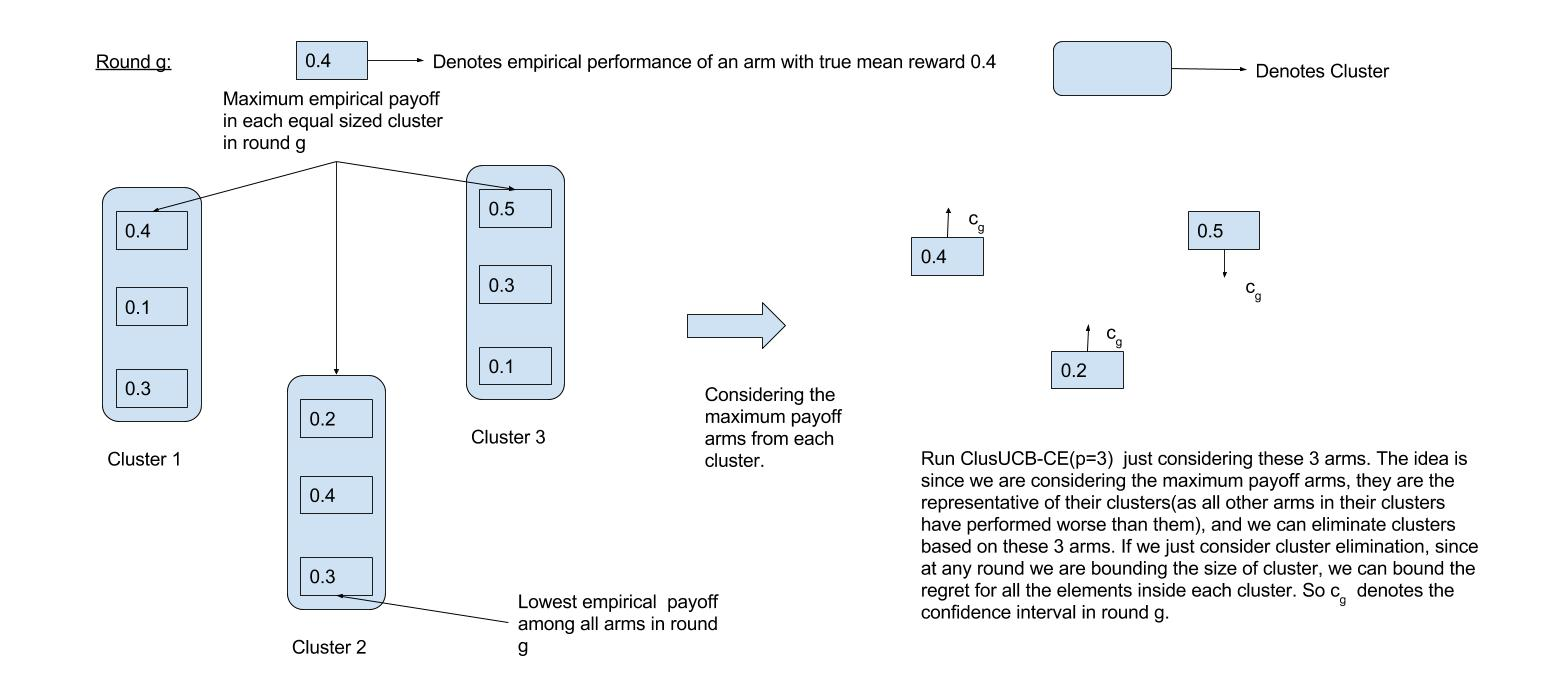
\includegraphics[scale=0.3]{img/diagCluster.jpg}
\caption{Cluster Elimination}
\label{Fig:ClusFig}
\end{figure}

%\begin{proposition}
%Considering only the cluster elimination condition and $p>1$, the total regret till $T$ is upper bounded by $\E [R_{T}]\leq \sum\limits_{i\in A:\Delta_{i}\geq b}\bigg\lbrace \bigg(\dfrac{2^{2+4\rho_{s}}\rho_{s}^{2\rho_{s}}T^{1-\rho_{s}}}{\psi^{\rho_{s}}\Delta_{i}^{4\rho_{s}-1}}\bigg) + \bigg(\Delta_{i}+\dfrac{32\rho_{s}\log{(\psi T\dfrac{\Delta_{i}^{4}}{16\rho_{s}^{2}})}}{\Delta_{i}}\bigg)  +  \bigg(\dfrac{T^{1-\rho_{s}}\rho_{s}^{2\rho_{s}}2^{2\rho_{s}+3}}{\psi^{\rho_{s}}\Delta_{i}^{4\rho_{s} -1}} \bigg)\bigg \rbrace +\sum\limits_{i\in A:0\leq\Delta_{i}\leq b}\bigg(\dfrac{T^{1-\rho_{s}}\rho_{s}^{2\rho_{s}}2^{2\rho_{s}+3}}{\psi^{\rho_{s}}b^{4\rho_{s} -1}} \bigg) + max_{i:\Delta_{i}\leq b}\Delta_{i}T$ for all $b\geq \sqrt{\dfrac{e}{T}}$, where $\rho_{s}\in (0,1]$ is the cluster elimination parameter, $\psi$ is the exploration regulatory factor, $p$ is the number of clusters and $T$ is the horizon.
%\end{proposition}

An illustrative diagram explaining Cluster Elimination is given in \textbf{Figure \ref{Fig:ClusFig}}. A slight modification to the algorithm allows us to do cluster elimination without any arm elimination. By taking $p>1$, removing the arm elimination condition, stopping when we are just left with one cluster and pulling the $max\lbrace \hat{r}_{i}\rbrace$, where ${i}\in B_{m}$ we can achieve this. We also take $\rho_{s}\in (0,1]$ as a constant in this proof whereby in Corollary \ref{Result:Corollary:1} and \ref{Result:Corollary:2} we use the different definitions. The theoretical analysis remains same as we have always bounded the values of $\rho_{s}\in (0,1]$.
 

\begin{proof}
% A sketch of the proof is given below,
%
%\begin{itemize}
%\item Define $C_{g}$ as the active cluster set which contains the max payoff arm from all the clusters active in the $g$-th round. So, the maximum cardinality of $C_{g}$ is $p$ and also this is always a non-increasing set.
%\item Now, the elements in $C_{g}$ which are the max-payoff arm from each cluster(if there are more than $1$ max-payoff arm in a cluster then choose randomly between them) are not fixed and hence like $B_{m}$ in proposition \ref{proofTheorem:Prop:1} cannot be tied to an arm $a_{i}$ throughout the rounds. For this purpose the $i$-th element in $C_{g}$ we tie to a cluster, that is $a_{\max_{s_{k}}}\in C_{g}$ is the max payoff arm in the cluster $s_{k}$ if the cluster $s_{k}$ still surviving in round $g$ and call $a_{\max_{s_{k}}}$ as a cluster arm. 
%\item Define $g$-th round(like in proposition \ref{proofTheorem:Prop:1}) as the same way as the $m$-th round signifying the first/minimum round when a cluster gets eliminated.
%%\item Let in the $g$-th round $C_{g}$ be the set which contains all the max payoff arms from each cluster.
%\item For regret bound proof according to proposition \ref{proofTheorem:Prop:1}, consider only this $C_{g}$ and proof following the same way as in proposition \ref{proofTheorem:Prop:1} with some changes. In any round $g$, atleast one of these $5$ events must occur:-
%\begin{itemize}
%\item \textbf{Case a1:} $a^{*}\in C_{g}$ and bound the regret that a sub-optimal cluster arm $a_{\max_{s_{k}}}\in C_{g}$ does not get eliminated on or before $g_{s_{k}}$-th round.
%\item \textbf{Case a2:} $a^{*}\notin C_{g}$ and bound the regret that a sub-optimal cluster arm $a_{\max_{s_{k}}}$ does not get eliminated on or before $a_{max_{s^{*}}}\in C_{g}$, such that $a_{\max_{s^{*}}},a^{*}\in s^{*}$ and $a_{\max_{s^{*}}}\neq a^{*}$. So, $a^{*}$ survives by this condition.
%\item \textbf{Case b1:} Cluster arm $a_{s_{k}}$ gets eliminated on $g_{s_{k}}$-th round(or before) with $a^{*}$ still in $B_{g_{s_{k}}}$ and calculate the regret for the arm pulls for all arms in cluster $s_{k}$(clusters are fixed).
%\item \textbf{Case b2:} $a^{*}\in C_{g}$ and $s^{*}$ gets eliminated by another sub-optimal cluster arm and bound this regret.
%\item \textbf{Case b3:} $a^{*}\notin C_{g}$ and $s^{*}$ gets eliminated by another sub-optimal cluster arm  and bound this regret.
%\end{itemize}
%For bounding the regret we use Chernoff-Hoeffding bound and use it on the current set of cluster arms $a_{max_{s_{k}}}\in C_{g},\forall s_{k}\in S$. This will work because of the algorithm, we are pulling all the  surviving arms equal number of times in each round and applying the same confidence interval for cluster elimination to all of the elements of $C_{g}$ and also we fix the clusters from beginning of the rounds.
%%Hence, $C_{g}$ actually behaves like the set $B_{m}$ in proposition $5$ but contains just the max payoff arm from each cluster.
%\item Introduce a constant $\rho_{s}\in (0,1]$ for cluster elimination to mimic the arm elimination condition in proposition \ref{proofTheorem:Prop:1}, but with the condition that whenever $\sqrt{\rho_{s}\epsilon_{g_{s_{k}}}} <  \dfrac{\Delta_{a_{\max_{s_{k}}}}}{2}, a_{\max_{s_{k}}}\in C_{g}$, then the cluster $s_{k}$(where 
%$\hat{r}_{a_{\max_{s_{k}}}}$ is the max payoff) gets eliminated. Because of the algorithm, we are guaranteed that the  maximum size of the cluster in the $g$-th round is $\ell=\bigg\lceil \dfrac{K}{p}\bigg\rceil$.
%\end{itemize}

Let $C_{g_{s_{k}}}=\lbrace \hat{r}_{a_{\max_{s_{k}}}} | \forall s_{k}\in S \rbrace$, that is let $C_{g_{s_{k}}}$ be the set of all arms which has the maximum estimated payoff arms from their respective clusters in the $g_{s_{k}}$-th round.  
Let, for each sub-optimal cluster arm $a_{\max_{s_{k}}}\in C_{g_{s_{k}}}$, $g_{s_{k}}=\min{\lbrace g|\sqrt{\rho_{s}\epsilon_{g}} < \dfrac{\Delta_{a_{\max_{s_{k}}}}}{2} \rbrace}$. So, $g_{s_{k}}$ be the first round when $\sqrt{\rho_{s}\epsilon_{g_{s_{k}}}} < \dfrac{\Delta_{a_{\max_{s_{k}}}}}{2}$ where $a_{\max_{s_{k}}}\in C_{g_{s_{k}}}$ is the maximum payoff arm in cluster $s_{k}$. Here, $a_{\max_{s_{k}}}$ is called cluster arm. Here, $A_{{s_{k}}}$ denotes the arm set in the cluster $s_{k}$. Let $A_{s_{k}}^{'}=\lbrace i\in A_{s_{k}}: \Delta_{i}> b\rbrace$, $A_{s_{k}}^{''}=\lbrace i\in A_{s_{k}}: \Delta_{i} > 0\rbrace$, $A^{'}=\lbrace i\in A: \Delta_{i}> b\rbrace$ and $A^{''}=\lbrace i\in A: \Delta_{i} > 0\rbrace$.

%The parameter $\rho_{s}$ is introduced just to make sure that the cluster elimination is a more aggressive elimination than arm elimination.
\subsection*{Case a: \textit{ Some sub-optimal cluster arm $a_{max_{s_{k}}}$ is not eliminated in round $g_{s_{k}}$ or before with $* \in C_{g_{s_{k}}}$ }}
%\subsubsection*{Case a1: \textit{ Some sub-optimal cluster arm $a_{max_{s_{k}}}$ is not eliminated in round $g_{s_{k}}$ or before and the optimal cluster arm $a^{*}\in C_{g_{s_{k}}} \subset B_{m}$ }}

%	In arm elimination condition, given the choice of confidence interval $c_{g_{s_{k}}}=\sqrt{\dfrac{\rho_{s} \log (\psi T\epsilon_{g_{s_{k}}}^{2})}{2 n_{g_{s_{k}}}}}$, we want to bound the probability of the event $\hat{r}_{s_{k}}+c_{g_{s_{k}}}\geq \hat{r}^{*}-c_{g_{s_{k}}}$.
%with a more tighter event of $ \hat{r}_{i} + \sqrt{w_{s_{k}}}c_{m} \leq \hat{r}^{*} - \sqrt{w_{s_{k}}}c_{m}$ which will result in faster elimination of arms within a cluster, given the choice of $c_{m}$ and $w_{s_{k}}$.
  %Now, $c_{g_{s_{k}}}=\sqrt{\dfrac{\rho_{s} \log (\psi T\epsilon_{g_{s_{k}}}^{2})}{2 n_{g_{s_{k}}}}}$, where $0 < \rho_{s}\leq 1$.
  
	Following the steps of Theorem \ref{Result:Theorem:1} Case $a2$, an arbitrary sub-optimal arm ${i}\in A^{'}$ can get eliminated only when the event,
	\begin{align}
	\hat{r}_{a_{\max_{s_{k}}}}  \le r_{a_{\max_{s_{k}}}} + c_{m_{i}} \text{ and } \label{eq:appB:armelim-casea}
 	\hat{r}^{*}\geq  r^{*} - c_{m_{i}}
	\end{align}
	
	takes place. So to bound the regret we need to bound the probability of the complementary event of these two conditions.  
  
  
  Putting the value of $n_{g_{s_{k}}}=\dfrac{2\log{(\psi T\epsilon_{g_{s_{k}}}^{2})}}{\epsilon_{g_{s_{k}}}}$ in $c_{g_{s_{k}}}$ we get,
  \begin{align*}
  c_{g_{s_{k}}}= & \sqrt{\dfrac{\rho_{s}*\epsilon_{g_{s_{k}}}\log (\psi  T\epsilon_{g_{s_{k}}}^{2})}{2*2 \log(\psi T\epsilon_{g_{s_{k}}}^{2})}}\\
  &=\sqrt{\dfrac{\rho_{s}\epsilon_{g_{s_{k}}}}{2}}\\
  &=\sqrt{\rho_{s}\epsilon_{g_{s_{k}}+1}} < \dfrac{\sqrt{\rho_{s}}\Delta_{a_{\max_{s_{k}}}}}{4} < \dfrac{\Delta_{a_{\max_{s_{k}}}}}{4}
  \end{align*}
%  $c_{g_{s_{k}}}=\sqrt{\dfrac{\rho_{s}*\epsilon_{g_{s_{k}}}\log (\psi T\epsilon_{g_{s_{k}}}^{2})}{2*2 \log(\psi T\epsilon_{g_{s_{k}}}^{2})}}=\sqrt{\dfrac{\rho_{s}\epsilon_{g_{s_{k}}}}{2}} = \sqrt{\rho_{s}\epsilon_{g_{s_{k}}+1}} < \dfrac{\sqrt{\rho_{s}}\Delta_{a_{max_{s_{k}}}}}{4} < \dfrac{\Delta_{a_{max_{s_{k}}}}}{4} $

  Again, for $a_{\max_{s_{k}}}, * \in C_{g_{s_{k}}}$, 
  \begin{align*}
  \hat{r}_{a_{\max_{s_{k}}}} + c_{g_{s_{k}}}\leq r_{a_{\max_{s_{k}}}} + 2c_{g_{s_{k}}} &= \hat{r}_{a_{\max_{s_{k}}}} + 4c_{g_{k}} - 2c_{g_{s_{k}}}\\
  &< r_{a_{\max_{s_{k}}}} + \Delta_{a_{\max_{s_{k}}}} - 2c_{g_{s_{k}}}\\
  &= r^{*} -2c_{g_{s_{k}}}\\
  &\leq \hat{r}^{*} - c_{g_{s_{k}}}
  \end{align*}
   
%Hence, we get that as soon as $\sqrt{\rho_{s}\epsilon_{g_{s_{k}}}}<\dfrac{\Delta_{a_{max_{s_{k}}}}}{2}$, 
% 	$a_{max_{s_{k}}}\in C_{g_{s_{k}}}$ gets eliminated.
%  So, $\hat{r}_{i}+c_{m}\leq \hat{r}_{i}+2c_{m}\leq r_{i} + \Delta_{i} - 2\sqrt{w_{s_{k}}}c_{m}\leq r^{*} - 2\sqrt{w_{s_{k}}}c_{m}$
%\leq \hat{r}^{*} - \sqrt{w}c_{m}
%  $\Rightarrow\hat{r}_{i}+c_{m}\leq \hat{r}_{i} - \sqrt{w}c_{m}  \leq r^{*} - \sqrt{w}c_{m}$
%  $\Rightarrow \hat{r}_{i} \leq {r}^{*} - 2\sqrt{w_{s_{k}}}c_{m} - 2c_{m} \leq \hat{r}^{*} - 2\sqrt{w_{s_{k}}}c_{m}$
%	So, we need to bound the probability of the event of $\hat{r}_{a_{max_{s_{k}}}}+c_{g_{s_{k}}}\geq \hat{r}^{*}-c_{g_{s_{k}}}$.
  %given that $\sqrt{\rho_{s}\epsilon_{g_{s_{k}}}}<\dfrac{\Delta_{a_{max_{s_{k}}}}}{2}$ becomes true for some arm $a_{max_{s_{k}}}\in C_{g_{s_{k}}}$ after the $g$-th round and $c_{g_{s_{k}}}=\sqrt{\dfrac{\rho_{s} \log (\psi T\epsilon_{g_{s_{k}}}^{2})}{2 n_{g_{s_{k}}}}}$.
%  $\Rightarrow \hat{r}_{i}+2c_{m}\leq \hat{r}_{i} + 2\sqrt{w}c_{m} \leq \hat{r}^{*}$
%  $\Rightarrow \hat{r}_{i} + \sqrt{w}c_{m} \leq \hat{r}^{*} - \sqrt{w}c_{m}$
%  $\Rightarrow\hat{r}_{i}+c_{m}\sqrt{\dfrac{w\ell_{m}}{\epsilon_{m}}} \leq \hat{r}^{*}-c_{m}\sqrt{\dfrac{w\ell_{m}}{\epsilon_{m}}} $, as $c_{m}\sqrt{\dfrac{w\ell_{m}}{\epsilon_{m}}} > 0$

%\begin{proof} of Proposition 2:
% 
%Now, we can bound $\hat{r}_{i}+c_{m}\leq \hat{r}^{*}-c_{m}$ given that $\sqrt{\epsilon_{m}}<\dfrac{\Delta_{i}}{2}$ for some arm $a_{i}\in s_{k}$. 
%	So, we need to bound the probability,
%	\begin{align*}
%	&\mathbb{P}\lbrace\hat{r}^{*}\leq r^{*} - c_{g_{s_{k}}}\rbrace\leq U_{g}\text{, where $U_{g}$ is an  arbitrary upper bound.}
%	\end{align*}

	Applying Chernoff-Hoeffding bound and considering independence of complementary of the two events in \ref{eq:appB:armelim-casea},
 
 \begin{align*}
 \mathbb{P}\bigg\lbrace\hat{r}^{*} \leq r^{*} - c_{g_{s_{k}}}\bigg\rbrace&\leq exp(-2c_{g_{s_{k}}}^{2}n_{g_{s_{k}}})\\
 &\leq exp(-2 * \dfrac{\rho_{s}\log ( \psi T\epsilon_{g_{s_{k}}}^{2})}{2 n_{g_{s_{k}}}} *n_{g_{s_{k}}})\\
 &\leq \dfrac{1}{(\psi T\epsilon_{g_{k}}^{2})^{\rho_{s}}}
 \end{align*}
% \hspace*{0em} $\mathbb{P}\lbrace\hat{r}^{*}\leq r^{*} - c_{g_{s_{k}}}\rbrace\leq exp(-2c_{g_{s_{k}}}^{2}n_{g_{s_{k}}})$
% \hspace*{8em} $\leq exp(-2 * \dfrac{\rho_{s}\log ( \psi T\epsilon_{g_{s_{k}}}^{2})}{2 n_{g_{s_{k}}}} *n_{g_{s_{k}}})$
% \hspace*{8em} $\leq \dfrac{1}{(\psi T\epsilon_{g_{k}}^{2})^{\rho_{s}}}$

 
Similarly, $\mathbb{P}\bigg\lbrace\hat{r}_{a_{max_{s_{k}}}}\geq r_{a_{max_{s_{k}}}} + c_{g_{s_{k}}}\bigg\rbrace\leq \dfrac{1}{(\psi T\epsilon_{g_{s_{k}}}^{2})^{\rho_{s}}}$
 
Summing, the two up, the probability that a sub-optimal cluster arm $a_{max_{s_{k}}}\in C_{g_{s_{k}}}$ is not eliminated in $g_{s_{k}}$-th round is  $\bigg(\dfrac{2}{(\psi  T\epsilon_{g_{s_{k}}}^{2})^{\rho_{s}}}\bigg)$. 
  Now, for each round $g_{s_{k}}$, all the elements of $C_{g_{s_{k}}}$ are the respective max payoff arms of their cluster $s_{k}$, that is all the other arms in their respective clusters have performed worse than them. Hence, since $A_{s_{k}}^{'}\supset C_{g_{s_{k}}}$, we are pulling all the surviving arms equally in each round and since clusters are fixed so we can bound the maximum probability that a sub-optimal arm ${j}\in A^{'}_{s_{k}}$  and ${j}\in s_{k}$ such that $a_{max_{s_{k}}}\in C_{g_{s_{k}}}$ is not eliminated on or before the $g_{s_{k}}$-th round by the same probability of 
  
  %, \forall s_{k}\in S_{g_{s_{k}}}
\begin{align*}
\bigg(\dfrac{2}{(\psi T\epsilon_{g_{s_{k}}}^{2})^{\rho_{s}}}\bigg)
\end{align*}  
 
 
Summing up over all arms in $s_{k}$ and bounding the regret trivially by $T\Delta_{i}$,
\begin{align*}
\sum_{i\in A_{s_{k}}^{'}}\bigg(\dfrac{2T\Delta_{i}}{(\psi T\epsilon_{g_{s_{k}}}^{2})^{\rho_{s}}}\bigg)
\end{align*}

 
Summing up over all $p$ clusters and bounding the regret for each arm $i\in A_{s_{k}}^{'} $ trivially by $T\Delta_{i}$,
 \begin{align*}
 \sum_{k=1}^{p}\sum_{i\in A_{s_{k}}^{'}}\bigg(\dfrac{2T\Delta_{i}}{(\psi T\dfrac{\Delta_{i}^{4}}{16\rho_{s}^{2}})^{\rho_{s}}}\bigg) &= \sum_{i\in A^{'}}\bigg(\dfrac{2T\Delta_{i}}{(\psi  T\dfrac{\Delta_{i}^{4}}{16\rho_{s}^{2}})^{\rho_{s}}}\bigg) \\
 &\leq \sum_{i\in A^{'}}\bigg(\dfrac{2^{1+4\rho_{s}}T^{1-\rho_{s}}\rho_{s}^{2\rho_{s}}\Delta_{i}}{\psi^{\rho_{s}}\Delta_{i}^{4\rho_{s}}}\bigg)\\
 &\leq \sum_{i\in A^{'}}\bigg(\dfrac{2^{1+4\rho_{s}}\rho_{s}^{2\rho_{s}}T^{1-\rho_{s}}}{\psi^{\rho_{s}}\Delta_{i}^{4\rho_{s}-1}}\bigg)\\
 &= \sum_{i\in A^{'}}\bigg(\dfrac{C_{1}(\rho_{s})T^{1-\rho_{s}}}{\Delta_{i}^{4\rho_{s}-1}}\bigg) \text{, where } C_1(x) = \frac{2^{1+4x}x^{2x}}{\psi^{x}}
 \end{align*}
 
% \hspace*{4em} $\sum_{k=1}^{p}\sum_{i\in A_{s_{k}}}\bigg(\dfrac{2T\Delta_{i}}{(\psi T\dfrac{\Delta_{i}^{4}}{16\rho_{s}^{2}})^{\rho_{s}}}\bigg)$
% \hspace*{4em} $\sum_{i\in A}\bigg(\dfrac{2T\Delta_{i}}{(\psi T\dfrac{\Delta_{i}^{4}}{16\rho_{s}^{2}})^{\rho_{s}}}\bigg)\leq \sum_{i\in A}\bigg(\dfrac{2^{1+4\rho_{s}}T^{1-\rho_{s}}\rho_{s}^{2\rho_{s}}\Delta_{i}}{\psi^{\rho_{s}}\Delta_{i}^{4\rho_{s}}}\bigg)$
% \hspace*{14em}
%$\leq \sum_{i\in A}\bigg(\dfrac{2^{1+4\rho_{s}}\rho_{s}^{2\rho_{s}}T^{1-\rho_{s}}}{\psi^{\rho_{s}}\Delta_{i}^{4\rho_{s}-1}}\bigg)$

%\subsubsection*{Case a2: \textit{ Some sub-optimal cluster arm $a_{max_{s_{k}}}$ is not eliminated in round $g_{s_{k}}$ or before and the optimal cluster arm $a^{*}\notin C_{g_{s_{k}}} \subset B_{m}$ }}
%%\textbf{Case a2:} Some sub-optimal cluster arm $a_{max_{s_{k}}}$ is not eliminated in round $g_{s_{k}}$ or before and the optimal cluster arm $a^{*}\notin C_{g_{s_{k}}} \subset B_{m}$. 
%	
%	In the above case we considered that $a^{*}\in C_{g_{s_{k}}}$ being the max-payoff arm from optimal cluster $s^{*}$. Now, if that is not the case and $\exists a_{\max_{s^{*}}}\in s^{*}$ such that $\hat{r}_{a_{\max_{s^{*}}}}> \hat{r}^{*}$, so $a_{\max_{s^{*}}}$ will be in $C_{g_{s_{k}}}$ in the $g_{s_{k}}$-th round. In this case for some sub-optimal arm $a_{max_{s_{k}}}\in C_{g_{s_{k}}}$, we have to bound the probability
%	\begin{align*}
%	&\mathbb{P}\bigg\lbrace\hat{r}_{a_{\max_{s_{k}}}}+c_{g_{s_{k}}}\bigg\rbrace< \mathbb{P}\bigg\lbrace\hat{r}_{a_{\max_{s^{*}}}}-c_{g_{s_{k}}}\bigg\rbrace
%	\end{align*}		 
%	 
%	 
%	 But, this probability can be no worse than case a1 since $r_{\max_{s^{*}}} < r^{*}$ and all arms get pulled $n_{g_{s_{k}}}$ number of times in the $g$-th round. So the regret for not eliminating a sub-optimal cluster even when $a^{*}\notin C_{g_{s_{k}}}$(but still surviving in $s^{*}$) can be no worse than,
%	 \begin{align*} 
%	 \bigg(\dfrac{2}{(T\epsilon_{g_{s_{k}}}^{2})^{\rho_{s}}}\bigg) 
%	 \end{align*}
%	 After summing over all arms in $A$ and bounding 
%trivially by $T\Delta_{i}$ we get the same result as above we can show that the regret can be no more than,
% \begin{align*}
% &\sum_{i\in A^{'}}\bigg(\dfrac{2^{1+4\rho_{s}}\rho_{s}^{2\rho_{s}}T^{1-\rho_{s}}}{\psi^{\rho_{s}}\Delta_{i}^{4\rho_{s}-1}}\bigg)=\sum_{i\in A^{'}}\bigg(\dfrac{C_{1}(\rho_{s})T^{1-\rho_{s}}}{\Delta_{i}^{4\rho_{s}-1}}\bigg)
% \end{align*}
%%$\sum_{i\in A}\bigg(\dfrac{2^{1+4\rho_{s}}\rho_{s}^{2\rho_{s}}T^{1-\rho_{s}}}{\psi^{\rho_{s}}\Delta_{i}^{4\rho_{s}-1}}\bigg)$


\subsection*{Case b: \textit{For each arm $i$, either ${i}$ is eliminated in round $g_{s_{k}}$ or before or there is no optimal arm ${*}$ in $C_{g_{s_{k}}}$ }}

\subsubsection*{Case b1: \textit{${*}\in C_{g_{s_{k}}}$ for each arm $i \in A'$ and cluster $s_{k}$ eliminated on or before $g_{s_{k}}$} }
	
	Again, in the $g_{s_{k}}$-th round, the maximum total elements in the cluster $s_{k}$ can be no more than $\ell=\bigg\lceil \dfrac{K}{p}\bigg\rceil$.
 
Also, since we are eliminating a sub-optimal cluster arm $a_{\max_{s_{k}}}\in C_{g_{s_{k}}}$ on or before round $g_{s_{k}}$, it is pulled (along with all the other arms in that cluster) no longer than,
 \begin{align*}
 &n_{g_{s_{k}}}=\bigg\lceil\dfrac{2\log{(\psi T\epsilon_{g_{s_{k}}}^{2})}}{\epsilon_{g_{s_{k}}}}\bigg\rceil
 \end{align*}

So, the total contribution of $a_{\max_{s_{k}}}$  along with all the other arms in the cluster till round $g_{s_{k}}$ is given by,
 \begin{align*}
 &\sum_{i\in A_{s_{k}}}\Delta_{i}\bigg\lceil\dfrac{2\log{(\psi T\epsilon_{g_{s_{k}}}^{2})}}{\epsilon_{g_{s_{k}}}}\bigg\rceil\\
 &\leq\sum_{i\in A_{s_{k}}^{'}}\Delta_{i}\bigg\lceil\dfrac{2\log{(\psi T(\dfrac{\Delta_{i}}{2\sqrt{\rho_{s}}})^{4})}}{(\dfrac{\Delta_{i}}{2\sqrt{\rho_{s}}})^{2}}\bigg\rceil \text{, since }\sqrt{\rho_{s}\epsilon_{g_{s_{k}}}} <\dfrac{\Delta_{a_{max_{s_{k}}}}}{2} <  \dfrac{\Delta_{i}}{2} \text{, as } {r}_{a_{max_{s_{k}}}}>{r}_{i},\forall i\in s_{k}\\
 &\leq\sum_{i\in A_{s_{k}}^{'}}\Delta_{i}\bigg(1+\dfrac{32*\rho_{s}*\log{(\psi T(\dfrac{\Delta_{i}}{2\sqrt{\rho_{s}}})^{4})}}{\Delta_{i}^{2}}\bigg)\\
 &\leq\sum_{i\in A_{s_{k}}^{'}}\Delta_{i}\bigg(1+\dfrac{32\rho_{s}\log{(\psi T\dfrac{\Delta_{i}^{4}}{16\rho_{s}^{2}})}}{\Delta_{i}^{2}}\bigg)
 \end{align*}

 
Summing over all $p$ clusters the total regret is given by,
 
\begin{align*}
&\sum_{k=1}^{p}\sum_{i\in A_{s_{k}}^{'}}\Delta_{i}\bigg(1+\dfrac{32\rho_{s}\log{(\psi  T\dfrac{\Delta_{i}^{4}}{16\rho_{s}^{2}})}}{\Delta_{i}^{2}}\bigg)\\
&\leq\sum_{i\in A^{'}}\Delta_{i}\bigg(1+\dfrac{32\rho_{s}\log{(\psi T\dfrac{\Delta_{i}^{4}}{16\rho_{s}^{2}}})}{\Delta_{i}^{2}}\bigg)
\end{align*}


\subsubsection*{Case b2: \textit{$s^{*}$ is eliminated by some sub-optimal cluster.} } 
	
	Let $C_{g}^{'}=\lbrace a_{max_{s_{k}}}\in A^{'}|\forall s_{k}\in S \rbrace$ and $C_{g}^{''}=\lbrace a_{max_{s_{k}}}\in A^{''}|\forall s_{k}\in S \rbrace$. Firstly, if conditions of case $b1$ holds then the optimal arm ${*}\in C_{g_{s_{k}}}$ will not be eliminated in round $g_{s_{k}}=g_{*}$ or it will lead to the contradiction that $r_{a_{\max_{s_{k}}}}>r^{*}$ where $a_{\max_{s_{k}}},{*}\in C_{g_{s_{k}}}$. In any round $g_{*}$, if the optimal arm ${*}$ gets eliminated then for any round from $1$ to $g_{s_{j}}$ all arms $a_{\max_{s_{j}}}\in C_{g_{s_{k}}},\forall s_{j}\neq s^{*}$ such that $g_{s_{j}}< g_{*}$ were eliminated according to assumption in Case $a$. Let, the arms surviving till $g_{*}$ round be denoted by $C_{g}^{'}$. This leaves any arm $a_{s_{b}}$ such that $g_{s_{b}}\geq g_{*}$ to still survive and eliminate arm ${*}$ in round $g_{*}$. Let, such arms that survive ${*}$ belong to $C_{g}^{''}$. Also maximal regret per step after eliminating ${*}$ is the maximal $\Delta_{a_{\max_{s_{j}}}}$ among the remaining arms ${a_{\max_{s_{j}}}}\in C_{g_{s_{j}}}$ with $g_{s_{j}}\geq g_{*}$. Hence, the maximal regret after eliminating the arm ${*}$ is upper bounded by, 
 \begin{align*}
 &\sum_{g_{*}=0}^{max_{a_{\max_{s_{j}}}\in C_{g}^{'}}g_{s_{j}}}\sum_{\substack{a_{\max_{s_{k}}}\in C_{g}^{''}: \\ g_{s_{k}} \geq g_{*}}}\bigg(\dfrac{2}{(\psi T\epsilon_{g_{s^{*}}}^{2})^{\rho_{s}}} \bigg).T\max_{\substack{a_{\max_{s_{j}}}\in C_{g}^{''}: \\ g_{s_{j}}\geq g_{*}}}{\Delta}_{a_{\max_{s_{j}}}}
 \end{align*}
%Let $g_{s_{b}}=\min\lbrace g|\sqrt{\rho_{s}\epsilon_{g}}<\dfrac{\Delta_{a_{\max_{s_{b}}}}}{2}\rbrace$.
But, we know that for any round $g$, elements of $C_{g}$ are the best performers in their respective clusters. So, taking that into account and $A'\supset C_{g}^{'}$ and $A''\supset C_{g}^{''}$ the regret can be bounded by,
%\text{, since }\sqrt{\rho_{s}\epsilon_{g_{s_{j}}}} < \dfrac{\Delta_{j}}{2} <  \dfrac{\Delta_{j}}{2} \text{, as }{r}_{a_{s_{j}}}>{r}_{j},\forall j\in s_{j}
\begin{align*}
 & \sum_{g_{*}=0}^{max_{j\in A^{'}}g_{s_{j}}}\sum_{i\in A^{''}:g_{s_{k}}>g_{*}}\bigg(\dfrac{2}{(\psi T\epsilon_{g_{s_{k}}}^{2})^{\rho_{s}}} \bigg).T\max_{j\in A^{''}:g_{s_{j}}\geq g_{*}}{\Delta}_{j}\\
 &\leq\sum_{g_{*}=0}^{max_{j\in A^{'}}g_{s_{j}}}\sum_{i\in A^{''}:g_{s_{k}}>g_{*}}\bigg(\dfrac{2}{(\psi T\epsilon_{g_{s_{k}}}^{2})^{\rho_{s}}} \bigg).T.2\sqrt{\rho_{s}\epsilon_{g_{s_{j}}}}\\
 &\leq\sum_{g_{*}=0}^{max_{j\in A^{'}}g_{s_{j}}}\sum_{i\in A^{''}:g_{s_{k}}>g_{*}}\bigg(\dfrac{4T^{1-\rho_{s}}}{\psi^{\rho_{s}}\epsilon_{g_{s_{k}}}^{2\rho_{s} - \frac{1}{2}}} \bigg)\\
 &\leq\sum_{i\in A^{''}:g_{s_{k}}>g_{*}}\sum_{g_{*}=0}^{\min{\lbrace g_{s_{k}},g_{s_{b}}\rbrace}}\bigg(\dfrac{4T^{1-\rho_{s}}}{\psi^{\rho_{s}}2^{({2\rho_{s} - \frac{1}{2}})g_{*}}} \bigg) \\
 &\leq\sum_{i\in A^{'}}\bigg(\dfrac{4T^{1-\rho_{s}}}{\psi^{\rho_{s}}2^{({2\rho_{s} - \frac{1}{2}})g_{*}}} \bigg)+\sum_{i\in A^{''}\setminus A^{'}}\bigg(\dfrac{4T^{1-\rho_{s}}}{\psi^{\rho_{s}}2^{({2\rho_{s} - \frac{1}{2}})g_{s_{b}}}} \bigg)\\ 
 &\leq\sum_{i\in A^{'}}\bigg(\dfrac{4\rho_{s}^{2\rho_{s}}T^{1-\rho_{s}}*2^{2\rho_{s}-\frac{1}{2}}}{\psi^{\rho_{s}}\Delta_{i}^{4\rho_{s}-1}} \bigg)+\sum_{i\in A^{''}\setminus A^{'}}\bigg(\dfrac{4\rho_{s}^{2\rho_{s}}T^{1-\rho_{s}}*2^{2\rho_{s}-\frac{1}{2}}}{\psi^{\rho_{s}}b^{4\rho_{s}-1}} \bigg)\\
 &\leq\sum_{i\in A^{'}}\bigg(\dfrac{T^{1-\rho_{s}}\rho_{s}^{2\rho_{s}}2^{2\rho_{s}+\frac{3}{2}}}{\psi^{\rho_{s}}\Delta_{i}^{4\rho_{s}-1}} \bigg)+\sum_{i\in A^{''}\setminus A^{'}}\bigg(\dfrac{T^{1-\rho_{s}}\rho_{s}^{2\rho_{s}}2^{2\rho_{s}+\frac{3}{2}}}{\psi^{\rho_{s}}b^{4\rho_{s}-1}} \bigg)\\
 & = \sum_{i\in A^{'}}\bigg(\dfrac{C_{2}(\rho_{s})T^{1-\rho_{s}}}{\Delta_{i}^{4\rho_{s}-1}} \bigg)+\sum_{i\in A^{''}\setminus A^{'}}\bigg(\dfrac{C_{2}(\rho_{s})T^{1-\rho_{s}}}{b^{4\rho_{s}-1}} \bigg) \text{, where } C_2(x) = \frac{2^{2x+\frac{3}{2}}x^{2x}}{\psi^{x}}
\end{align*}

\subsubsection*{Case b3: \textit{${*}$ is not in $C_{g_{s_{k}}}$, but belongs to $B_{g_{s_{k}}}$} } 

In this case the optimal arm ${*}\in s^{*}$ is not eliminated, also $s^{*}$ is not eliminated. So, for all sub-optimal arms $i$ in $A'$ which gets eliminated on or before $g_{s_{k}}$ will get pulled no less than $\bigg\lceil\dfrac{2\log{(\psi T\epsilon_{g_{s_{k}}}^{2})}}{\epsilon_{g_{s_{k}}}}\bigg\rceil$ number of times, which leads to the following bound the contribution to the expected regret, as in Case $b1$:
% 
% \begin{align*}
%  &\sum_{i\in A^{'}}\Delta_{i}\bigg\lceil\dfrac{2\log{(\psi T\epsilon_{m_{i}}^{2})}}{\epsilon_{m_{i}}}\bigg\rceil
% \end{align*}
% Since $a^{*}$ is definitely in $B_{\max(m_{i},g_{s_{k}})}$ then following the same way as Case $b1$ we can show that can be no worse than,
\begin{align*}
 &\sum_{i\in A^{'}}\bigg\lbrace \Delta_{i}+\dfrac{32\rho_{s}\log{(\psi T\dfrac{\Delta_{i}^{4}}{16\rho_{s}^{2}})}}{\Delta_{i}} \bigg\rbrace 
\end{align*} 

%\subsubsection*{Case b3: \textit{Cluster $s^{*}$ containing the optimal arm ${*}$ is eliminated by a sub-optimal cluster and ${*}\notin C_{g}$}}
% 
%	Now, in the above case again we considered that ${*}$ is in $C_{g}$. In this case we will consider that the cluster $s^{*}$ containing the optimal arm ${*}$ was eliminated by another sub-optimal cluster and ${*}\notin C_{g}$. This will be the mirror case of Case $b2$ and since $s^{*}$ gets eliminated by $a_{s_{b}}$ such that $\sqrt{\rho_{s}\epsilon_{g_{s_{b}}}}\geq\dfrac{\Delta_{a_{s_{b}}}}{2}$ round $g_{*}$. Also maximal regret per step after eliminating ${*}$ is the maximal $\Delta_{j}$ among the remaining arms ${j}\in B_{m}$ with $g_{s_{j}}\geq g_{*}$. Following the same way above we can bound the regret as,
% 
%\begin{align*}
%&\sum_{i\in A^{'}}\bigg(\dfrac{T^{1-\rho_{s}}\rho_{s}^{2\rho_{s}}2^{2\rho_{s}+\frac{3}{2}}}{\psi^{\rho_{s}}\Delta_{i}^{4\rho_{s}-1}} \bigg)+\sum_{i\in A^{''}\setminus A^{'}}\bigg(\dfrac{T^{1-\rho_{s}}\rho_{s}^{2\rho_{s}}2^{2\rho_{s}+\frac{3}{2}}}{\psi^{\rho_{s}}b^{4\rho_{s}-1}} \bigg)\\
%& = \sum_{i\in A^{'}}\bigg(\dfrac{C_{2}(\rho_{s})T^{1-\rho_{s}}}{\Delta_{i}^{4\rho_{s}-1}} \bigg)+\sum_{i\in A^{''}\setminus A^{'}}\bigg(\dfrac{C_{2}(\rho_{s})T^{1-\rho_{s}}}{b^{4\rho_{s}-1}} \bigg)
%\end{align*}
 
Summing up \textbf{Case a} and \textbf{Case b}, the total regret till round $g$ is given by,
\begin{align*}
  R_{T} \leq &  \sum_{i\in A:\Delta_{i} > b}\bigg\lbrace\underbrace{\bigg(\dfrac{C_{1}(\rho_{s})T^{1-\rho_{s}}}{\Delta_{i}^{4\rho_{s}-1}}\bigg)}_{\text{case a}} + \underbrace{\bigg(2\Delta_{i}+\dfrac{64\rho_{s}\log{(\psi T\dfrac{\Delta_{i}^{4}}{16\rho_{s}^{2}})}}{\Delta_{i}} }_{\text{case b1+b3}} 
  \\&+ \underbrace{\bigg(\dfrac{C_{2}(\rho_{s})T^{1-\rho_{s}}}{\Delta_{i}^{4\rho_{s} -1}} \bigg)}_{\text{case b2}} \bigg\rbrace  + \underbrace{\sum_{i\in A:0\leq\Delta_{i}\leq b}\bigg(\dfrac{C_{2}(\rho_{s})T^{1-\rho_{s}}}{\Delta_{i}^{4\rho_{s} -1}} \bigg)}_{\text{case b2}}  + max_{i\in A:\Delta_{i}\leq b}\Delta_{i}T
\end{align*}

%R_{T} \leq &  \sum_{i\in A:\Delta_{i} > b}\bigg\lbrace\underbrace{\bigg(\dfrac{C_{1}(\rho_{s})T^{1-\rho_{s}}}{\Delta_{i}^{4\rho_{s}-1}}\bigg)}_{\text{case a}} + \underbrace{\bigg(2\Delta_{i}+\dfrac{32\rho_{s}\log{(\psi T\dfrac{\Delta_{i}^{4}}{16\rho_{s}^{2}})}}{\Delta_{i}} + \dfrac{32\rho_{a}\log{(\psi T\dfrac{\Delta_{i}^{4}}{16\rho_{a}^{2}})}}{\Delta_{i}}  \bigg) }_{\text{case b1+b3}} 
%  \\&+ \underbrace{\bigg(\dfrac{C_{2}(\rho_{s})T^{1-\rho_{s}}}{\Delta_{i}^{4\rho_{s} -1}} \bigg)}_{\text{case b2}} \bigg\rbrace  + \underbrace{\sum_{i\in A:0\leq\Delta_{i}\leq b}\bigg(\dfrac{C_{2}(\rho_{s})T^{1-\rho_{s}}}{\Delta_{i}^{4\rho_{s} -1}} \bigg)}_{\text{case b2}}  + max_{i:\Delta_{i}\leq b}\Delta_{i}T

%R_{T} \leq & \sum_{i\in A:\Delta_{i} > b}\bigg\lbrace\underbrace{\bigg(\dfrac{C_{1}(\rho_{s})T^{1-\rho_{s}}}{\Delta_{i}^{4\rho_{s}-1}}\bigg)}_{\text{case a1}} +  \underbrace{\bigg(\Delta_{i}+\dfrac{32\rho_{s}\log{(\psi T\dfrac{\Delta_{i}^{4}}{16\rho_{s}^{2}})}}{\Delta_{i}}\bigg)}_{\text{case b1}} \\
%	& + \underbrace{\bigg(\dfrac{C_{2}(\rho_{s})T^{1-\rho_{s}}}{\Delta_{i}^{4\rho_{s} -1}} \bigg)}_{\text{case b2}} 
%	+ \underbrace{\sum_{i\in A^{'}}\bigg\lbrace \Delta_{i}+\dfrac{32\rho_{a}\log{(\psi T\dfrac{\Delta_{i}^{4}}{16\rho_{a}^{2}})}}{\Delta_{i}} \bigg\rbrace}_{\text{case b3}}  + max_{i:\Delta_{i}\leq b}\Delta_{i}T\\
% \\& +\underbrace{\sum_{i\in A:0\leq\Delta_{i}\leq b}\bigg(\dfrac{2C_{2}(\rho_{s})T^{1-\rho_{s}}}{b^{4\rho_{s} -1}} \bigg)}_{\text{case b2+b3}}  
% \underbrace{\bigg(\dfrac{C_{2}(\rho_{s})T^{1-\rho_{s}}}{\Delta_{i}^{4\rho_{s} -1}} \bigg)}_{\text{case b3}}\bigg \rbrace+\underbrace{\sum_{i\in A:0\leq\Delta_{i}\leq b}\bigg(\dfrac{C_{2}(\rho_{s})T^{1-\rho_{s}}}{b^{4\rho_{s} -1}} \bigg)}_{\text{case b2}} \\
%    & + \underbrace{\sum_{i\in A:0\leq\Delta_{i}\leq b}\bigg(\dfrac{C_{2}(\rho_{s})T^{1-\rho_{s}}}{b^{4\rho_{s} -1}} \bigg)}_{\text{case b3}}
% \underbrace{\bigg(\dfrac{C_{1}(\rho_{s})T^{1-\rho_{s}}}{\Delta_{i}^{4\rho_{s}-1}}\bigg)}_{\text{case a2}} +
%  R_{T} \leq & \sum_{i\in A:\Delta_{i}\geq b}\bigg\lbrace\underbrace{\bigg(\dfrac{2^{1+4\rho_{s}}\rho_{s}^{2\rho_{s}}T^{1-\rho_{s}}}{\psi^{\rho_{s}}\Delta_{i}^{4\rho_{s}-1}}\bigg)}_{\text{case a1}} + \underbrace{\bigg(\dfrac{2^{1+4\rho_{s}}\rho_{s}^{2\rho_{s}}T^{1-\rho_{s}}}{\psi^{\rho_{s}}\Delta_{i}^{4\rho_{s}-1}}\bigg)}_{\text{case a2}} + \underbrace{\bigg(\Delta_{i}+\dfrac{32\rho_{s}\log{(\psi T\dfrac{\Delta_{i}^{4}}{16\rho_{s}^{2}})}}{\Delta_{i}}\bigg)}_{\text{case b1}} \\
%	& + \underbrace{\bigg(\dfrac{T^{1-\rho_{s}}\rho_{s}^{2\rho_{s}}2^{2\rho_{s}+\frac{3}{2}}}{\psi^{\rho_{s}}\Delta_{i}^{4\rho_{s} -1}} \bigg)}_{\text{case b2}} + \underbrace{\bigg(\dfrac{T^{1-\rho_{s}}\rho_{s}^{2\rho_{s}}2^{2\rho_{s}+\frac{3}{2}}}{\psi^{\rho_{s}}\Delta_{i}^{4\rho_{s} -1}} \bigg)}_{\text{case b3}}\bigg \rbrace+\underbrace{\sum_{i\in A:0\leq\Delta_{i}\leq b}\bigg(\dfrac{T^{1-\rho_{s}}\rho_{s}^{2\rho_{s}}2^{2\rho_{s}+\frac{3}{2}}}{\psi^{\rho_{s}}b^{4\rho_{s} -1}} \bigg)}_{\text{case b2}} \\
%   &	+ \underbrace{\sum_{i\in A:0\leq\Delta_{i}\leq b}\bigg(\dfrac{T^{1-\rho_{s}}\rho_{s}^{2\rho_{s}}2^{2\rho_{s}+\frac{3}{2}}}{\psi^{\rho_{s}}b^{4\rho_{s} -1}} \bigg)}_{\text{case b3}} + max_{i:\Delta_{i}\leq b}\Delta_{i}T\\
%  = & \sum\limits_{i\in A:\Delta_{i}\geq b}\bigg\lbrace\underbrace{\bigg(\dfrac{2^{2+4\rho_{s}}\rho_{s}^{2\rho_{s}}T^{1-\rho_{s}}}{\psi^{\rho_{s}}\Delta_{i}^{4\rho_{s}-1}}\bigg)}_{\text{case a1+a2}} + \underbrace{\bigg(\Delta_{i}+\dfrac{32\rho_{s}\log{(\psi T\dfrac{\Delta_{i}^{4}}{16\rho_{s}^{2}})}}{\Delta_{i}}\bigg)}_{\text{case b1}}  +  \underbrace{\bigg(\dfrac{T^{1-\rho_{s}}\rho_{s}^{2\rho_{s}}2^{2\rho_{s}+3}}{\psi^{\rho_{s}}\Delta_{i}^{4\rho_{s} -1}} \bigg)}_{\text{case b2+b3}}\bigg \rbrace \\
%  & +\underbrace{\sum\limits_{i\in A:0\leq\Delta_{i}\leq b}\bigg(\dfrac{T^{1-\rho_{s}}\rho_{s}^{2\rho_{s}}2^{2\rho_{s}+3}}{\psi^{\rho_{s}}b^{4\rho_{s} -1}} \bigg)}_{\text{case b2+b3}} + max_{i:\Delta_{i}\leq b}\Delta_{i}T  
  
  
\end{proof}





%\section{Proof of Theorem 1}
%\label{App:C}
%
%\begin{proof}
%The optimal cluster which contains $a^{*}$ is denoted by $s^{*}$. The subset of arms belonging to cluster $s_{k}$ is denoted by $A_{s_{k}}$ and similarly the subset of arms belonging to $s^{*}$ is denoted by $A_{s^{*}}$. Combining both the cases of Proposition \ref{proofTheorem:Prop:1} and Proposition \ref{proofTheorem:Prop:2} we can see that a sub-optimal arm $a_{i}$ can only be eliminated given that either $m_{i}$ or $g_{s_{k}}$s.t $\exists a_{i}\in s_{k}$ happens with $a^{*}\in s^{*}$ still surviving. In Proposition \ref{proofTheorem:Prop:1} we consider only arm elimination and in Proposition \ref{proofTheorem:Prop:2} we consider only cluster elimination. Also this proof we will consider $p>1$. So there will be slight modification from what we proved in proposition \ref{proofTheorem:Prop:1} with $p=1$. For random uniform allocation we will assume that each cluster $s_{k},\forall s_{k}\in S$, gets such an arm such that $r_{{max_{s_{k}}}}\geq r_{a_{i}},\forall i\in s_{k}$. Again, $r_{a^{*}}\geq r_{{max_{s_{k}}}}, \forall s_{k}\in S$. Here also we take $\rho_{a},\rho_{s}\in (0,1]$ as a constant in this proof whereby in Corollary \ref{Result:Corollary:1} and \ref{Result:Corollary:2} we use the different definitions. The theoretical analysis remains same as we have always bounded the values of $\rho_{a}\in (0,1]$(see Appendix \ref{App:E}). Let $A^{'}=\lbrace i \in A,\Delta_{i}> b\rbrace$ and $A^{''}=\lbrace i \in A,0 < \Delta_{i} \leq b\rbrace$. 
%%Also we cluster the arms based on $\epsilon_{m}$.
%% One vital point we point out is that, $\epsilon_{m}$(in proposition $3$) = $\epsilon_{g}$(in proposition $4$).
%\subsection*{Case a: \textit{Some sub-optimal arm $a_{i}$ is not eliminated in round $max(m_{i},g_{s_{k}})$ or before and the optimal arm $a^{*}\in B_{m_{i}}$}}
% 
%	In this case, we are looking at event of the maximum round till which atleast one of $m_{i}$ or $g_{s_{k}}$ did not happen. So, a sub-optimal arm $a_{i}$ cannot get eliminated in $4$ ways,
%\begin{enumerate}
%\item $a_{i}$ in $s^{*}$ and $m_{i}$ does not happen which is Proposition \ref{proofTheorem:Prop:1}, case $a1$.
%\item $a_{i}$ in $s_{k}$, where $r_{max_{s_{k}}}\leq r^{*}$ and $m_{i}$ does not happen. This case was not dealt in Proposition \ref{proofTheorem:Prop:1} as there we took $p=1$. Since, now $p>1$ and $r_{max_{s_{k}}}\leq r^{*}$, following the same way as case $a$, Proposition \ref{proofTheorem:Prop:1} we can show that the probability of $a_{i}$ not getting eliminated  cannot be worse than Proposition \ref{proofTheorem:Prop:1}, case $a1$ given that $\sqrt{\rho_{a}\epsilon_{m}}< \dfrac{\Delta^{'}_{i}}{2}$ where $\Delta^{'}_{i}=r_{max_{s_{k}}} - r_{i}\geq\Delta_{a_{max_{s_{k}}}}$ such that $r_{i}\in s_{k}$. Plugging in this $\Delta^{'}_{i}$ in Proposition \ref{proofTheorem:Prop:1}, case $a$ we can derive a similar bound where $\Delta^{'}_{i}\geq \Delta_{a_{max_{s_{k}}}}$ because otherwise $\sqrt{\epsilon_{m}\rho_{s}}< \dfrac{\Delta_{a_{max_{s_{k}}}}}{2}$ will happen and the cluster $s_{k}$ gets eliminated or $a_{max_{s_{k}}}$ will eliminate $a^{*}$ which is dealt later.
%\item $a_{i}\in s_{k}, a^{*}\in C_{g_{s_{k}}}$ and $g_{s_{k}}$ does not happen which is Proposition \ref{proofTheorem:Prop:2}, case $a1$.
%\item $a_{i}\in s_{k}, a^{*}\notin C_{g_{s_{k}}}$ and $g_{s_{k}}$ does not happen which is Proposition \ref{proofTheorem:Prop:2}, case $a2$.
%\end{enumerate}
%Taking summation of the events mentioned above($a1$-$a4$) gives us an upper bound on the regret given that the optimal arm $a^{*}$ is still surviving, 
%\begin{align*}
% &\underbrace{\sum_{i\in A_{s^{*}}}\bigg(\dfrac{C_{1}(\rho_{a})T^{1-\rho_{a}}}{\Delta_{i}^{4\rho_{a}-1}}\bigg)}_{\text{case a1}} + \underbrace{\sum_{i\in A\setminus A_{s^{*}}}\bigg(\dfrac{C_{1}(\rho_{a})T^{1-\rho_{a}}}{\Delta_{i}^{4\rho_{a}-1}}\bigg)}_{\text{case a2}} + \sum_{i\in A}\bigg\lbrace \underbrace{\bigg(\dfrac{2C_{1}(\rho_{s})T^{1-\rho_{s}}}{\psi^{\rho_{s}}\Delta_{i}^{4\rho_{s}-1}}\bigg)}_{\text{case a3+a4}}\bigg\rbrace \\
%& = \sum_{i\in A}\bigg\lbrace \bigg(\dfrac{C_{1}(\rho_{a})T^{1-\rho_{a}}}{\Delta_{i}^{4\rho_{a}-1}}\bigg) + \bigg(\dfrac{2C_{1}(\rho_{s})T^{1-\rho_{s}}}{\Delta_{i}^{4\rho_{s}-1}}\bigg)\bigg\rbrace
%\end{align*}
%
%%& = \sum_{i\in A}\bigg\lbrace \bigg(\dfrac{2^{1+4\rho_{s}}\rho_{s}^{2\rho_{s}}T^{1-\rho_{s}}}{\psi^{\rho_{a}}\Delta_{i}^{4\rho_{s}-1}}\bigg) + \bigg(\dfrac{2^{2+4\rho_{s}}\rho_{s}^{2\rho_{s}}T^{1-\rho_{s}}}{\psi^{\rho_{s}}\Delta_{i}^{4\rho_{s}-1}}\bigg)\bigg\rbrace
%
%
%\subsection*{Case b: \textit{Either an arm $a_{i}$ is eliminated in round $m_{i}$ or $g_{s_{k}}$ or before or else there is no optimal arm $a^{*}\in B_{m_{i}}$}} 
%
%\subsubsection*{Case b1: \textit{If an optimal arm $a^{*}\in B_{m_{i}}$ then the maximum pull of all arms $a_{i}\in A^{'}$}} 
% 
%	For any sub-optimal arm still surviving given $m_{i}$ or $g_{s_{k}}:a_{i}\in s_{k}$ have not happened and $a^{*}\in s^{*}$ still surviving then they get pulled $n_{m_{i}}$ or $n_{g_{s_{k}}}$ number of times(combining the result of Proposition \ref{proofTheorem:Prop:1} (case $b1$) and Proposition \ref{proofTheorem:Prop:2} (case $b1)$). Hence, we can show that till an arm or a cluster is eliminated, the maximum regret suffered due to pulling of a sub-optimal arm(or a sub-optimal cluster) is no less than,
% \begin{align*}
% &\sum_{i\in A^{'}}\bigg\lbrace\bigg(\Delta_{i}+\dfrac{32\rho_{a}\log{(\psi T\dfrac{\Delta_{i}^{4}}{16\rho_{a}^{2}})}}{\Delta_{i}}\bigg) + \bigg(\Delta_{i}+\dfrac{32\rho_{s}\log{(\psi T\dfrac{\Delta_{i}^{4}}{16\rho_{s}^{2}})}}{\Delta_{i}}\bigg)\bigg\rbrace 
% \end{align*}
%
% 
%\subsubsection*{Case b2: \textit{Optimal arm $a^{*}$ is eliminated by a sub-optimal arm}}
%  
%	Here, we take into consideration the error bound, that the optimal arm $a^{*}$ or the optimal cluster $s^{*}$ gets eliminated by any sub-optimal arm or sub-optimal cluster. This, can happen in $3$ ways,
%\begin{enumerate}
%\item In $s^{*}$, $a^{*}$ got eliminated by other arms surviving till $m_{*}$. Let, the arms surviving till $m_{*}$ round be denoted by $A^{'}_{s^{*}}$ such that $A^{'}_{s^{*}}=\lbrace i \in A_{s^{*}},\Delta_{i}> b\rbrace$. This leaves any arm $a_{b}$ such that $\sqrt{\rho_{a}\epsilon_{m}}\geq\dfrac{\Delta_{b}}{2}$ to still survive and eliminate arm $a^{*}$ in round $m_{*}$. Let, such arms that survive $a^{*}$ belong to $A^{''}_{s^{*}}$ such that $A^{''}_{s^{*}}=\lbrace i \in A_{s^{*}},0 < \Delta_{i} \leq b\rbrace$. As proved in Proposition \ref{proofTheorem:Prop:1}, case $b2$ this regret can be no more than,
% \begin{align*}
% &\sum_{i\in A^{'}_{s^{*}}}\bigg(\dfrac{C_{2}(\rho_{a})T^{1-\rho_{a}}}{\Delta_{i}^{4\rho_{a} -1}} \bigg)+\sum_{i\in A^{''}_{s^{*}}\setminus A^{'}_{s^{*}}}\bigg(\dfrac{C_{2}(\rho_{a})T^{1-\rho_{a}}}{b^{4\rho_{a} -1}} \bigg)
% \end{align*}
%We also see that here, we are concerned only within $s^{*}$ because of our assumption that there is only one $a^{*}\in A$ and clusters are fixed.
%\item $a^{*}\in C_{g}$ and $s^{*}$ gets eliminated by some other cluster. This is equivalent to Proposition \ref{proofTheorem:Prop:2}, case $b2$
%\item $a^{*}\notin C_{g}$ and $s^{*}$ gets eliminated by some other cluster. This is equivalent to Proposition \ref{proofTheorem:Prop:2}, case $b3$
%\end{enumerate} 
%
%
%Combining cases $b21$, $b22$ and $b23$ as mentioned above we can show,
% \begin{align*}
% &\underbrace{\sum_{i\in A^{'}_{s^{*}}}\bigg(\dfrac{C_{2}(\rho_{a})T^{1-\rho_{a}}}{\Delta_{i}^{4\rho_{a} -1}} \bigg)+\sum_{i\in A^{''}_{s^{*}}\setminus A^{'}_{s^{*}}}\bigg(\dfrac{C_{2}(\rho_{a})T^{1-\rho_{a}}}{b^{4\rho_{a} -1}} \bigg)}_{\text{case b21}} + \underbrace{\sum_{i\in A^{'}}\bigg(\dfrac{2C_{2}(\rho_{s})T^{1-\rho_{s}}}{\Delta_{i}^{4\rho_{s}-1}} \bigg)}_{\text{case b22}}+\underbrace{\sum_{i\in A^{''}\setminus A^{'}}\bigg(\dfrac{C_{2}(\rho_{s})T^{1-\rho_{s}}}{b^{4\rho_{s} -1}} \bigg)}_{\text{case b23}}
% \end{align*}
% 
%
%Hence, the total regret by combining \textbf{case a} and \textbf{case b} is given by,
% \begin{align*}
% R_{T}\leq & \sum_{i\in A} \bigg\lbrace  \underbrace{\bigg(\dfrac{C_{1}(\rho_{a})T^{1-\rho_{s}}}{\Delta_{i}^{4\rho_{a}-1}}\bigg)}_{\text{case a1+a2}} + \underbrace{  \bigg(\dfrac{2C_{1}(\rho_{s})T^{1-\rho_{s}}}{\Delta_{i}^{4\rho_{s}-1}}\bigg)}_{\text{case a3}} + \underbrace{\bigg(\Delta_{i}+\dfrac{32\rho_{a}\log{(\psi T\dfrac{\Delta_{i}^{4}}{16\rho_{a}^{2}})}}{\Delta_{i}}\bigg) + \bigg(\Delta_{i}+\dfrac{32\rho_{s}\log{(\psi T\dfrac{\Delta_{i}^{4}}{16\rho_{s}^{2}})}}{\Delta_{i}}\bigg)}_{\text{case b1}}\bigg\rbrace \\
% & + \underbrace{\sum_{i\in A_{s^{*}}}\bigg\lbrace \bigg(\dfrac{C_{2}(\rho_{a})T^{1-\rho_{a}}}{\Delta_{i}^{4\rho_{a} -1}} \bigg) + \bigg(\dfrac{C_{2}(\rho_{a})T^{1-\rho_{a}}}{\Delta_{i}^{4\rho_{a} -1}} \bigg)\bigg\rbrace + \sum_{i\in A}\bigg\lbrace \bigg(\dfrac{2C_{2}(\rho_{s})T^{1-\rho_{s}}}{\Delta_{i}^{4\rho_{s}-1}} \bigg)+\bigg(C_{2}(\rho_{s})\dfrac{T^{1-\rho_{s}}}{\psi^{\rho_{s}}b^{4\rho_{s} -1}} \bigg)}_{\text{case b2}} \bigg\rbrace \\ 
% & + max_{i:\Delta_{i}\leq b}\Delta_{i}T \\
% = & \sum\limits_{i\in A:\Delta_{i}\geq b} \bigg\lbrace \bigg(2\Delta_{i}+\dfrac{C_{1}(\rho_{a})T^{1-\rho_{a}}}{\Delta_{i}^{4\rho_{a}-1}}\bigg) + \bigg(\dfrac{2C_{1}(\rho_{s})T^{1-\rho_{s}}}{\Delta_{i}^{4\rho_{s}-1}}\bigg)  + \bigg(\dfrac{32\rho_{a}\log{(\psi T\dfrac{\Delta_{i}^{4}}{16\rho_{a}^{2}})}}{\Delta_{i}}\bigg) + \bigg(\dfrac{32\rho_{s}\log{(\psi T\dfrac{\Delta_{i}^{4}}{16\rho_{s}^{2}})}}{\Delta_{i}}\bigg)\bigg\rbrace \\
% & + \sum\limits_{i\in A_{s^{*}}:\Delta_{i}\geq b} \bigg(\dfrac{C_{2}(\rho_{a})T^{1-\rho_{a}}}{\Delta_{i}^{4\rho_{a}-1}} \bigg)+ \sum\limits_{i\in A_{s^{*}}:0\leq\Delta_{i}\leq b}\bigg(\dfrac{C_{2}(\rho_{a})T^{1-\rho_{a}}}{b^{4\rho_{a} -1}} \bigg) + \sum\limits_{i\in A:\Delta_{i}\geq b} \bigg(\dfrac{2C_{2}(\rho_{s})T^{1-\rho_{s}}}{\Delta_{i}^{4\rho_{s}-1}} \bigg) \\ 
% & + \sum\limits_{i\in A:0\leq\Delta_{i}\leq b}\bigg(\dfrac{2C_{2}(\rho_{s})T^{1-\rho_{s}}}{b^{4\rho_{s} -1}} \bigg) 
% + max_{i:\Delta_{i}\leq b}\Delta_{i}T
% \end{align*}
%
%\end{proof}


%\begin{corollary}
%Taking into account the regret bound in Theorem \ref{Result:Theorem:1}, putting the value of $\psi=\dfrac{T}{\log (KT)}$ and using $\rho_{a}=max\bigg\lbrace\dfrac{1}{2^{m}},\dfrac{1}{2}\bigg\rbrace,\rho_{s}=max\bigg\lbrace\dfrac{1}{2^{m}},\dfrac{1}{2}\bigg\rbrace $ we can have a gap dependent regret bound as $ \sum_{i\in A:\Delta_{i}\geq b}\bigg\lbrace\dfrac{12\sqrt{\log (KT)}}{\Delta_{i}}  + \dfrac{64\log{(T\dfrac{\Delta_{i}^{2}}{\sqrt{\log (KT)}})}}{\Delta_{i}}\bigg\rbrace + \sum\limits_{i\in A_{s^{*}}:0\leq\Delta_{i}\leq b}\dfrac{2.8\sqrt{\log (KT)}}{\Delta_{i}} + \sum\limits_{i\in A:0\leq\Delta_{i}\leq b}\dfrac{8\sqrt{\log (KT)}}{\Delta_{i}}$.
%\end{corollary}

\section{Proof of Corollary 1}
\label{App:Proof:Corollary:1}
\begin{proof}
Here we take $\psi=\dfrac{T}{\log(KT)}$, $\rho_{a}=\dfrac{1}{2}$ and $\rho_{s}=\dfrac{1}{2}$. Taking into account Theorem \ref{Result:Theorem:1} below for all $b\geq \sqrt{\dfrac{e}{T}}$

\begin{align*}
&\E [R_{T}]\leq 
\sum\limits_{\substack{i\in A_{s^{*}},\\\Delta_{i} > b}}\bigg\lbrace \dfrac{C_1(\rho_{a})T^{1-\rho_{a}}}{\Delta_{i}^{4\rho_{a}-1}} + \Delta_{i}
 + \frac{32\rho_{a}\log{(\psi T\dfrac{\Delta_{i}^{4}}{16\rho_{a}^{2}})}}{\Delta_{i}} \bigg\rbrace
 + \! \! \sum\limits_{\substack{i\in A,\\\Delta_{i} > b}} \bigg\lbrace 2\Delta_{i}+
\dfrac{C_1(\rho_{s})T^{1-\rho_{s}}}{\Delta_{i}^{4\rho_{s}-1}} \\
&+ \frac{32\rho_{a}\log{(\psi T\dfrac{\Delta_{i}^{4}}{16\rho_{a}^{2}})}}{\Delta_{i}} 
+ \dfrac{32\rho_{s}\log{(\psi T\dfrac{\Delta_{i}^{4}}{16\rho_{s}^{2}})}}{\Delta_{i}}\bigg\rbrace 
%%%
+ \sum\limits_{\substack{i\in A_{s^{*}},\\ \Delta_{i} > b}} 
\frac{C_2(\rho_{a})T^{1-\rho_{a}}}{\Delta_{i}^{4\rho_{a}-1}}
+\sum\limits_{\substack{i\in A_{s^{*}},\\0 < \Delta_{i}\leq b}}\frac{C_2(\rho_a)T^{1-\rho_{a}}}{b^{4\rho_{a} -1}}\\ 
%%%%%%%
&+ \!\sum\limits_{\substack{i\in A,\\ \Delta_{i} > b}}\! \! \dfrac{C_2(\rho_{s})T^{1-\rho_{s}}}{\Delta_{i}^{4\rho_{s}-1}}
 + \!\sum\limits_{\substack{i\in A,\\0 < \Delta_{i}\leq b}}\! \! \dfrac{C_2(\rho_{s})T^{1-\rho_{s}}}{b^{4\rho_{s} -1}}  + \sum_{i\in A\setminus A_{s^*}: \Delta_{i} > b}\dfrac{C_{2}(\rho_{s})T^{1-\rho_{s}}}{\Delta_{i}^{4\rho_{s}-1}} +\sum_{i\in A\setminus A_{s^*}: 0 < \Delta_{i} \leq b}\dfrac{C_{2}(\rho_{s})T^{1-\rho_{s}}}{b^{4\rho_{s}-1}}\\
& \!+\! \max\limits_{i:\Delta_{i}\leq b}\Delta_{i}T
\end{align*}

and putting the parameter values in the above Theorem \ref{Result:Theorem:1} result,
	\begin{align*}
	\sum_{i\in A_{s^{*}}:\Delta_{i} > b}\bigg(\dfrac{T^{1-\rho_{a}}\rho_{a}^{2\rho_{a}}2^{1+4\rho_{a}}}{\psi^{\rho_{a}}\Delta_{i}^{4\rho_{a}-1}} \bigg)= \sum_{i\in A_{s^{*}}:\Delta_{i} > b}\bigg(\dfrac{T^{1-\frac{1}{2}}\frac{1}{2}^{2*\frac{1}{2}}2^{1+4*\frac{1}{2}}}{(\frac{T}{\log (KT)})^{\frac{1}{2}}\Delta_{i}^{4*\frac{1}{2}-1}} \bigg)=\sum_{i\in A_{s^{*}}:\Delta_{i} > b}\dfrac{4\sqrt{\log (KT)}}{\Delta_{i}}
	\end{align*}
	
	Similarly for the term,
	\begin{align*}
	\sum_{i\in A:\Delta_{i} > b}\bigg(\dfrac{T^{1-\rho_{s}}\rho_{a}^{2\rho_{s}}2^{1+4\rho_{s}}}{\psi^{\rho_{s}}\Delta_{i}^{4\rho_{s}-1}} \bigg) = \sum_{i\in A:\Delta_{i} > b}\dfrac{4\sqrt{\log (KT)}}{\Delta_{i}}
	\end{align*}		
			
	
	For the term involving arm pulls,
	\begin{align*}
	\sum_{i\in A:\Delta_{i} > b}\dfrac{32\rho_{s}\log{(\psi T\dfrac{\Delta_{i}^{4}}{16\rho_{s}^{2}})}}{\Delta_{i}}=\sum_{i\in A:\Delta_{i} > b}\dfrac{16\log{(T^{2}\dfrac{\Delta_{i}^{4}}{4\log (KT)})}}{\Delta_{i}}\approx \sum_{i\in A:\Delta_{i} > b}\dfrac{32\log{(T\dfrac{\Delta_{i}^{2}}{\sqrt{\log (KT)}})}}{\Delta_{i}}
	\end{align*}		
	 Similarly the term, 
	
	\begin{align*}
	\sum_{i\in A:\Delta_{i} > b}\dfrac{32\rho_{a}\log{(\psi T\dfrac{\Delta_{i}^{4}}{16\rho_{a}^{2}})}}{\Delta_{i}}\approx \sum_{i\in A:\Delta_{i} > b}\dfrac{32\log{(T\dfrac{\Delta_{i}^{2}}{\sqrt{\log (KT)}})}}{\Delta_{i}}
	\end{align*}		 
	 

	Lastly we can bound the error terms as, 
	\begin{align*}
	\sum\limits_{i\in A_{s^{*}}:0 < \Delta_{i}\leq b}\bigg(\dfrac{T^{1-\rho_{a}}\rho_{a}^{2\rho_{a}}2^{2\rho_{a}+\frac{3}{2}}}{\psi^{\rho_{a}}\Delta_{i}^{4\rho_{a}-1}} \bigg)= \sum\limits_{i\in A_{s^{*}}:0 < \Delta_{i}\leq b}\dfrac{2.8\sqrt{\log (KT)}}{\Delta_{i}}
	\end{align*}
	
	
	Similarly for the term,
	
	\begin{align*}
	\sum\limits_{i\in A:0 < \Delta_{i}\leq b}\bigg(\dfrac{T^{1-\rho_{s}}\rho_{s}^{2\rho_{s}}2^{2\rho_{s}+\frac{3}{2}}}{(\psi^{\rho_{s}})\Delta_{i}^{4\rho_{s} -1}} \bigg)=\sum\limits_{i\in A:0 < \Delta_{i}\leq b}\dfrac{2.8\sqrt{\log (KT)}}{\Delta_{i}}
	\end{align*}	 
		
	
	So, the total gap dependent regret bound for using both arm and cluster elimination comes of as
	\begin{align*}
	& \sum_{i\in A_{s^{*}}:\Delta_{i} > b}\bigg\lbrace \dfrac{4\sqrt{\log (KT)}}{\Delta_{i}} + \Delta_{i} + \dfrac{32\log{(T\dfrac{\Delta_{i}^{2}}{\sqrt{\log (KT)}})}}{\Delta_{i}} \bigg\rbrace + \sum_{i\in A:\Delta_{i} > b}\bigg\lbrace\dfrac{4\sqrt{\log (KT)}}{\Delta_{i}} + 2\Delta_{i} + \dfrac{64\log{(T\dfrac{\Delta_{i}^{2}}{\sqrt{\log (KT)}})}}{\Delta_{i}}\bigg\rbrace\\
	 & + \sum\limits_{i\in A_{s^{*}}:\Delta_{i} > b}\dfrac{2.8\sqrt{\log (KT)}}{\Delta_{i}} 
	+ \sum\limits_{i\in A_{s^{*}}:0 < \Delta_{i}\leq b}\dfrac{2.8\sqrt{\log (KT)}}{\Delta_{i}}
	 + \sum\limits_{i\in A:\Delta_{i} > b}\dfrac{2.8\sqrt{\log (KT)}}{\Delta_{i}} + \sum\limits_{i\in A:0 < \Delta_{i}\leq b}\dfrac{2.8\sqrt{\log (KT)}}{\Delta_{i}} \\
	 &+ \sum\limits_{i\in A\setminus A_{s^{*}}:\Delta_{i} > b}\dfrac{2.8\sqrt{\log (KT)}}{\Delta_{i}} + \sum\limits_{i\in A\setminus A \cup A_{s^{*}} :0 < \Delta_{i}\leq b}\dfrac{2.8\sqrt{\log (KT)}}{\Delta_{i}} + \max\limits_{i\in A:\Delta_{i}\leq b}\Delta_{i}T  \\
	=& \sum_{i\in A_{s^{*}}:\Delta_{i} > b}\bigg\lbrace \dfrac{6.8\sqrt{\log (KT)}}{\Delta_{i}} + \Delta_{i} + \dfrac{32\log{(T\dfrac{\Delta_{i}^{2}}{\sqrt{\log (KT)}})}}{\Delta_{i}} \bigg\rbrace + \sum_{i\in A:\Delta_{i} > b}\bigg\lbrace\dfrac{6.8\sqrt{\log (KT)}}{\Delta_{i}} + 2\Delta_{i} \\
	%%%%%%%%%%%%%%%%
	&+ \dfrac{64\log{(T\dfrac{\Delta_{i}^{2}}{\sqrt{\log (KT)}})}}{\Delta_{i}}\bigg\rbrace 
	+ \sum\limits_{i\in A_{s^{*}}:0 < \Delta_{i}\leq b}\dfrac{2.8\sqrt{\log (KT)}}{\Delta_{i}}
	 + \sum\limits_{i\in A:0 < \Delta_{i}\leq b}\dfrac{2.8\sqrt{\log (KT)}}{\Delta_{i}} 
	 + \sum\limits_{i\in A\setminus A_{s^{*}}:\Delta_{i} > b}\dfrac{2.8\sqrt{\log (KT)}}{\Delta_{i}} \\
	 %%%%%%%%%%%%%%%
	 &+ \sum\limits_{i\in A\setminus A \cup A_{s^{*}} :0 < \Delta_{i}\leq b}\dfrac{2.8\sqrt{\log (KT)}}{\Delta_{i}} + \max\limits_{i\in A:\Delta_{i}\leq b}\Delta_{i}T 
	\end{align*}
	
\end{proof}




\section{Proof of Corollary 2}
\label{App:Proof:Corollary:2}
\begin{proof}
As stated in \cite{auer2010ucb}, we can have a bound on regret of the order of $\sqrt{KT\log K}$ in non-stochastic setting. This is shown in Exp4(\cite{auer2002nonstochastic}) algorithm. Similarly, by choosing  $\Delta_{i}=\Delta=\sqrt{\dfrac{K\log K}{T}}$ for all ${i:i\neq *}\in A$, in the bound of UCB1(\cite{auer2002finite}) we get,

\begin{align*}
\sum_{i:r_{i}<r^{*}}const \dfrac{\log T}{\Delta_{i}}=\dfrac{\sqrt{KT}\log T}{\sqrt{\log K}}
\end{align*}
So, this bound is worse than the non-stochastic setting and is clearly improvable and an upper bound regret of $\sqrt{KT}$ is possible as shown in \cite{audibert2009minimax} for MOSS which is consistent with the lower bound as proposed by Mannor and Tsitsiklis(\cite{mannor2004sample}).

	Hence, we take $b\approx\sqrt{\dfrac{K\log K}{T}} > \sqrt{\dfrac{e}{T}}$(the minimum value for $b$), $\psi=K^{2}T$, $\rho_{a}=\dfrac{1}{4}$ and $\rho_{s}=\dfrac{1}{2}$.
	
	Taking into account Theorem \ref{Result:Theorem:1} below, 
	
\begin{align*}
&\E [R_{T}]\leq 
\sum\limits_{\substack{i\in A_{s^{*}},\\\Delta_{i} > b}}\bigg\lbrace \dfrac{C_1(\rho_{a})T^{1-\rho_{a}}}{\Delta_{i}^{4\rho_{a}-1}} + \Delta_{i}
 + \frac{32\rho_{a}\log{(\psi T\dfrac{\Delta_{i}^{4}}{16\rho_{a}^{2}})}}{\Delta_{i}} \bigg\rbrace
 + \! \! \sum\limits_{\substack{i\in A,\\\Delta_{i} > b}} \bigg\lbrace 2\Delta_{i}+
\dfrac{C_1(\rho_{s})T^{1-\rho_{s}}}{\Delta_{i}^{4\rho_{s}-1}} \\
&+ \frac{32\rho_{a}\log{(\psi T\dfrac{\Delta_{i}^{4}}{16\rho_{a}^{2}})}}{\Delta_{i}} 
+ \dfrac{32\rho_{s}\log{(\psi T\dfrac{\Delta_{i}^{4}}{16\rho_{s}^{2}})}}{\Delta_{i}}\bigg\rbrace 
%%%
+ \sum\limits_{\substack{i\in A_{s^{*}},\\ \Delta_{i} > b}} 
\frac{C_2(\rho_{a})T^{1-\rho_{a}}}{\Delta_{i}^{4\rho_{a}-1}}
+\sum\limits_{\substack{i\in A_{s^{*}},\\0\leq\Delta_{i}\leq b}}\frac{C_2(\rho_a)T^{1-\rho_{a}}}{b^{4\rho_{a} -1}}\\ 
%%%%%%%
&+ \!\sum\limits_{\substack{i\in A,\\ \Delta_{i} > b}}\! \! \dfrac{C_2(\rho_{s})T^{1-\rho_{s}}}{\Delta_{i}^{4\rho_{s}-1}}
 + \!\sum\limits_{\substack{i\in A,\\0\leq\Delta_{i}\leq b}}\! \! \dfrac{C_2(\rho_{s})T^{1-\rho_{s}}}{b^{4\rho_{s} -1}}  + \sum_{i\in A^{'}\setminus A_{s^*}}\dfrac{C_{2}(\rho_{s})T^{1-\rho_{s}}}{\Delta_{i}^{4\rho_{s}-1}} +\sum_{i\in A^{''}\setminus A^{'} \cup A_{s^*}}\dfrac{C_{2}(\rho_{s})T^{1-\rho_{s}}}{b^{4\rho_{s}-1}}\\
& \!+\! \max\limits_{i:\Delta_{i}\leq b}\Delta_{i}T
\end{align*}

and putting the parameter values in the above Theorem \ref{Result:Theorem:1} result,	
	
	\begin{align*}
	\sum_{i\in A_{s^{*}}:\Delta_{i} > b}\bigg(\dfrac{T^{1-\rho_{a}}\rho_{a}^{2\rho_{a}}2^{1+4\rho_{a}}}{\psi^{\rho_{a}}\Delta_{i}^{4\rho_{a}-1}} \bigg)=& \bigg(K\dfrac{T^{1-\frac{1}{4}}\frac{1}{4}^{2\frac{1}{4}}2^{1+4\frac{1}{4}}}{p(T)^{\frac{1}{4}}\Delta_{i}^{4\frac{1}{4}-1}} \bigg)=2\dfrac{\sqrt{KT}}{p}
	\end{align*}		
	 Similarly, for the term, 
	 \begin{align*}
	 \sum_{i\in A:\Delta_{i} > b}\bigg(\dfrac{T^{1-\rho_{s}}\rho_{s}^{2\rho_{s}}2^{1+4\rho_{s}}}{\psi^{\rho_{s}}\Delta_{i}^{4\rho_{s}-1}} \bigg) = 4\sqrt{\dfrac{T}{K\log K}}
	 \end{align*}
	 
	
	For the term regarding number of pulls,
	\begin{align*}
	\sum_{i\in A:\Delta_{i} > b}\dfrac{32\rho_{s}\log{(\psi T\dfrac{\Delta_{i}^{4}}{16\rho_{s}^{2}})}}{\Delta_{i}} &= \dfrac{32K\sqrt{T}\frac{1}{2}\log{(T^{2}\dfrac{K^{4}(\log K)^{2}}{T^{2}})}}{\sqrt{K\log K}}\\
	&\leq  \dfrac{32\sqrt{KT}\log{(K^{2}(\log K))}}{\sqrt{\log K}}\\
	&=64\sqrt{KT\log K} + \dfrac{32\sqrt{KT}\log{(\log K)}}{\sqrt{\log K}}
	\end{align*}		
	
	Similarly for the term,
	\begin{align*}
	\sum_{i\in A:\Delta_{i} > b}\dfrac{32\rho_{a}\log{(\psi T\dfrac{\Delta_{i}^{4}}{16\rho_{a}^{2}})}}{\Delta_{i}} = 32\sqrt{KT\log K} + \dfrac{16\sqrt{KT}\log{(\log K)}}{\sqrt{\log K}}
	\end{align*}		
	
 	Lastly we can bound the error terms as, 
	\begin{align*}
	\sum\limits_{i\in A_{s^{*}}:0\leq\Delta_{i}\leq b}\bigg(\dfrac{T^{1-\rho_{a}}\rho_{a}^{2\rho_{a}}2^{2\rho_{a}+\frac{3}{2}}}{\psi^{\rho_{a}}\Delta_{i}^{4\rho_{a}-1}} \bigg)=\dfrac{K}{p}\bigg(\dfrac{T^{1-\frac{1}{4}}\frac{1}{4}^{2\frac{1}{4}}2^{2\frac{1}{4}+\frac{3}{2}}}{{(T)^{\frac{1}{4}}}{(\Delta_{i})^{4*\frac{1}{4}-1}}} \bigg) = \dfrac{2 \sqrt{KT} }{p}
	\end{align*}	 	
 	Similarly for the term,
 	\begin{align*}
 	\sum\limits_{i\in A:\Delta_{i} > b}\bigg(\dfrac{T^{1-\rho_{s}}\rho_{s}^{2\rho_{s}}2^{2\rho_{s}+\frac{3}{2}}}{(\psi^{\rho_{s}})\Delta_{i}^{4\rho_{s} -1}} \bigg)= 2.8\sqrt{\dfrac{T}{K\log K}}
	\end{align*} 	
	Also, for all $b\geq \sqrt{\dfrac{e}{T}}$,
	\begin{align*}
 	\sum\limits_{i\in A:0\leq\Delta_{i}\leq b}\bigg(\dfrac{T^{1-\rho_{s}}\rho_{s}^{2\rho_{s}}2^{2\rho_{s}+\frac{3}{2}}}{(\psi^{\rho_{s}})b^{4\rho_{s} -1}} \bigg)= 2.8\sqrt{\dfrac{T}{e}}
	\end{align*} 	
 	
	So, the total bound for using both arm and cluster elimination comes of as,
	
%	\begin{align*}
%	& 2\dfrac{\sqrt{KT}}{p} + 32\dfrac{\sqrt{KT\log K}}{p} + \dfrac{16\sqrt{KT}\log{(\log K)}}{p\sqrt{\log K}} + 4\sqrt{\dfrac{T}{K\log K}}\\
%	& + 96\sqrt{KT\log K} + \dfrac{48\sqrt{KT}\log{(\log K)}}{\sqrt{\log K} + 4\dfrac{\sqrt{KT}}{p} + 2.8\sqrt{\dfrac{T}{K\log K}}\\
%	& + 2.8\sqrt{\dfrac{T}{e}} + 
%	\end{align*}		
	
	

	So, the total bound for using both arm and cluster elimination comes of as $\bigg\lbrace 6\dfrac{\sqrt{KT}}{p} + 128\sqrt{KT\log K} + \dfrac{64\sqrt{KT}\log{(\log K)}}{\sqrt{\log K}} + 6.8\sqrt{\dfrac{T}{K\log K}} + 2.8\sqrt{\dfrac{T}{e}}\bigg\rbrace$.
\end{proof}

%\section{Proof of Corollary 3}
%\label{App:Proof:Corollary:3}
%
%\begin{corollary}
%For $\rho_{a}=1$ in the result of proposition \ref{proofTheorem:Prop:1} for ClusUCB-AE, we get a regret bound of 
%
% \begin{align*}
% &\sum\limits_{i\in A:\Delta_{i} > b}\bigg(\Delta_{i} + \dfrac{44}{\psi(\Delta_{i})^{3}} + \dfrac{32\log{(\psi T\Delta_{i}^{4})}}{\Delta_{i}}\bigg) + \sum\limits_{i\in A:0\leq\Delta_{i}\leq b}\dfrac{12}{\psi b^{3}}
% \end{align*}.
%\end{corollary}
%
%%\begin{proof}
%%The proof of this corollary is given in Appendix \ref{App:Proof:Corollary:3}.
%%\end{proof}
%
%\begin{proof}
%In the result of Proposition $1$ if we take $\rho_{a}=1$ then the regret bound becomes $ \sum\limits_{i\in A:\Delta_{i} > b}\bigg(\Delta_{i} + \dfrac{44}{\psi(\Delta_{i})^{3}} + \dfrac{32\log{(\psi T\Delta_{i}^{4})}}{\Delta_{i}}\bigg) + \sum\limits_{i\in A:0\leq\Delta_{i}\leq b}\dfrac{12}{\psi b^{3}}$. From the result we can see that for small $\Delta_{i}$ and large $K$, the terms like $ \sum\limits_{i\in A:\Delta_{i} > b}\bigg(\dfrac{44}{\psi(\Delta_{i})^{3}}\bigg) + \sum\limits_{i\in A:0\leq\Delta_{i}\leq b}\dfrac{12}{\psi b^{3}}$ can become the dominant term in the regret rather than $\sum\limits_{i\in A:\Delta_{i} > b}\dfrac{32\log{(\psi T\Delta_{i}^{4})}}{\Delta_{i}}$. Intuitively, this actually suggests that the algorithm is trying to eliminate arms with too low exploration and so the probability of elimination is low and error(risk) is high. For this essentially we introduce $\rho_{a},\rho_{s}$ and $\psi$ and by carefully defining their values enables us to eliminate arms and clusters aggressively and thereby reduce those two terms. 
%\end{proof}



%\section{Exploration Regulatory Factor}
%\label{App:D}
%In this section in we discuss about the various exploration regulatory function that we can use to control exploration. A similar topic has already been handled in \cite{liu2016modification} where they have introduced mainly three types of regulatory factors($d_{i}$) to the term $\bigg\lbrace\hat{r}_{i}+\sqrt{\dfrac{d_{i}\log T\tilde{\Delta}_{m}^{2}}{2n_{m}}}\bigg\rbrace$ which is used for selecting an arbitrary arm $a_{i}$ in the $t$-th timestep which maximizes the above term. This regulatory term $d_{i}$ can be of the form as $\dfrac{T}{t_{i}}$, $\dfrac{\sqrt{T}}{t_{i}}$ and $\dfrac{\log T}{t_{i}}$, where $t_{i}$ is the number of times an arm $a_{i}$ has been sampled. One has to choose a regulatory factor based on how fast the algorithm should taper its exploration in the later rounds since with time, $t_{i}$ increases and only the numerator decides how fast the exploration must decrease.
%
% We also deploy a similar exploration regulatory factor called $\psi$ for two different purposes. The first reason comes from the fact that because of limited exploration in the initial rounds the probability for sub-optimal arm elimination is low. Secondly, because of the increased risk(error bound) stemming from the fact that the optimal arm might get eliminated by any sub-optimal arm because exploration is low. 
%
%%$m$ signifies the round number and $m=0,1,...,\big \lfloor \dfrac{1}{2}\log_{2} \dfrac{T}{e}\big\rfloor$.
%	
%%\begin{table}
%%\caption{Definition of $\psi$}
%%\label{App:D:table:1}
%%\begin{center}
%%%\begin{tabular}{l|l|l|l|l}
%%\begin{tabular}{p{1.5cm}p{3.5cm}p{1.5cm}p{1.5cm}p{4.5cm}}
%%\multicolumn{1}{c}{\bf No.} &\multicolumn{1}{c}{\bf Definition}  &\multicolumn{1}{c}{\bf UB} &\multicolumn{1}{c}{\bf LB} &\multicolumn{1}{c}{\bf Remarks} \\
%%%\multicolumn{5}{*}{|c|}{\bf Number &\bf Definition &\bf Upper Bound &\bf Lower Bound &\bf Remarks}
%%\hline \\
%%1	&$\psi=\log{T}$         & $\log{T}$  &$\log{T}$ & Constant factor. Used in experiment. \\ 
%%\hline \\
%%2	&$\psi=\sqrt{\log T}$         & $\sqrt{\log T}$  &$\sqrt{\log T}$ & Smaller factor than Definition $1$.  \\  
%%\hline \\
%%3	&$\psi=K^{2}T$         & $K^{2}T$  &$ K^{2}T$ & Constant factor. Used in Proof of Corollary \ref{Result:Corollary:1}. \\ 
%%\hline \\ 
%%4	&$\psi=\frac{T}{\log (KT)}$         & $\frac{T}{\log (KT)}$  &$\frac{T}{\log (KT)}$ & Constant factor. Used in Proof of Corollary \ref{Result:Corollary:2}. \\ 
%%\hline \\
%%%5	&$\psi=K^{\frac{1}{\rho_{a}}}$	& $K^{\sqrt{\frac{T}{e}}}$  &$K$ & Used in \textbf{Remark \ref{App:E:Rem:1}}. $\rho_{a}$ from \textbf{Definition 1, Appendix E}.\\  
%%\end{tabular}
%%\end{center}	
%%\end{table}
%	
% Depending on how fast the exploration must be done we might choose a variety of $\psi$. The  $\psi$ is dependent on round as opposed to each timestep or the number of times an individual arm is sampled as done in \cite{liu2016modification}. We also point out that now our number of pulls becomes $n_{m}=\bigg\lceil\dfrac{2\log{(\psi T\epsilon_{m}^{2})}}{\epsilon_{m}}\bigg\rceil$ and both the arm elimination and cluster elimination confidence interval becomes $\sqrt{\dfrac{\rho_{a}\log{(\psi T\epsilon_{m}^{2})}}{2 n_{m}}}$ and $\sqrt{\dfrac{\rho_{s} \log{(\psi T\epsilon_{m}^{2})}}{2 n_{m}}}$  respectively.
%	
% But this $\psi=K^{2}T$(see Corollary \ref{Result:Corollary:1}, \ref{Result:Corollary:2}) significantly affects two factors, the maximum regret suffered for not eliminating arms or  clusters and the error bound. Firstly(from Theorem \ref{Result:Theorem:1}, Case b1), the regret for not eliminating a sub-optimal cluster becomes $ \sum\limits_{i\in A:\Delta_{i} > b}\bigg\lbrace\bigg(\dfrac{2^{2+4\rho_{s}}\rho_{s}^{2\rho_{s}}(T)^{1-\rho_{s}}}{(K^{2}T)^{\rho_{s}}(\Delta_{i})^{4\rho_{s}-1}}\bigg)\bigg\rbrace$ from Case a in Theorem \ref{Result:Theorem:1} and the error term becomes $\sum\limits_{i\in A:0\leq \Delta_{i}\leq b} \bigg(\dfrac{(T)^{1-\rho_{s}}2^{2\rho_{s}+3}}{(K^{2}T)^{\rho_{s}}(b)^{4\rho_{s} -1}} \bigg)$ from Theorem \ref{Result:Theorem:1}, Case b2. So, in both the cases we see that the exploratory regulatory factor actually decreases our risk by decreasing the error bound and at the same time increases the probability of arm or cluster elimination.
%	
% For the regret contributing term $\bigg(\dfrac{32K\rho_{s}\log{(\psi T\dfrac{\Delta_{i}^{4}}{16\rho_{s}^{2}})}}{\Delta_{i}}\bigg) = \bigg(\dfrac{32K\rho_{s}\log{(K^{2}T^{2}\dfrac{\Delta_{i}^{4}}{16\rho_{s}^{2}})}}{\Delta_{i}}\bigg)$ , the term $\rho_{s}\log{(K^{2}T^{2}\dfrac{\Delta_{i}^{4}}{16\rho_{s}^{2}})}$ can be sufficiently balanced by choosing appropriate $\rho_{s}$ as shown in analysis of Corollary \ref{Result:Corollary:1} and \ref{Result:Corollary:2}.

\section{Why Clustering?}
\label{App:E}
%In this section in Table \ref{App:E:table:1} we mention the various definitions of $\rho_{a}$ and $\rho_{s}$. All of this definitions bounds the value of $\rho_{a}$ and $\rho_{s}$ between $(0,1]$ with some of the bounds explicitly mentioning the lower and upper limits of $\rho_{a}$ and $\rho_{s}$. $m$ signifies the round number and $m=0,1,...,\big \lfloor \dfrac{1}{2}\log_{2} \dfrac{T}{e}\big\rfloor$.
%
%\begin{table}
%\caption{Definitions of $\rho_{a},\rho_{s}$}
%\label{App:E:table:1}
%\begin{center}
%\begin{tabular}{p{1cm}p{3.5cm}p{1cm}p{1cm}p{4.5cm}}
%\multicolumn{1}{c}{\bf No.} &\multicolumn{1}{c}{\bf Definition($\rho_{s},\rho_{a}$)}  &\multicolumn{1}{c}{\bf UB($\rho_{s},\rho_{a}$)} &\multicolumn{1}{c}{\bf LB($\rho_{s},\rho_{a}$)} &\multicolumn{1}{c}{\bf Remarks} \\
%\hline \\
%1	&$\rho_{s}=\dfrac{1}{2^{m}},\rho_{a}=\dfrac{1}{2^{m}}$         & $1,1$  &$\sqrt{\frac{e}{T}}$,$\sqrt{\frac{e}{T}}$ & Used in algorithm. \\
%\hline\\ 
%2	&$\rho_{s},\rho_{a}=max\bigg\lbrace\dfrac{1}{2^{m}},\dfrac{1}{2}\bigg\rbrace$         & $1,1$  &$\dfrac{1}{2},\dfrac{1}{2}$ & A less risky definition having a higher lower bound than Definition $1$. Used in Corollary \ref{Result:Corollary:2}.\\
%\hline\\ 
%3	&$\rho_{s},\rho_{a}=max\bigg\lbrace\dfrac{1}{2^{m}},\dfrac{1}{4}\bigg\rbrace$         & $1,1$  &$\dfrac{1}{4},\dfrac{1}{4}$ & A more risky definition having a lower bound lesser than Definition $2$. Used in Corollary \ref{Result:Corollary:1}.\\
%\hline\\ 
%4	&$\rho_{s}=\dfrac{1}{2^{2m+1}},$ $\rho_{a}=\dfrac{1}{2^{4m+1}}$         & $\dfrac{1}{2},\dfrac{1}{2}$  &$\dfrac{e}{2T},\dfrac{e^{2}}{2T^{2}}$ & A more aggressive arm elimination and conservative cluster elimination definition than Definition $3$. Used in Experiment.\\
%%\hline\\
%%5	&$\rho_{s}=max\bigg\lbrace\frac{1}{2^{m}},\frac{1}{4}\bigg\rbrace$  $\rho_{a}=\frac{1}{2^{m}}$   & $1,1$  &$\frac{1}{4},\sqrt{\frac{e}{T}}$ & Used in \textbf{Remark \ref{App:E:Rem:1},\ref{App:E:Rem:2}}.\\
%\hline\\
%\end{tabular}
%\end{center}
%\end{table}

%\begin{remark}
%\label{App:E:Rem:1}
In this section we want to specify the apparent use of clustering. The regret bound for both arm elimination and pulls and error bound when a sub-optimal arm or a sub-optimal cluster eliminates ${*}$ or $s^{*}$ is given in Table \ref{App:E:table:2}, \ref{App:E:table:3}respectively.
 
\begin{table}
\caption{Regret Bound on Arm Elimination and Pulls}
\label{App:E:table:2}
\begin{center}
\begin{tabular}{p{1.4cm}p{10.2cm}p{3.5cm}}
\multicolumn{1}{c}{\bf Elim Type} &\multicolumn{1}{c}{\bf Regret Bound on Arm Elimination and Pulls} &\multicolumn{1}{c}{\bf Remarks} \\
\hline \\
Only Arm Elimination (ClusUCB-AE)	& \begin{align*}\sum_{i\in A:\Delta_{i} > b}\bigg\lbrace\underbrace{\bigg(\dfrac{C_{1}(\rho_{a})T^{1-\rho_{a}}}{\Delta_{i}^{4\rho_{a}-1}}\bigg)}_{\text{Case a1, Proposition \ref{proofTheorem:Prop:1}}} + \underbrace{\bigg(\Delta_{i}+ \dfrac{32\rho_{a}\log{(\psi  T\dfrac{\Delta_{i}^{4}}{16\rho_{a}^{2}})}}{\Delta_{i}}\bigg)}_{\text{case b1, Proposition \ref{proofTheorem:Prop:1}}}\bigg\rbrace \end{align*} & For $\rho_{a}=\frac{1}{4}$ and $\psi=K^{2}T$ this gives $ 2\sqrt{KT} + 32\sqrt{KT\log K} + \dfrac{16\log(\log K)}{\sqrt{\log K}}$. Hence the order is given by $O(\sqrt{KT\log K})$.\\
%$\sum_{i\in A:\Delta_{i}\geq b}\bigg\lbrace\underbrace{\bigg(\dfrac{2^{1+4\rho_{a}}\rho_{a}^{2\rho_{a}}T^{1-\rho_{a}}}{(\psi)^{\rho_{a}}\Delta_{i}^{4\rho_{a}-1}}\bigg)}_{\text{Case a1, Proposition \ref{proofTheorem:Prop:1}}} + \underbrace{\bigg(\Delta_{i}+ \dfrac{32\rho_{a}\log{(\psi  T\dfrac{\Delta_{i}^{4}}{16\rho_{a}^{2}})}}{\Delta_{i}}\bigg)}_{\text{case b1, Proposition \ref{proofTheorem:Prop:1}}}\bigg\rbrace$
\hline\\
Only Cluster Elimination (ClusUCB-CE)	&\begin{align*} \sum_{i\in A:\Delta_{i} > b}\bigg\lbrace\underbrace{\bigg(\dfrac{C_{1}(\rho_{s})T^{1-\rho_{s}}}{\Delta_{i}^{4\rho_{s}-1}}\bigg)}_{\text{Case a, Proposition \ref{proofTheorem:Prop:2}}} +  \underbrace{\bigg(2\Delta_{i} +\dfrac{64\rho_{s}\log{(\psi T\dfrac{\Delta_{i}^{4}}{16\rho_{s}^{2}})}}{\Delta_{i}}\bigg)}_{\text{Case b1+b3, Proposition \ref{proofTheorem:Prop:2}}}\bigg\rbrace \end{align*} & With $\rho_{s}=\frac{1}{4}$ and  $\psi=K^{2}T$ this gives $ 2\sqrt{KT} + 64\sqrt{KT\log K} + \dfrac{32\log(\log K)}{\sqrt{\log K}}$. Hence, this is larger bound than using only arm elimination though the order is same $O(\sqrt{KT\log K})$.\\
%$ \sum_{i\in A:\Delta_{i}\geq b}\bigg\lbrace\underbrace{\bigg(\dfrac{2^{2+4\rho_{s}}\rho_{s}^{2\rho_{s}}T^{1-\rho_{s}}}{(\psi)^{\rho_{s}}\Delta_{i}^{4\rho_{s}-1}}\bigg)}_{\text{Case a1+a2, Proposition \ref{proofTheorem:Prop:2}}} +  \underbrace{\bigg(\Delta_{i} +\dfrac{32\rho_{s}\log{(\psi T\dfrac{\Delta_{i}^{4}}{16\rho_{s}^{2}})}}{\Delta_{i}}\bigg)}_{\text{Case b1, Proposition \ref{proofTheorem:Prop:2}}}\bigg\rbrace$
\hline\\
Arm \& Cluster Elimination (ClusUCB) 	&\begin{align*} \sum_{i\in A_{s^{*}}:\Delta_{i} > b} \underbrace{\bigg(\dfrac{C_{1}(\rho_{a})T^{1-\rho_{a}}}{\Delta_{i}^{4\rho_{a}-1}}\bigg)}_{\text{Case a1, Arm Elim, Theorem \ref{Result:Theorem:1}}} +  \sum_{i\in A:\Delta_{i} > b} \bigg\lbrace\underbrace{\bigg(\dfrac{C_{2}(\rho_{s})T^{1-\rho_{s}}}{\Delta_{i}^{4\rho_{s}-1}}\bigg)}_{\text{Case a2, Clus Elim, Theorem \ref{Result:Theorem:1}}} 
 \\ + \underbrace{\bigg(\Delta_{i}+\dfrac{64\rho_{a}\log{(\psi T\dfrac{\Delta_{i}^{4}}{16\rho_{a}^{2}})}}{\Delta_{i}}\bigg)}_{\text{Case b1+b4, Arm Elim, Theorem \ref{Result:Theorem:1}}} +\underbrace{\bigg(\Delta_{i}+\dfrac{32\rho_{s}\log{(\psi T\dfrac{\Delta_{i}^{4}}{16\rho_{s}^{2}})}}{\Delta_{i}}\bigg)}_{\text{Case b1, Clus Elim, Theorem \ref{Result:Theorem:1}}}\bigg\rbrace\end{align*} & With $\rho_{a}=\frac{1}{4}$,$\rho_{s}=\frac{1}{2}$ and $\psi=K^{2}T$ this gives $\bigg\lbrace \dfrac{2\sqrt{KT}}{p} + 4\sqrt{\dfrac{T}{K\log K}} + 128\sqrt{KT\log K} + \dfrac{64\log(\log K)}{\sqrt{\log K}} \bigg\rbrace$. This is larger than the previous $2$ bounds though the order is same $O(\sqrt{KT\log K})$.
%$\sum_{i\in A:\Delta_{i}\geq b} \bigg\lbrace \underbrace{\bigg(\dfrac{2^{1+4\rho_{a}}\rho_{a}^{2\rho_{a}}T^{1-\rho_{a}}}{(\psi)^{\rho_{a}}\Delta_{i}^{4\rho_{a}-1}}\bigg)}_{\text{Case a, Arm Elim, Theorem \ref{Result:Theorem:1}}} + \underbrace{\bigg(\dfrac{2^{2+4\rho_{s}}\rho_{s}^{2\rho_{s}}T^{1-\rho_{s}}}{(\psi)^{\rho_{s}}\Delta_{i}^{4\rho_{s}-1}}\bigg)}_{\text{Case a, Clus Elim, Theorem \ref{Result:Theorem:1}}} $   $+ \underbrace{\bigg(\Delta_{i}+\dfrac{32\rho_{a}\log{(\psi T\dfrac{\Delta_{i}^{4}}{16\rho_{a}^{2}})}}{\Delta_{i}}\bigg)}_{\text{Case b1, Arm Elim, Theorem \ref{Result:Theorem:1}}} +\underbrace{\bigg(\Delta_{i}+\dfrac{32\rho_{s}\log{(\psi T\dfrac{\Delta_{i}^{4}}{16\rho_{s}^{2}})}}{\Delta_{i}}\bigg)}_{\text{Case b1, Clus Elim, Theorem \ref{Result:Theorem:1}}}\bigg\rbrace$
\end{tabular}
\end{center}
\end{table}

\begin{table}
\caption{Error Bound}
\label{App:E:table:3}
\begin{center}
\begin{tabular}{p{1.4cm}p{10.3cm}p{3.5cm}}
\multicolumn{1}{c}{\bf Elim Type} &\multicolumn{1}{c}{\bf Error Bound} &\multicolumn{1}{c}{\bf Remarks} \\
\hline \\
Only Arm Elimination (ClusUCB-AE)	& \begin{align*}\underbrace{\sum_{i\in A:\Delta_{i} > b}\bigg(\dfrac{C_{2}(\rho_{a})T^{1-\rho_{a}}}{\Delta_{i}^{4\rho_{a} -1}} \bigg)}_{\text{Case b2, Proposition \ref{proofTheorem:Prop:1}}} + \underbrace{\sum_{i\in A:0\leq\Delta_{i}\leq b}\bigg( \dfrac{C_{2}(\rho_{a})T^{1-\rho_{a}}}{b^{4\rho_{a} -1}} \bigg)}_{\text{Case b2, Proposition \ref{proofTheorem:Prop:1}}}\end{align*}  & With $\rho_{a}=\frac{1}{4},$ and $\psi=K^{2}T$ this gives $2\sqrt{KT}$. Hence, this has an order of $O(\sqrt{KT})$.\\
%$\underbrace{\sum_{i\in A:\Delta_{i}\geq b}\bigg(\dfrac{T^{1-\rho_{a}}\rho_{a}^{2\rho_{a}}2^{2\rho_{a}+\frac{3}{2}}}{(\psi)^{\rho_{a}}\Delta_{i}^{4\rho_{a} -1}} \bigg)}_{\text{Case b2, Proposition \ref{proofTheorem:Prop:1}}} + \underbrace{\sum_{i\in A:0\leq\Delta_{i}\leq b}\bigg( \dfrac{T^{1-\rho_{a}}\rho_{a}^{2\rho_{a}}2^{2\rho_{a}+\frac{3}{2}}}{(\psi)^{\rho_{a}}b^{4\rho_{a} -1}} \bigg)}_{\text{Case b2, Proposition \ref{proofTheorem:Prop:1}}}$
\hline\\
Only Cluster Elimination	 (ClusUCB-CE) & \begin{align*} \underbrace{\sum_{i\in A:\Delta_{i} > b}\bigg(\dfrac{C_{2}(\rho_{s})T^{1-\rho_{s}}}{\Delta_{i}^{4\rho_{s} -1}} \bigg)}_{\text{Case b2, Proposition \ref{proofTheorem:Prop:2}}} +\underbrace{\sum_{i\in A:0\leq\Delta_{i}\leq b}\bigg(\dfrac{C_{2}(\rho_{s})T^{1-\rho_{s}}}{b^{4\rho_{s} -1}} \bigg)}_{\text{Case b2, Proposition \ref{proofTheorem:Prop:2}}} \end{align*} & With $\rho_{s}=\frac{1}{4}$ and $\psi=K^{2}T$ this gives $2\sqrt{KT}$. This is same as the bound using only arm elimination and has an order of $O(\sqrt{KT})$.\\
%$\sum_{i\in A:\Delta_{i}\geq b}\underbrace{\bigg(\dfrac{T^{1-\rho_{s}}\rho_{s}^{2\rho_{s}}2^{2\rho_{s}+3}}{(\psi)^{\rho_{s}}\Delta_{i}^{4\rho_{s} -1}} \bigg)}_{\text{Case b2+b3, Proposition \ref{proofTheorem:Prop:2}}} +\sum_{i\in A:0\leq\Delta_{i}\leq b}\underbrace{\bigg(\dfrac{T^{1-\rho_{s}}\rho_{s}^{2\rho_{s}}2^{2\rho_{s}+3}}{(\psi)^{\rho_{s}}b^{4\rho_{s} -1}} \bigg)}_{\text{Case b2+b3, Proposition \ref{proofTheorem:Prop:2}}}$ 
\hline\\
Arm \& Cluster Elimination (ClusUCB) 	& \begin{align*}  \underbrace{\sum_{i\in A_{s^{*}}:\Delta_{i} > b}\bigg(\dfrac{C_{2}(\rho_{a})T^{1-\rho_{a}}}{\Delta_{i}^{4\rho_{a}-1}} \bigg)+ \sum_{i\in A_{s^{*}}:0\leq\Delta_{i}\leq b}\bigg(\dfrac{C_{2}(\rho_{a})T^{1-\rho_{a}}}{b^{4\rho_{a} -1}} \bigg)}_{\text{Case b2, Arm Elim, Theorem \ref{Result:Theorem:1}}}\\   
 + \underbrace{\sum_{i\in A:\Delta_{i} > b}\bigg(\dfrac{2C_{2}(\rho_{s})T^{1-\rho_{s}}}{\Delta_{i}^{4\rho_{s}-1}} \bigg)+ \sum_{i\in A:0\leq\Delta_{i}\leq b}\bigg(\dfrac{2C_{2}(\rho_{s})T^{1-\rho_{s}}}{b^{4\rho_{s} -1}} \bigg)}_{\text{Case b3, Clus Elim, Theorem \ref{Result:Theorem:1}}} \end{align*} & With $\rho_{a}=\frac{1}{4}$, $\rho_{s}=\frac{1}{2}$ and $\psi=K^{2}T$ this gives $4\dfrac{\sqrt{KT}}{p} + 2.8\sqrt{\dfrac{T}{K\log K}} + 2.8\sqrt{\dfrac{T}{e}}$, for $b\geq \sqrt{\dfrac{e}{T}}$. So we can reduce the error bound taking $\sqrt{\log K}\leq p\leq \frac{K}{2}$. 
%$ \underbrace{\sum_{i\in A_{s^{*}}:\Delta_{i}\geq b}\bigg(\dfrac{T^{1-\rho_{a}}\rho_{a}^{2\rho_{a}}2^{2\rho_{a}+\frac{3}{2}}}{(\psi)^{\rho_{a}}\Delta_{i}^{4\rho_{a}-1}} \bigg)+ \sum_{i\in A_{s^{*}}:0\leq\Delta_{i}\leq b}\bigg(\dfrac{T^{1-\rho_{a}}\rho_{a}^{2\rho_{a}}2^{2\rho_{a}+\frac{3}{2}}}{(\psi)^{\rho_{a}}b^{4\rho_{a} -1}} \bigg)}_{\text{Case b2, Arm Elim, Theorem \ref{Result:Theorem:1}}}$ $+ \underbrace{\sum_{i\in A:\Delta_{i}\geq b}\bigg(\dfrac{T^{1-\rho_{s}}\rho_{s}^{2\rho_{s}}2^{2\rho_{s}+3}}{(\psi)^{\rho_{s}}\Delta_{i}^{4\rho_{s}-1}} \bigg)+ \sum_{i\in A:0\leq\Delta_{i}\leq b}\bigg(\dfrac{T^{1-\rho_{s}}\rho_{s}^{2\rho_{s}}2^{2\rho_{s}+3}}{(\psi)^{\rho_{s}}b^{4\rho_{s} -1}} \bigg)}_{\text{Case b2, Clus Elim, Theorem \ref{Result:Theorem:1}}} $
\end{tabular}
\end{center}	
\end{table}
 From Table \ref{App:E:table:2} we can see that from the definition of $\rho_{s},\rho_{a}$ we can have a regret bound for jointly doing the arm and cluster elimination of the same order as doing arm elimination or cluster elimination alone. While looking at the error term for the $3$ cases we see that using just Cluster elimination the error term is  same as using just arm elimination while we can achieve a balance between the two by using both arm and cluster  elimination simultaneously. In the experiments when we reduce $\rho_{a}, \rho_{s}$ such that $\rho_{a}<<\rho_{s}$ we will see a significant reduction in cumulative regret for the clustering approach. From Table \ref{App:E:table:3}, we can see that the error term for using both arm and cluster elimination can become low depending on how we choose $p$ since $|A_{s^{*}}|\leq \lceil\frac{A}{p}\rceil$. An intuitive justification is that since we are reducing $\rho_{a}$ and $\rho_{s}$ very fast, and if we partition the action space into clusters and for arm elimination only consider each cluster individually, the probability of eliminating ${*}$ reduces. 

%\newpage
%\section{Further Experiments}
%\label{App:Further:Expt}
%
%\begin{figure}
%\centering
%  \begin{tabular}{c|c}
%   %%%%%%% Expt 3
%	  \begin{subfigure}{0.45\textwidth}
% \tabl{c}{\scalebox{0.8}{\begin{tikzpicture}
%      \begin{axis}[
%	xlabel={Arms},
%	ylabel={Cumulative regret},
%       clip mode=individual,grid,grid style={gray!30},
%  legend style={at={(0.5,-0.2)},anchor=north,legend columns=-1} ]
%      % UCB
%\addplot table[x index=0,y index=1,col sep=tab] {results/Expt3/clUCB20_500_1.txt};
%\addplot table[x index=0,y index=1,col sep=tab] {results/Expt3/MOSS20_500.txt};
%      \legend{ClusUCB(p=K/10),MOSS}
%      \end{axis}
%      \end{tikzpicture}}\\}
%			\caption{Experiment $3$: $20$ to $500$ Bernoulli-distributed arms with $r_{i_{a_{i}\neq a^{*}}}=0.05$ and $r^{*}=0.1$.}
%  \label{fig:3}
%  \end{subfigure}
%	&
%  %%%%%%Expt4
%  \begin{subfigure}{0.45\textwidth}
% \tabl{c}{\scalebox{0.8}{\begin{tikzpicture}
%      \begin{axis}[
%	xlabel={timestep},
%	ylabel={Cumulative regret},
%       clip mode=individual,grid,grid style={gray!30},
%  legend style={at={(0.5,-0.2)},anchor=north, legend columns=2} ]
%      % UCB
%\addplot table[x index=0,y index=1,col sep=tab,each nth point={10}] {results/Expt4/clUCB1comp_subsampled.txt};
%\addplot table[x index=0,y index=1,col sep=tab,each nth point={10}] {results/Expt4/clUCB2comp_subsampled.txt};
%\addplot table[x index=0,y index=1,col sep=tab,each nth point={10}] {results/Expt4/clUCB3comp_subsampled.txt};
%\addplot table[x index=0,y index=1,col sep=tab,each nth point={10}] {results/Expt4/MOSScomp_subsampled.txt};
%\addplot table[x index=0,y index=1,col sep=tab,each nth point={10}] {results/Expt4/clUCB4comp_subsampled.txt};
%\addplot table[x index=0,y index=1,col sep=tab,each nth point={10}] {results/Expt4/clUCB5comp_subsampled.txt};
%\addplot table[x index=0,y index=1,col sep=tab,each nth point={10}] {results/Expt4/TScomp_subsampled.txt};
%      \legend{ClusUCB(1A),ClusUCB(4B),ClusUCB(10B),MOSS,ClusUCB(5S),ClusUCB(10S),TS}
%      %\legend{ClusUCB (NC, p=1),ClusUCB (C, p=4),ClusUCB(C, p=10) ,MOSS, ClusUCB(C, p=5, NAE), ClusUCB(C, p=10, NAE)}
%      %\legend{ClusUCB(1,A),ClusUCB(4,B),ClusUCB(10,B), MOSS,ClusUCB(5,S), ClusUCB(10,A)}
%      \end{axis}
%      \end{tikzpicture}}\\}
%			\caption{Experiment $4$: ClusUCB for various $p$. ClusUCB(1A)= $\lbrace$ p=$1$,Only Arm Elimination $\rbrace$, ClusUCB(4B)=$\lbrace$ p=$4$, Both Arm and Cluster Elimination$\rbrace$, ClusUCB(5S)=$\lbrace$ p=$5$, Only Cluster Elimination$\rbrace$. }
%  \label{Fig:variousClus}
%  \end{subfigure}
%  \end{tabular}
%
%\end{figure}
%
%	The parameters of ClusUCB algorithm for all the experiments are set as follows: $\psi=\log T$, $\rho_{s}=\dfrac{1}{2^{2m+1}}$ and $\rho_{a}=\dfrac{1}{2^{4m+1}}$ for $m=0,1,...,\big \lfloor \dfrac{1}{2}\log_{2} \dfrac{T}{e}\big\rfloor$. So in all the experiments $\rho_{a}$ and $\rho_{s}$ are initialized to $1$ and then reduced after every round. By this definition of $\rho_{a},\rho_{s}$ we have made sure that their value always remain bounded $\in(0,1]$. When $K$ is large and $p$ is small it is advantageous to run $\rho_{a} < \rho_{s}$(see Corollary \ref{Result:Corollary:2}) because this will aggressively eliminate arms within each cluster while full cluster elimination will be more conservative. The intuition here is that since each cluster contains a large number of arms it should be eliminated less aggressively. 
%
%	The third experiment is conducted over a testbed of $20-500$ (interval of $10$) arms with Bernoulli reward distribution, where the expected rewards of the arms are $r_{i_{a_{i}\neq a^{*}}}=0.05$ and $r^{*}=0.1$. The horizon $T$ is set to $10^{5} + K^{2}\times 10^{4}$ and the number of arms are increased from $K=20$ to $500$. The proposed algorithm ClusUCB is run with $p=K/10$. The regret is averaged over $500$ independent runs and is shown in Figure \ref{fig:3}. We report the performance of MOSS and ClusUCB only over this setup. From the results in Figure \ref{fig:3}, it is evident that the growth of regret for ClusUCB is lower than that of MOSS. 
%
%
%	The fourth experiment is performed over a testbed having $20$ Bernoulli-distributed arms with $r_{i_{:{a_{i}\neq a^{*}}}}=0.06,\forall i\in A$ and $r^{*}=0.1$. In Figure \ref{Fig:variousClus}, we report the results with $T=60000$ averaged over $100$ independent runs for ClusUCB with  $p=\lbrace 1,4,10\rbrace$. Also, in this experiment we take $\psi = 1$ to make sure that the exploration is low. Under these conditions exploration is low and the elimination parameters are decreased very fast. This leads to a greater number of errors committed by ClusUCB-AE that is ClusUCB($p=1$). Two other benchmark algorithms are considered here, MOSS which is one of our main competitors and TS which has performed near equivalently in experiment $1$(see Fig \ref{fig:1}). In this case we see that, since $\rho_{a}$ is decreased very fast, the optimal arm $a^{*}$ gets eliminated most of the time for no clustering $p=1$. While a balance of $p,\rho_{a}$ and $\rho_{s}$ gives a much better result. ClusUCB with $p=4$ and $10$ perform better than MOSS, while $p=1$ with just arm elimination does not converge and $p=5,10$ with just Cluster elimination and no arm elimination also does not converge. In this test-bed we see that ClusUCB($p=4$) beats TS. As proved in Proposition \ref{proofTheorem:Prop:2}, regret for using just cluster elimination is higher than using just arm elimination. A balance of cluster and arm elimination works best. For using just cluster elimination in ClusUCB($\sqrt{\log K}<p\leq \dfrac{K}{2}$) we stop when we are left with one cluster and output the max payoff arm of that cluster.
 
 
 
 
 
 
%\begin{figure}
%\centering
%  \begin{tabular}{c}
%  \begin{subfigure}{0.45\textwidth}
% \tabl{c}{\scalebox{0.8}{\begin{tikzpicture}
%      \begin{axis}[
%	xlabel={timestep},
%	ylabel={Cumulative regret},
%       clip mode=individual,grid,grid style={gray!30},
%  legend style={at={(0.5,-0.2)},anchor=north, legend columns=2} ]
%      % UCB
%\addplot table[x index=0,y index=1,col sep=tab,each nth point={10}] {results/Expt4/clUCB1comp_subsampled.txt};
%\addplot table[x index=0,y index=1,col sep=tab,each nth point={10}] {results/Expt4/clUCB2comp_subsampled.txt};
%\addplot table[x index=0,y index=1,col sep=tab,each nth point={10}] {results/Expt4/clUCB3comp_subsampled.txt};
%\addplot table[x index=0,y index=1,col sep=tab,each nth point={10}] {results/Expt4/MOSScomp_subsampled.txt};
%\addplot table[x index=0,y index=1,col sep=tab,each nth point={10}] {results/Expt4/clUCB4comp_subsampled.txt};
%\addplot table[x index=0,y index=1,col sep=tab,each nth point={10}] {results/Expt4/clUCB5comp_subsampled.txt};
%      \legend{ClusUCB(1A),ClusUCB(4B),ClusUCB(10B),MOSS,ClusUCB(5S),ClusUCB(10S)}
%      %\legend{ClusUCB (NC, p=1),ClusUCB (C, p=4),ClusUCB(C, p=10) ,MOSS, ClusUCB(C, p=5, NAE), ClusUCB(C, p=10, NAE)}
%      %\legend{ClusUCB(1,A),ClusUCB(4,B),ClusUCB(10,B), MOSS,ClusUCB(5,S), ClusUCB(10,A)}
%      \end{axis}
%      \end{tikzpicture}}\\}
%			\caption{Experiment $4$: ClusUCB for various $p$. ClusUCB(1A)= $\lbrace$ p=$1$,Only Arm Elimination $\rbrace$, ClusUCB(4B)=$\lbrace$ p=$4$, Both Arm and Cluster Elimination$\rbrace$, ClusUCB(5S)=$\lbrace$ p=$5$, Only Cluster Elimination$\rbrace$. }
%  \label{Fig:variousClus}
%  \end{subfigure}
%  \end{tabular}
%
%\end{figure}

%\end{remark}

%\section{Regret Bound Table}
%\label{App:F}
%The regret upper bound of various algorithms are given in Table \ref{sample-table}.
%\begin{table}
%\caption{Regret Upper Bound of Algorithms}
%\label{sample-table}
%\begin{center}
%\begin{tabular}{l|l}
%\multicolumn{1}{c}{\bf Algorithm}  &\multicolumn{1}{c}{\bf Regret Upper Bound} \\
%\hline \\
%UCB1         &\hspace*{5em}$\min\bigg\lbrace O(\sqrt{KT\log T}) ,O\bigg(\dfrac{K\log T}{\Delta}\bigg)\bigg\rbrace$ \\
%%UCB2         &\hspace*{5em}$O\bigg(K\bigg(\dfrac{(1 + \epsilon(\alpha)) log(T)}{2\Delta} + C(\alpha)\bigg)\bigg)$, $0<\alpha<1$ \\
%$\epsilon_{n}$-greedy         &\hspace*{5em}$O\bigg(\dfrac{K\Delta\log T}{d^{2}}\bigg)$, $0<d<\Delta$ \\
%%EXP3             &\hspace*{5em}$O\bigg(S \sqrt{KT \log(KT)}\bigg)$, where $S$ is the hardness of the problem \\
%%UCB($\delta$)	&\hspace*{5em}$O\bigg(\dfrac{16K}{\Delta}\log\big(\dfrac{2K}{\Delta\delta}\big)\bigg)$ , where $\delta$ is the error probability\\
%UCB-Improved             &\hspace*{5em}$\min\bigg\lbrace O\bigg(\sqrt{KT\log K}\bigg), O\bigg(\dfrac{K\log (T\Delta^{2})}{\Delta}\bigg)\bigg\rbrace$ \\
%MOSS				&\hspace*{5em}$\min\bigg\lbrace O\bigg(\sqrt{KT}\bigg), O\bigg(\dfrac{K\log(T\Delta^{2}/K)}{\Delta}\bigg) \bigg \rbrace$\\
%%KL-UCB         &\hspace*{5em}$O\bigg(K\bigg(\dfrac{\Delta \log(T)(1 + \epsilon)}{d(r_{i}, r^{*} )} + \log(\log(T)) + \dfrac{(\epsilon)}{T^{\beta(\epsilon)}}\bigg)\bigg)$, where $\epsilon > 0$ and $d(r_{i}, r^{*})>2\Delta_{i}^{2}$\\
%UCB-Clustered             &\hspace*{5em}$\min\bigg\lbrace O\bigg(\sqrt{KT\log K}\bigg),O\bigg(\dfrac{K\log\big (\dfrac{T\Delta^{2}}{\sqrt{\log (KT)}}\big)}{\Delta}\bigg)\bigg\rbrace$\\
%\end{tabular}
%\end{center}
%\end{table}






\end{document}
